\documentclass[oneside]{book}
\usepackage[a4paper, total={6in, 8in}]{geometry}
\usepackage[italian]{babel}
\usepackage[utf8]{inputenc}
\usepackage{amsmath}
\usepackage{graphicx}
\usepackage{listings}
\usepackage{xcolor}
\usepackage{amsfonts}
\usepackage{amssymb}
\usepackage{algorithm}
\usepackage{algpseudocode}
\usepackage[nottoc]{tocbibind} 
\usepackage[toc,page]{appendix}
\usepackage{array}
\usepackage{pgfplots}
\usepackage{siunitx}
\usepackage{tikz}
\usepackage{titling}
\usepackage{transparent}
\usepackage{hyperref} 
\usepackage{eso-pic}
\usepackage{adjustbox}
\usepackage{array,multirow}
\usepackage{fancyhdr}
\pagestyle{fancy}
\usepackage{textcomp}
\usepackage{makecell}
\usepackage[font=small,labelfont=bf]{caption} 
\usepackage{pdfpages}
\usepackage{emptypage}
\usepackage{multicol}
\pgfplotsset{compat=1.14}
\rhead{}
\newcolumntype{P}[1]{>{\centering\arraybackslash}p{#1}}
\makeatletter
\def\cleardoublepage{\clearpage\if@twoside \ifodd\c@page\else
\hbox{}
\thispagestyle{plain}
\newpage
\if@twocolumn\hbox{}\newpage\fi\fi\fi}
\makeatother
\lstset{
    frame=tb, % draw a frame at the top and bottom of the code block
    tabsize=4, % tab space width
    showstringspaces=false, % don't mark spaces in strings
    numbers=left, % display line numbers on the left
    commentstyle=\color{green}, % comment color
    keywordstyle=\color{red}, % keyword color
    stringstyle=\color{blue}, % string color
    breaklines=true,
    postbreak=\mbox{\textcolor{green}{$\hookrightarrow$}\space}
}
\addto\captionsitalian{%
  \renewcommand\appendixname{Appendice}
  \renewcommand\appendixpagename{Appendice}
}
\makeatletter
\newcommand*{\rom}[1]{\expandafter\@slowromancap\romannumeral #1@}
\makeatother
\makeatletter
\newenvironment{breakablealgorithm}
  {% \begin{breakablealgorithm}
   \begin{center}
     \refstepcounter{algorithm}% New algorithm
     \hrule height.8pt depth0pt \kern2pt% \@fs@pre for \@fs@ruled
     \renewcommand{\caption}[2][\relax]{% Make a new \caption
       {\raggedright\textbf{\ALG@name~\thealgorithm} ##2\par}%
       \ifx\relax##1\relax % #1 is \relax
         \addcontentsline{loa}{algorithm}{\protect\numberline{\thealgorithm}##2}%
       \else % #1 is not \relax
         \addcontentsline{loa}{algorithm}{\protect\numberline{\thealgorithm}##1}%
       \fi
       \kern2pt\hrule\kern2pt
     }
  }{% \end{breakablealgorithm}
     \kern2pt\hrule\relax% \@fs@post for \@fs@ruled
   \end{center}
  }  
\makeatother
\renewcommand\appendixtocname{Appendice}
\makeatletter
\renewcommand{\ALG@name}{Pseudocodice}
\makeatother
\renewcommand{\listalgorithmname}{Lista degli pseudocodici}
\renewcommand{\lstlistingname}{Implementazione C++}% Listing -> Algorithm
\renewcommand{\lstlistlistingname}{Implementazioni C++}% List of Listings -> List of Algorithms
\makeatletter
\renewcommand{\frontmatter}{\cleardoublepage\@mainmatterfalse}
\renewcommand{\mainmatter}{\cleardoublepage\@mainmattertrue}
\makeatother

\usepackage{titlesec}

\setcounter{secnumdepth}{4}

\titleformat{\paragraph}
{\normalfont\normalsize\bfseries}{\theparagraph}{1em}{}
\titlespacing*{\paragraph}
{0pt}{3.25ex plus 1ex minus .2ex}{1.5ex plus .2ex}

\DeclareRobustCommand*{\bbl@ap}[1]{%
  \textormath{\textsuperscript{#1}}{^{\mathrm{#1}}}}%
  \date{\textbf{\today}}
\author{\textbf{Giacomo Fantoni}}

\title{\Huge \textbf{Reti: Computer networking a top-down approach}}
\author{
  Giacomo Fantoni \\
  \small Telegram: \href{https://t.me/GiacomoFantoni}{@GiacomoFantoni} \\[3pt]
  \small Github: \href{https://github.com/giacThePhantom/Reti}{https://github.com/giacThePhantom/Reti}}
\begin{document}
\maketitle
\tableofcontents
\chapter{Introduzione}
\section{Internet}
\subsection{Nuts and bolts description}
L'internet \`e una computer network che connette miliardi di dispositivi in tutto il mondo. Questi dispositivi vengono chiamati host o end systems. Gli end systems sono connessi da una rete di communication
links e packet switches.
\subsubsection{Communication links}
 Esistono differenti tipi di communication links come cavi coassiali, di rame, fibra ottica e onde radio. Link differenti possono trasmettere a tassi differenti, con il transmission rate misurato
in bit al secondo. Quando un end system deve trasmettere dei dati questo viene segmentato e  i suoi segmenti uniti con header. Questo impacchettamento di informazioni noto come packets (pacchetti) sono 
inviati attraverso la rete verso l'end system di destinazione dove sono riassemblati nei dati originali. 
\subsubsection{Packet switches}
Un packet switch prende un pacchetto che arriva da uno dei communication links in entrata e lo spedisce verso uno in uscita. Ne esistono di diversi tipi ma quelli maggiormente diffusi sono router e link-layer
switches. Entrambi svolgono lo steso lavoro. I secondi sono tipicamente utilizzati in access network, i primi nel network core. La sequenza di communication links e packet switches attraversata da un pacchetto
dall'end system di partenza a quello di arrivo \`e detta route o path attraverso la rete. 
\subsubsection{Internet Service Providers (ISPs)}
Ogni end system accede all'internet attraverso gli Internet Service Providers, reti di packet switches e communication links. ISPs mettono a disposizione diversi tipi di network access agli end systems e sono a 
loro volta interconnessi. 
\subsubsection{Protocolli}
End systems, packet switches e tutte le componenti dell'internet svolgono protocolli che controllano l'invio e la ricezione di informazioni all'interno dell'internet. Il Transmission Control Protocol (TCP) e 
l'internet protocol (IP) sono due dei protocolli pi\`u importanti. Il protocollo IP specifica il formato dei pacchetti che sono inviati e ricevuti tra routers ed end systems. I protocolli principali sono conosciuti come 
TCP/IP. Avendo i protocolli un ruolo centrale nell'internet \`e importante che siano univoci e standardizzati negli Internet Standards sviluppati dall'internet engineering task force i cui documenti sono chiamati
requests for comments (RFCs). Un protocollo si divide in sintassi (struttura dei messaggi), semantica (significato dei messaggi) e temporizzazione (evoluzione nel tempo del protocollo in risposta ad eventi e 
timers).
\subsection{A services description}
L'internet pu\`o anche essere considerato come un'infrastruttura che mette a disposizioni servizi ad applicazioni. Queste applicazioni sono dette distribuite e sono eseguite negli end systems. 
\subsubsection{Socket interface}
Gli end systems connessi con l'internet mettono a disposizione un'interfaccia di socket che specifica come un programma eseguito su un'end system richiede all'infrastruttura internet di inviare dati ad un
programma di destinazione eseguito su un altro end system. \`E un insieme di regole che il programma inviante deve seguire in modo che l'internet possa inviare i dati. 
\subsection{Protocolli}
Un protocollo definisce il formato e l'ordine di messaggi scambiati tra due o pi\`u entit\`a comunicative e le azioni che avvengono durante la trasmissione o ricezione di un messaggio o di altri eventi. L'internet
ne fa largo uso e differenti protocolli sono utilizzati per compiere attivit\`a di comunicazione differenti. 
\section{Network edge}
Si cominci a studiare le componenti di una rete di computer e dell'internet che stanno al suo confine. Questi dispositivi sono riferiti come end systems e includono desktop computers, servers, mobile devices e 
nuove "things". Sono indicati anche come host in quanto hostano (eseguono) programmi applicativi. Questi host si possono dividere in alcuni casi in due ulteriori categorie: clients e servers. 
\subsection{Access networks}
Un access network \`e la rete che connette fisicamente un end system al primo router (edge router) su un cammino dall'end system a qualsiasi altro end system distante. Al giorno d'oggi i due metodi di
broadband residential access pi\`u diffusi sono digital subscriber line (DSL) e cable. 
\subsubsection{Digital subscriber line}
Una residenza ottiene DSL Internet access attraverso la compagnia telefonica, pertanto quando viene utilizzata la compagnia
telefonica diventa l'ISP. Questa rete si connette al digital subscriber line access multiplexer (DSLAM) attraverso un cavo di rame nell'ufficio centrale della compagnia telefonica (CO).  Il DSL modem prende il
dato digitale e lo traduce nei toni di trasmissione per i cavi telefonici e lo trasmette al CO, dove viene tradotto al DSLAM nel formato digitale. 
\subsubsection{Cable internet access}
Questo tipo di connessione utilizza i cavi della connessione per la televisione attraverso cavi di fibra ottica fino a neighborhood-level junctions da cui il cavo coassiale \`e utilizzato per raggiungere case e 
appartamenti individuale, \`e anche detta hybrid fiber coax (HFC). Questa connessione richiede modem speciali detti cable modem. Un dispositivo esterno con un cable modem termination system (CMTS)
che traduce i dati da analogici a digitali. Essendo un shared broadcast medium utenti concorrenti si devono dividere lo stream di dati possibile. Inoltre per questo motivo \`e necessario un distributed multiple 
access protocol per evitare collisioni. 
\subsubsection{Fiber to the home}
Una tecnologia in fase di sviluppo prevede di portare la fibra ottica direttamente alla casa. Comunemente ogni fibra che lasca la centrale \`e condivisa da pi\`u case fino a quando viene splittata ci sono
due architetture in competizione: active and passive optical networks. La prima \`e switchata attraverso ethernet, nella seconda ogni casa possiede un optical network terminator connesso da una fibra ottica 
dedicata ad un neighborhood splitter che combina un numero di case in una singola fibra ottica che connette a un optical line terminator (OLT) nel CO. L'OLT mette a disposizione la conversione tra segnali
ottici e elettrici. 
\subsubsection{Ulteriori tecnologie}
Dove le tecnologie precedenti non riescono ad arrivare si utilizzano link satellitari o dial-up services su linee telefoniche. 
\subsubsection{Ethernet e WiFi}
Una local area network (LAN) \`e utilizzata per connettere end systems all'edge router. La tecnologia LAN prevalente \`e la ethernet che utilizza una coppia di cavi di rame twistati connessi ad un Ethernet switch
che a sua volta si connette all'internet. Al giorno d'oggi la maggior parte degli utenti sono connessi attraverso una LAN wireless che si connette successivamente agli switch ethernet tramite un wireless access
point. Accesso wireless LAN basato sulla tecnologia IEEE 802.11 \`e conosciuto come WiFi. 
\subsubsection{Wide-area Wireless access}
I dispositivi mobili come smartphone possono utilizzare l'infrastruttura wireless telefonica per connettersi a internet con raggi molti elevati. 
\subsection{Mezzi fisici}
Ogni bit di informazione deve essere trasmesso attraverso onde elettromagnetiche o impulsi ottici attraverso un mezzo fisico. Questo pu\`o prendere molte forme e sono divisi in due categorie: guidati e non
guidati: nei primi le onde sono trasmesse attraverso un mezzo fisico mentre nel secondo sono trasmesse nell'atmosfera. 
\subsubsection{Twisted-Pair copper wire}
Questo metodo \`e il pi\`u comunemente usato. Consiste di due cavi di rame isolati uniti in una spirale in modo da ridurre interferenza elettrica. Un paio costituisce un singolo communication link e solitamente
un insieme ne \`e unito in uno scudo protettivo. 
\subsubsection{Coaxial cable}
Questo mezzo di trasmissione consiste di due conduttori di rame concentrici in modo da raggiungere data transfer superiori. Possono essere utilizzati come mezzi condivisi. 
\subsubsection{Fibra ottica}
Una fibra ottica \`e un mezzo che conduce impulsi luminosi che rappresentano bit. Sono immuni a interferenza elettrica e hanno un rateo di attenuazione molto basso. 
\subsubsection{Terrestrial radio channels}
Questo mezzo conduce il segnale nello spettro elettromagnetico. Non richiedono un cavo fisico, possono attraversare solidi e possono portare segnali per grandi distanze. Presentano problemi per quanto 
riguarda possibili interferenze e dissolvenza. Sono divisi in short, local area e wide area in base al loro raggio di azione. 
\subsubsection{Satellite radio channels}
Un satellite di comunicazione collega due ground station attraverso microonde. Si dividono in geostazionari e low-earth orbiting. I primi causano un grande ritardo mentre i secondi orbitando intorno la terra
richiedono di operare in congiunzione con altri per fornire copertura costante. 
\section{Network core}
Si intende per cuore della rete l'insieme di packet switches e link che interconnettono gli end systems.
\subsection{Packet switching}
In un applicazione di rete end systems scambiano messaggi tra di loro. Affinch\`e un messaggio venga inviato questo viene segmentato in pacchetti. Ogni pacchetto viaggia poi tra i link e i packet switches come
routers e link-layer switches. I pacchetti sono trasmessi ad un tasso pari al pieno tasso di trasmissione del link. Pertanto se un end system invia un pacchetto di $L$ bits attraverso un link con un tasso di 
trasmissione di $R\frac{bits}{sec}$ il tempo per trasmettere il pacchetto \`e $\frac{L}{R}sec$.
\subsubsection{Store-and-forward transmission}
La maggior parte degli switches utilizza store-and-forward transmission agli input dei link. Questo vuol dire che i packet switches devono ricevere l'intero pacchetto prima che possa cominciare a trasmetterlo 
attraverso il link di uscita. Sia pertanto $N$ il numero di pacchetti che devono essere trasmessi allora la velocit\`a di trasmissione attraverso di essi dei pacchetti \`e: $\sum\limits_{i=1}^N\frac{L_i}{R_i}+
\sum\limits_{i=1}^{M-1}\frac{L_i}{R_i}$ questo tempo viene chiamato anche end-to-end delay. 
\subsubsection{Queuing delays and packet loss}
Ogni packet switch possiede link multipli attaccati ad esso. Per ogni link ha un output buffer che salva pacchetti che il router sta per inviare lungo il link. Ha un ruolo fondamentale in quanto se il link \`e occupato
permette al pacchetto di aspettare nel buffer. Per tanto si aggiungono anche i ritardi dovuti a questa operazione di incodamento. Questi ritardi sono variabili e dipendono dal livello di congestione della rete.
Se anche il buffer \`e completamente pieno avviene una perdita del pacchetto (packet loss) e il pacchetto in arrivo o uno gi\`a incodato viene perso. 
\subsubsection{Forwarding tables and routing protocols}
Nell'internet ogni end system possiede un IP address. Quando un source end system vuole mandare un pacchetto alla destinazione viene incluso l'IP del ricevente nell'header del pacchetto. Quando tale 
pacchetto arriva al router questo esamina l'indirizzo di destinazione e spedisce il pacchetto ad un router adiacente. Ogni router possiede una forwarding table che mappa indirizzi di destinazione o loro porzioni 
ai link di output del router in modo da indirizzare il pacchetto verso l'output corretto in base al suo indirizzo. Routing protocols speciali sono utilizzati per creare le tabelle in quanto permettono di determinare
il cammino pi\`u corto per ogni destinazione.
\subsection{Circuit switching}
Ci sono due fondamentali approcci per spostare i dati attraverso la rete: circuit switching e packet switching. In reti a circuit-switching le risorse richieste lungo un cammino per garantire la comunicazione sono
riservate per la durata della sessione di comunicazione degli end systems. In questo tipo di connessione il transmission rate \`e costante. 
\subsubsection{Multiplexing}
Un circuito in un link \`e implementato attraverso frequency-division multiplexing (FDM) o time-division multiplexing (TDM). Nella prima la gamma di frequenza \`e divisa tra le connessioni stabilite nel link che
dedica una banda di frequenza a ognuna di esse. La grandezza della banda \`e chiamata bandwidth. Nella seconda il tempo \`e diviso in frames di durata fissa e ogni frame diviso in un numero fissato di time 
slots. Quando la rete stabilisce una connessione la rete dedica un time slot in ogni frame alla connessione, dedicati unicamente per il suo utilizzo. Circuit switching spreca risorse durante i silent periods in 
quanto ci possono essere pause tra i dati durante una connessione. Richiede inoltre software complicato. 
\subsubsection{Confronto con packet switching}
I critici del packet switching sottolineano la sua inusabilit\`a per servizi in real-time a causa di delays variabili e non predicibili, mentre i suoi proponenti sottolineano la capacit\`a di una migliore condivisione 
della capacit\`a trasmissiva e la sua maggiore semplicit\`a, efficienza e il costo minore. Si noti come in casi di traffico medio offre il packet switching offre prestazioni uguali al circuit switching, mentre in casi
di traffico intenso migliori in quanto alloca l'utilizzo dei link in base alla domanda e condivide la capacit\`a di trasmissione tra tutti gli utenti. 
\subsection{Una rete di reti}
Si \`e visto come gli end systems si connettono all'internet attraverso un ISP che mette a disposizione connettivit\`a attraverso varie tecnologie. Ma per connettere utenti e servizi gli ISP di accesso devono essere
a loro volta connessi tra di loro creando una rete di reti. Negli anni questa rete di reti si \`e evoluta in una struttura complessa. La struttura di internet presenta multiple tier-1 ISPs di ampiezza globale a cui si 
connettono multiple ISPs regionali a cui si connettono ISPs locali. Questo \`e riferito come gerarchia multi-tier, una cruda approssimazione dell'internet. Per rendere pi\`u precisa questa rappresentazione 
si devono aggiungere punti di presenza (PoPs), multi-homing, peering e internet exchange points (IXPs) I primi esistono in tutti i livelli della gerarchia tranne il pi\`u basso e sono gruppi di routers dove ISPs
si connettono all'ISP provider. Ogni ISP tranne tier-1 possono scegliere di multi-home, ovvero di connettersi a due o pi\`u provider ISPs. Due ISPs sullo stesso livello della gerarchia possono peer, ovvero 
connettersi tra di loro in modo da fornire connnettivit\`a diretta. Un IXP \`e un punto di incontro dove ISPs multiple possono peer insieme. Esistono inoltre content-provider networks che provano a bypassare
i tier pi\`u alti facendo peering con lower tiers. 
\section{Delays, loss, throughput in packet-switched netwoks}
Le reti necessariamente impongono un throuput (la quantit\`a di dati al secondo che pu\`o essere trasferita), tra end systems, introducono ritardi e possono perdere pacchetti.
\subsection{Delays}
Mentre un pacchetto viaggia tra un nodo e il suo successivo soffre di diversi tipi di ritardi a ogni nodo: nodal processing delays, queuing delays, transmission delays e propagation delays che insieme formano il
total nodal delay. $d_{nodal}=d_{proc}+d_{queue}+d_{trans}+d_{prop}$
\subsubsection{Processing delays}
Il tempo richiesto per esaminare l'header del pacchetto e determinare la sua direzione sono parte del processing delay. 
\subsubsection{Queuing delay}
Nella coda il pacchetto subisce un queuing delay mentre aspetta di essere trasmesso sul link. La sua lunghezza dipende dal numero di pacchetti che sono arrivati precedentemente. 
\subsubsection{Transmission delay}
Rappresentano il ritardo generato dal router che trasmette il pacchetto al communication link.
\subsubsection{Propagation delay}
Rappresentano il ritardo generato dalla necessit\`a del pacchetto di viaggiare attraverso il communication link \`e calcolato come $\frac{d}{s}$ dove $d$ \`e la distanza tra i router e $s$ la velocit\`a di 
propagazione del link. 
\subsection{Queuing delay e packet loss}
Il queuing delay pu\`o variare da pacchetto a pacchetto, pertanto se ne misura una media. Aumentando il traffico \`e possibile che la coda si riempia generando cos\`i della perdita dei pacchetti. Pu\`o sussistere
inoltre un delay dovuto a decisioni e necessit\`a delle applicazioni.
\subsection{Throughput}
Si definisce throughput istantaneo il tasso di ricezione di un file, mentre dati un file di $F$ bit che impiega $T$ secondi ad essere ricevuto si definisce throughput medio $\frac{F}{T}$. Si deve pertanto porre
l'attenzione sul ridurre il delay o aumentare il throughput in base al tipo di applicazione. Si definisce bottleneck link un link sul
cammino end-to-end che limita il throughput.
\section{Protocol layers e service model}
\subsection{Architettura a layer}
Questo tipo di architettura permette di discutere riguardo una parte specifica di un sistema complesso. La semplificazione provvede alla modularizzazione in modo da semplificare i cambi di implementazione.
\subsubsection{Protocol layering}
Per strutturare il design dei network protocols si utilizzano layer. Ogni protocollo appartiene a un layer e si \`e interessati ai servizi che un layer offre a quello superiore, il suo service 
model. Un layer di protocollo pu\`o essere implementato attraverso software, hardware o entrambi. Quando presi insieme questi protocolli vengono chiamati protocol stack e quello di internet consiste di 
cinque: fisico, link, rete, trasporto e applicazione. Ogni layer mette a disposizione servizi al livello superiore utilizzando le proprie
funzionalit\`a e i servizi messi a disposizione dai livelli inferiori. I servizi sono messi a disposizione attraverso Service Access Points
(SAPs). Il livello $N+1$ considera il livello $N$ una scatola nera che mette a disposizione dei servizi attraverso un'inferfaccia.
\subsubsection{Application layer}
\`E il layer dove si trovano le applicazioni di rete e i loro protocolli. Sono distribuiti con un end system che li utilizza per scambiare pacchetti con l'applicazione in un altro end system. Questo pacchetto viene
chiamato messaggio.
\subsubsection{Transport layer}
Questo layer trasporta application-layer messaggi tra applicazioni endpoints. In internet ci sono TCP e UDP. Questi pacchetti vengono chiamati segmenti.
\subsubsection{Network layer}
Questo layer muove pacchetti noti come datagrammi tra un host e l'altro. Riceve dal transport layer il segmento e l'indirizzo di destinazione. Viene utilizzato il protocollo IP e altri che determinano le routes.
\subsubsection{Link layer}
Instrada datagrammi attraverso una serie di routers e sposta il datagramma tra i nodi. I suoi pacchetti sono chiamati frames.
\subsubsection{Physical layers}
Questo layer muove i singoli bit da un nodo all'altro e i protocolli dipendono dal tipo di mezzo fisico utilizzato.
\subsubsection{Il modello OSI}
L'Open system interconnection model organizza le reti in sette layers: di applicazione, presentazione, sessione, trasporto, rete, data link e fisico. Si noti come cinque di questi sono simili a quelli dell'internet
e si considerino pertanto il layer di presentazione e di sessione. Il primo mette a disposizione servizi che permettono ad applicazioni di interpretare il significato dei dati scambiati come compressioni e 
criptazione e descrizione. Il secondo delimita e sincronizza lo scambio dei dati. Questi due layer nell'internet sono lasciati nell'applicazione. 
\subsection{Incapsulamento}
Ogni qual volta un pacchetto attraversa un livello viene incapsulato o decapsulato. Pertanto un pacchetto ha due tipi di campi: paylod che contiene il pacchetto del layer precedente e l'header che contiene le 
informazioni necessarie al livello. 
\chapter{Application Layer}
\section{Principi di applicazioni di rete}
Al cuore di un'applicazione di rete \`e la scrittura di programmi che vengono eseguiti su end systems differenti e comunicano tra di loro attraverso la rete. Per esempio in un'applicazione web ci sono due 
programmi distinti che comunicano tra di loro: il programma browser eseguito sull'host utente e il web server program eseguito nel server host. In P2P file sharing c'\`e un programma in ogni host che partecipa
nella comunit\`a di file-sharing e in questi casi i vari programmi per i diversi host sono simili o identici. Si necessita di scrivere software che sia eseguito su diversi end systems ma non si necessita che giri 
su i dispositivi del network core. 
\subsection{Network application architectures}
L'architettura dell'applicazione di rete \`e creata dallo sviluppatore e determina come \`e strutturata. Ci sono due paradigmi predominanti: client-server e peer-to-peer (P2P).
\subsubsection{Client-server}
In questo paradigma esiste un host sempre attivo chiamato server che conclude richieste da altri host chiamati clients. Nel caso di un web server il server invia oggetti ai clients che poi li visualizzano. In questa
architettura i client non comunicano mai direttamente tra di loro. Il server necessita di un IP fisso e conosciuto in modo che i client possano contattarlo inviando un pacchetto a tale indirizzo. In alcuni casi un 
unico server non basta a gestire tutte le richieste e si utilizza un data center per creare un server virtuale. 
\subsubsection{Peer-to-peer}
In questo paradigma ci si basa minimamente o non ci si basa su server dedicati. Invece l'applicazione utilizza una comunicazione diretta tra host connessi intermittentemente chiamati peers, non posseduti 
da un service provider ma da utenti. Questo paradigma \`e spesso utilizzato in applicazioni a traffico intenso. Esistono approcci ibridi. Una delle caratteristiche pi\`u interessanti \`e la scalabilit\`a: in quanto con 
l'aumento degli utenti aumentano in automatico anche le capacit\`a di comunicazione. Sono inoltre economicamente migliori ma pongono difficolt\`a per quanto riguarda sicurezza, performance e affidabilit\`a.
\subsection{Comunicazione di processi}
Per costruire un'applicazione di rete \`e necessario capire come i programmi comunicano tra di loro. Sono i processi e non i programmi a comunicare tra di loro. Un processo si definisce come un programma che
viene eseguito su un unico end system. Quando processi sono eseguiti sullo stesso end system possono comunicare con comunicazione interprocesso utilizzando regole fornite dal sistema operativo. Processi
su due end system diversi comunicano scambiando messaggi attraverso la rete. Un processo di invio crea un messaggio e lo manda attraverso la rete e un processo di ricezione riceve tali messaggi e 
possibilmente risponde inviandone altri. 
\subsubsection{Processi client e server}
Un'applicazione di rete consiste in paia di processi che inviano messaggi attraverso la rete: per esempio in un'applicazione web un client invia messaggi a un web server process. In un P2P un file \`e trasferito da 
un processo di un peer a un altro peer. Per ogni paio di processi comunicativi si etichetta uno dei due come il client e l'altro come il server. Nel web un browser \`e un processo client e il web server il processo 
server. In P2P il peer che sta scaricando \`e il client e l'altro il server. In alcune applicazioni in processo pu\`o essere sia il client che il server. In ogni caso nel contesto della singola comunicazione assumono 
queste etichette temporaneamente in base al loro ruolo. Si possono pertanto definire come segue: nel contesto di una sessione di comunicazione tra un paio di processi il processo che inizia la comunicazione \`e 
etichettato come il client e il processo che aspetta di essere contattato per iniziare la sessione \`e il server. 
\subsubsection{L'interfaccia tra il processo e la rete}
Come visto sopra la maggior parte delle applicazioni consistono in paia di processi comunicativi con entrambi i processi che si inviano messaggi. Ogni messaggio inviato all'altro deve attraversare la rete 
sottostante. Un processo invia e riceve messaggi dalla rete attraverso un'interfaccia software chiamata socket. Un socket \`e quella parte software che permette al messaggio di uscire dall'end system in modo
da entrare nella rete. Un socket \`e pertanto l'interfaccia tra il layer applicativo e quello di trasporto all'interno di un host. Ci si riferisce a esso anche come l'Application Programming Interface (API) tra 
l'applicazione e la rete in quanto il socket \`e l'interfaccia di programmazione in cui le reti sono costruite. Il solo controllo disponibile da parte dello sviluppatore dell'applicazione sul layer di trasporto \`e la
scelta del protocollo di trasporto e l'abilit\`a di fissare alcuni parametri come il massimo buffer e dimensione dei segmenti. 
\subsubsection{Processi di indirizzamento}
Un processo pu\`o inviare pacchetti unicamente se il processo che li deve ricevere possiede un indirizzo. Per identificare il processo che riceve devono essere specificati il suo indirizzo e un identificatore che 
specifica il processo di ricezione nell'host di destinazione. Nell'internet l'host \`e identificato attraverso il suo indirizzo IP, una quantit\`a a 32 bit che identifica univocamente l'host. Oltre a conoscere l'indirizzo
dell'host si necessita anche di identificare il processo ricevente (ovviamente grazie al suo socket). Questo \`e necessario in quanto un host potrebbe star eseguendo diverse applicazioni di rete. Un port number
di destinazione svolge questo scopo. Applicazioni di vasto utilizzo hanno specifici numeri di porta. Un web server dalla porta 80. un mail server SMTP dal numero 25. 
\subsection{Servizi di trasporto utilizzabili dalle applicazioni}
L'applicazione che invia messaggi spinge messaggi attraverso il socket. Dall'altra parte del socket il protocollo del layer di trasporto ha la responsibilit\`a di portare il messaggio al socket del processo ricevente.
Molte reti mettono a disposizione numerosi protocolli di trasporto e durante lo sviluppo si necessita di sceglierne uno. La scelta dipende dalle caratteristiche necessaria alla singola applicazione.
\subsubsection{Data transfer affidabile}
Essendo che i pacchetti possono andare persi nella rete in caso di corruzione dei bit o overflow dei buffer e che per molte applicazioni la perdita dei dati pu\`o avere conseguenze devastanti per supportare queste
applicazioni si deve garantire che i dati inviati siano ricevuti correttamente e completamente. Se un protocollo garantisce questo \`e detto che provvede ad un reliable data transfer. La perdita per alcune 
applicazioni pu\`o essere tollerata (loss-tolerant applications) come quelle di invio di multimedia. 
\subsubsection{Throughput}
Il throughput \`e il tasso al quale il processo di invio pu\`o inviare dati al processo di ricezione. In quanto altre sessioni andranno a condividere la bandwidth lungo il percorso di rete il throughput pu\`o variare 
con il tempo. Queste osservazioni portano ad un altro servizio che un protocollo di trasporto deve poter provvedere: ovvero una garanzia di throughput a uno specifico tasso. L'applicazione pu\`o garantire un 
throughput di almeno $r\frac{bits}{sec}$. Queste applicazioni sono dette bandwidth-sensitive application e sono per esempio quelle di multimedia, anche se possono utilizzare tecniche di encoding adattive
per sfruttare il throughput variabile. Elastic application invece non necessitano di un throughput stabile, semplicemente funzionano pi\`u velocemente maggiore \`e il throughput. 
\subsubsection{Timing}
Un protocollo di trasporto pu\`o mettere a disposizione garanzie di tempo, maggiormente utilizzate per applicazioni real-time, ad esempio attraverso constraints di limite superiore al ritardo dei bit. 
\subsubsection{Security} 
Un protocollo di trasporto pu\`o mettere a disposizioni applicazioni con uno o pi\`u servizi di sicurezza attraverso criptazione dei dati all'invio e decriptazione alla ricezione. 
\subsection{Servizi di trasporto dell'internet}
L'internet e reti TCP/IP mettono a disposizioni due protocolli di trasporto: UDP e TCP.  Nessuno dei due \`e criptato.
\subsubsection{TCP services}
TCP include un servizio connection-oriented e reliable data transfer. Quando un'applicazione invoca TCP come protocollo di trasporto riceve:
\begin{itemize}
\item Connection-oriented service: TCP fa in modo che client e server scambino informazioni di controllo transport-layer tra di loro prima che il messaggio dell'application layer cominci a fluire. Questo 
handshaking permette ai due di prepararsi per l'arrivo dei pacchetti. Dopo la fase di handshaking una connessione TCP esiste tra i socket dei due processi. La connessione \`e full-duplex in quanto 
entrambi i processi possono sia ricevere che inviare pacchetti. Quando l'applicazione termina di inviare messaggi deve distruggere la connessione.
\item Reliable data transfer service: il processo di comunicazione pu\`o basarsi su TCP per inviare i dati senza errori e nell'ordine giusto. 
\end{itemize}
TCP possiede anche un meccanismo di congestion-control che throttles (rallenta) un processo di invio quando la rete tra inviante e ricevente \`e congestionata. Per permettere la criptazione e la sicurezza
si aumenta il TCP trasformandolo nell'SSL (Secure Sockets Layer) che passa i dati in chiaro al socket SSL che li cripta e li invia al TCP socket. Vengono poi ricevuti dal TCP socket che li passa a quello SSL che li
decripta.
\subsubsection{UDP sevices}
UDP \`e un protocollo di trasporto leggero che mette a disposizione servizi minimali: \`e senza connessione e non c'\`e l'handshaking prima che i due processi inizino a comunicare. Provvede un data tranfer 
service non affidabile e i pacchetti potrebbero arrivare in disordine. Non include un meccanismo di controllo della congestione. 
\subsubsection{Servizi non messi a disposizione}
Si noti come nell'internet non esistono servizi per garantire throughput e temporizzazione. Nonostante questo applicazioni real time riescono a funzionare grazie a un design attento e specializzato.
\subsection{Protocolli application-layer}
Un protocollo di application-layer definisce come un processo dell'applicazione eseguito su diverse macchine invia messaggi agli altri, definisce:
\begin{itemize}
\item Il tipo di messaggi scambiati.
\item La sintassi dei tipi di messaggio come i campi nel messaggio e come sono delineati.
\item La semantica dei campi, il significato dell'informazione contenuta in essi.
\item Regole per determinare quando e come un processo invia e risponde a messaggi.
\end{itemize}
Alcuni di questi protocolli sono specificati in RFCs e sono di dominio pubblico come HTTP. Se uno sviluppatore di browser segue le regole dell'RFC dell'HTTP il browser sar\`a capace di recuperare pagine web
da un qualsiasi server web che segue le regole dell'HTTP RCF. Esistono anche protocolli proprietari e non i dominio pubblico. 
\section{Il Web e HTTP}
Il web opera on demand: gli utenti ricevono cosa vogliono quando lo vogliono. 
\subsection{Panoramica di HTTP}
L'HyperText Transfer Protocol (HTTP) \`e il protocollo del livello di applicazione del Web. \`e definito nel RFC 1945 e RFC 2616. \`E implementato in due programmi: uno client e uno server. Il programma client
e server sono eseguiti su due end systems diversi e comunicano attraverso messaggi HTTP. HTTP definisce la struttura di questi messaggi e come client e server li scambiano. Si definisce una Web page
o documento come costituita da oggetti. Un oggetto \`e un file che \`e indirizzabile attraverso un singolo URL. La maggior parte delle pagine Web consistono in un file HTML di base e molti oggetti referenziati.
Ogni URL presenta due componenti: l'hostname del server che contiene l'oggetto e il nome del percorso dell'oggetto. Server Web che implementano il lato server dell'HTTP contengono Web object ognuno
indirizzabile attraverso un URL. HTTP definisce come Web clients richiedono Web pages da Web servers e come questi trasferiscono Web pages ai clients. Quando un utente richiede una Web page il browser
invia un messaggio di richiesta HTTP per l'oggetto nella pagina al server. Il server riceve la richiesta e risponde con un messaggio di risposta HTTP che contiene gli oggetti. HTTP utilizza TCP come protocollo di
trasporto sottostante. Il client HTTP inizia una connessione TCP con il server. Una volta che la connessione \`e stabilita i processi browser e server accedono al TCP attraverso le interfacce socket. Un client invia
un messaggio di richiesta HTTP nell'interfaccia socket e riceve messaggi di risposta HTTP dalla sua interfaccia socket. Il processo \`e analogo per i server. \`E importante notare come il server invia file richiesti
ai clients senza salvare alcuna informazione sullo stato di essi. Per questo motivo si dice che HTTP \`e uno stateless protocol e il Web utilizza l'architettura client-server. Un Web server \`e sempre acceso
con un IP fisso.
\subsection{Connessioni persistenti e non persistenti}
In molte applicazioni internet il client e il server comunicano per un periodo esteso con il client con quest'ultimo che fa una serie di richieste e il server che risponde ad ognuna di esse. In base all'applicazione
e a come viene usata la serie di richieste pu\`o essere utilizzata back-to-back, periodicamente o a intermittenza. Quando questa interazione si svolge attraverso TCP si deve decidere se ogni richiesta risposta 
debba essere fatta attraverso una connessione TCP separata o sulla stessa connessione. Nel primo approccio l'applicazione utilizza una connessione non persistente, mentre nel secondo persistente. 
Nonostante HTTP utilizza di default connessioni persistenti, client e server possono essere configurati in modo da utilizzare quella non persistente.
\subsubsection{Round-trip time}
 Si definisce round-trip time (RTT) il tempo che impiega un pacchetto a viaggiare da un client a un server e ritornare al client. RTT include packet-propagation delays, packet-queuing delays. e packet-processing 
 delays. 
\subsubsection{HTTP con connessione non persistente}
Si elenchino ora i passi necessari per trasferire una web page da server a client nel caso di connessione non persistente. Si supponga che la pagina consista di un HTML base contenente $N$ file referenziati e 
che questi si trovino sullo stesso server.
\begin{enumerate}
\item Il client HTTP inizia una connessione TCP con il server sulla porta $80$. Associata alla connessione ci sar\`a un socket al client e uno al server.
\item Il client HTTP invia un messaggio di richiesta HTTP attraverso il suo socket che include il percorso del file.
\item Il processo server HTTP riceve il messaggio dal socket, recupera l'oggetto dalla memoria, lo incapsula in un messaggio di risposta HTTP e invia il messaggio di risposta al client attraverso il suo socket.
\item Il processo server HTTP indica a TCP di chiudere la connessione e TCP aspetta che il client abbia ricevuto la risposta intatta prima di chiudersi.
\item Il client HTTP riceve il messaggio di risposta, la connessione TCP termina. Il messaggio indica che l'oggetto incapsulato \`e un file HTML, lo estrae dal messaggio, lo esamina e verifica che referenzia gli
$N$ oggetti.
\item I primi quattro passaggi sono ripetuti per gli $N$ oggetti referenziati.
\end{enumerate}
Quando il browser riceve la pagina la mostra all'utente. Due browser diversi potrebbero interpretarla in modo diverso in quanto le specifiche HTTP definiscono unicamente il protocollo di comunicazione. 
L'apertura delle diverse connessioni TCP pu\`o essere fatta in maniera parallela. Quando si vuole richiedere una Web page si apre una connessione TCP, che la conferma con un altro messaggio e il client 
riconferma. Le prime due parti richiedono un RTT. Dopo aver completato l'handshaking il client invia un messaggio di richiesta HTTP combinato con la terza parte dell'handshake e una volta che arriva al server
questo invia l'HTML file nella connessione TCP. Questa richiesta risposta HTTP richiede un altro RTT. Pertanto il tempo di risposta totale \`e due RTT pi\`u il tempo di trasmissione al client del file HTML.
\subsubsection{HTTP con connessione persistente}
Con questo tipo di connessione il server lasca aperta la connessione TCP dopo aver inviato la risposta. Richieste successive dallo stesso client possono essere inviata dalla stessa connessione. Queste richieste
possono essere fatte back-to-back senza aspettare per le rispose di richieste in fase di elaborazione (pipelining). Tipicamente il server HTTP chiude una connessione dopo un intervallo di tempo. E quando riceve
richieste back-to-back invia oggetti back-to-back. L'HTTP di default utilizza connessioni persistenti con pipelining. HTTP/2 permette richieste multiple sulla stessa connessione. 
\subsection{Formato dei messaggi HTTP}
Esistono due tipi di messaggio HTTP: richiesta e risposta.
\subsubsection{Messaggio di richiesta HTTP}
Un messaggio HTTP \`e scritto in testo ASCII e consiste di un numero arbitrario di righe, ognuna seguita da un carriage return e un line feed. L'ultima riga \`e seguita da un carriage return e un line feed 
addizionale. La prima riga \`e chiamata la request line e quelle seguenti header lines. Le request line hanno tre campi: il campo di metodo, il campo URL e il campo di versione HTTP. Il metodo pu\`o avere
valori diversi come \emph{GET, POST, HEAD, PUT, DELETE}. La maggior parte delle richieste utilizzano il metodo \emph{GET}, utilizzato quando il browser richiede un oggetto identificato dall'URL. L'header
contiene informazioni riguardo l'host: \emph{Host: }, il tipo di connessione (persistente o non persistente) \emph{Connection: }, il tipo di browser che sta facendo la richiesta: \emph{User-agent: } e il linguaggio
preferito dall'utente: \emph{Accept-language: }. Il metodo \emph{POST} \`e utilizzato quando l'utente completa un form. Dipendentemente dal valore inserito dall'utente l'entity body contiene quel dato. Si 
pu\`o utilizzare anche il \emph{GET} in questi casi ma i dati sono salvati nell'URL: \emph{URLsearch?field1\& field2\&$\dots$\& fieldn}. Il metodo \emph{HEAD} \`e simile al \emph{GET} ma non ritorna 
l'oggetto richiesto. Il metodo \emph{PUT} permette all'utente di caricare un oggetto su un percorso specifico. Il metodo \emph{DELETE} permette di eliminare un oggetto.
\begin{figure}
\includegraphics[width=\textwidth]{HTTPRequestMessage.png}
\caption{Forma generale di un messaggio di richiesta HTTP}
\end{figure}
\subsubsection{Messaggio di risposta HTTP}
Il messaggio \`e composto di tre sezioni: un'iniziale status line, delle header line e un entity boy. L'entity body contiene l'oggetto richiesto. La status line ha tre campi: il campo della versione del protocollo, un
codice di status, e il corrispondente messaggio di stato.  Le header line contengono il tipo di connessione \emph{Connection: }, il tempo e la data in cui la risposta HTTP \`e stata creata \emph{Date: }, il tipo di 
server utilizzato \emph{Server: }, il tempo dell'ultima modifica al file \emph{Last-Modified: } critica per l'object-caching, il numero di bit della risposta: \emph{Content-Length: }, il tipo di oggetto nell'entity 
body \emph{Content-Type: }. Il codice di stato pu\`o contenere questi valori:
\begin{itemize}
\item \emph{200 OK}: la richiesta ha avuto successo.
\item \emph{301 Moved Permanently}: l'oggetto richiesto \`e stato mosso permanentemente e il nuovo URL \`e specificato in \emph{Location: } nell'header. Il software client lo recupera automaticamente.
\item \emph{400 Bad Request}: la richiesta non \`e stata compresa dal server.
\item \emph{404 No Found}: il documento richiesto non esiste sul server.
\item \emph{505 HTTP Version Not Supported}: la versione del protocollo HTTP richiesta non \`e supportata dal server.
\end{itemize}
\begin{figure}
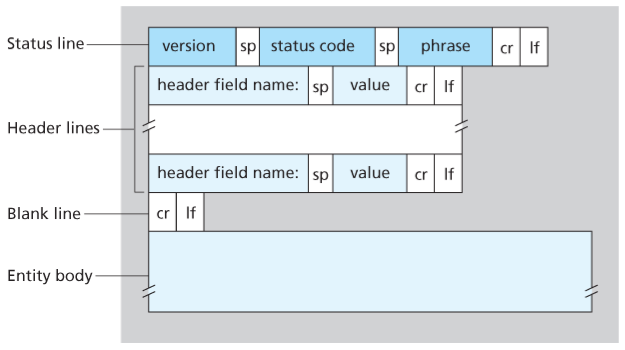
\includegraphics[width=\textwidth]{HTTPResponseMessage.png}
\caption{Forma generale di un messaggio di risposta HTTP}
\end{figure}
\subsection{Interazioni utente-server: Cookies}
HTTP \`e stateless in modo da permettere Web server con alte performance e in grado di gestire migliaia di connessioni TCP simultanee. Si rende per\`o desiderabile identificare utenti. Per questo motivo 
vengono utilizzati cookies che permettono di tenere traccia degli utenti. La tecnologia cookie ha quattro componenti: un header line nel messaggio HTTP di risposta, un header nel messaggio di richiesta HTTP, 
un file cookie tenuto sull'end system utente e gestito dal browser e un database back-end sul web site. Quando si compie un primo accesso ad un Web server si crea un numero unico di identificazione e crea 
un entry nel database indicizzato su quel numero. Il server poi risponde al browser includendo nella risposta HTTP \emph{Set-cookie:} che contiene il numero di identificazione. Quando il browser legge questa
linea appende una riga al cookie file che gestisce che include l'hostname e il numero di identificazione. Per gli accessi seguenti nell'header viene messo un cookie header che include il numero identificativo. 
\subsection{Web Caching}
Una Web cache o proxy server \`e un entit\`a della rete che soddisfa richieste HTTP al posto del web server originario. La cache possiede il proprio spazio di archiviazione che contiene copie di oggetti 
recentemente richiesti. Un browser pu\`o essere configurato in modo da tutte le richieste HTTP passino prima per la cache. Se questa non possiede il file inoltra la richiesta al server originario salvandola e 
poi inviandola all'utente. La cache \`e contemporaneamente un server e un client. Vengono utilizzate per aumentare la bandwidth e per ridurre il traffico verso i web server. Le web caches stanno prendendo un 
ruolo sempre pi\`u importante grazie a Content Distribution Networks (CDNs): una compagnia di CDN installa molte caches geograficamente distribuite localizzando il traffico. 
\subsubsection{Il GET condizionale}
Nonostante il caching possa ridurre il tempo di risposta percepito pu\`o introdurre il problema del controllo delle versioni dei file salvati in essa. Esiste un meccanismo in HTTP per permettere alla cache se i 
suoi file sono up-to-date: il \emph{GET} condizionale. Un get condizionale utilizza il metodo \emph{GET} e inserisce nell'header la linea \emph{If-modified-Since} il cui valore \`e nello stesso formato della
linea \emph{Last-modified}.
\section{Electronic mail}
E-mail \`e un mezzo di comunicazione asincrono veloce, facile da distribuire ed economico. Ogni utente possiede una mailbox locata in uno dei mail servers che mantiene e gestisce i messaggi che sono inviati
all'utente. Un messaggio tipico inizia nell'user agent del mittente e viaggia fino alla mail server del ricevente dove \`e depositata nella sua mailbox. Quando un utente vuole accedere ad un messaggio il mail 
server contenente la mailbox lo autentica. Se il server di spedizione non pu\`o inviare il messaggio nel server del ricevente il messaggio viene mantenuto un una message queue e prova a trasferire il messaggio 
pi\`u tardi. Ogni tentativo \`e fatto indicativamente ogni 30 minuti. Se non c'\`e successo dopo molti giorni il server rimuove il messaggio e notifica il mittente. SMTP \`e il protocollo application-layer principale. 
Utilizza TCP. SMTP ha due lati: lato client che viene eseguito sul mail server del mittente e un lato server eseguito sul mail server del ricevente. Entrambi i lati sono eseguiti su ogni mail server. 
\subsection{SMTP}
SMTP trasferisce i messaggi. Essendo molto precedente all'HTTP possiede certe caratteristiche arcaiche. Quando si invia un messaggio:
\begin{enumerate}
\item Il mittente invoca il suo user agent per e-mail, inserisce l'indirizzo e-mail del ricevente, compone un messaggio e dice all'user agent di inviarlo.
\item L'user agent del mittente invia il messaggio al suo mail server dove \`e posto in una message queue.
\item Dopo un SMTP handshaking iniziale il client SMTP invia il messaggio nella connessione TCP.
\item Al mail server del ricevente il lato server di SMTP riceve il messaggio e il mail server lo posiziona nella mail box del ricevente.
\item Il ricevente invoca il suo user agent per leggere il messaggio secondo la sua convenienza.
\end{enumerate}
SMTP solitamente non utilizza mail server intermedi. Per inviare i messaggi il client SMTP stabilisce una connessione alla porta 25 al server SMTP. Una volta che la connessione \`e stabilita si svolgono degli 
handshaking. Durante questa fase il client indica l'indirizzo e-mail del mittente e del ricevente. Dopo questa fase il client invia il messaggio. Il client successivamente ripete il processo sulla stessa connessione 
TCP se deve inviare altri messaggi altrimenti chiude la connessione. In un messaggio SMTP le righe con prefisso \emph{C:} sono le righe che il client invia nel socket TCP e quelle con prefisso \emph{S:} sono
quelle inviate dal server. Durante la comunicazione il client invia cinque comandi: \emph{HELO} seguito dal proprio mail server, \emph{MAIL FROM:} in cui \`e indicato l'indirizzo e-mail del mittente, 
\emph{RCPT TO:} dove \`e indicato l'indirizzo del ricevente \emph{DATA} contenenti il corpo dell'e-mail terminato da una singola riga contenente un punto e \emph{QUIT} per terminare la connessione. SMTP
utilizza connessioni persistenti. La prima riga contiene l'avvenuta connessione con il server del ricevente con il codice \emph{220}.
Per messaggi multimediali viene utilizzata l'estensione di SMTP MIME. 
\subsection{Comparazione con HTTP}
HTTP \`e primariamente un protocollo di pull, in particolare la connessione TCP \`e inizializzata dalla macchina che vuole ricevere il file. SMTP \`e primariamente un push protocol in quanto la connessione TCP 
\`e iniziata dalla macchina che vuole inviare i file. SMTP inoltre richiede che ogni parte del messaggio, compreso il corpo sia nello standard ASCII a 7 bit. Inoltre HTTP incapsula ogni oggetto in un diverso
messaggio HTTP, mentre in SMTP posiziona ogni oggetto del messaggio nel messaggio stesso.
\subsection{Formato dei messaggi mail}
Quando un messaggio e-mail \`e inviato informazioni secondarie sono contenute in una serie di righe header definite in RFC 5322 che ne specifica il formato esatto. Ogni riga header contiene testo leggibile che
consiste in parole chiave seguite dai due punti e un valore. Ogni header deve posseder un \emph{From:} e un \emph{To:}, pu\`o includere un \emph{Subject:}. Dopo l'header segue una riga vuota e il corpo del
messaggio. 
\subsection{Protocolli di accesso Mail}
Dopo che SMTP consegna il messaggio nel mail server e questo \`e posizionato nella mailbox del ricevente che lo visualizza attraverso un client. Solitamente le mailbox si trovano in mail server condivisi. Per 
accedere ai propri messaggi un protocollo speciale di accesso mail trasferisce i messaggi dal mail server all'end system del ricevente. Ne esistono vari tra cui Post Office Protocol-Version 3 (POP3), Internet
Mail Access Protocol (IMAP) e HTTP.
\subsubsection{POP3}
POP3 \`e definito nel RFC 1939 ed \`e semplice e con poche funzionalit\`a. POP3 comincia quando l'user agent apre una connessione TCP con il mail server sulla porta 110. Dopo averla aperta POP3 prosegue 
con l'autorizzazione, transazione e aggiornamento. Durante la prima fase l'user agent invia uno username  e una password in chiaro per autentificare l'utente. Durante la seconda fase l'user agent recupera i
messaggi e pu\`o marcarli per eliminazione e ottenere le statistiche della mail. La terza fase accade dopo il comando \emph{quit} che finisce la sessione POP3 e durante questa fase il mail server elimina i 
messaggi marcati per eliminazione. In una transazione POP3 l'user agent invia comandi e il server risponde con una risposta. Ce ne sono due possibili: \emph{+OK} seguita da dati server-to-client per indicare
il successo del comando e \emph{-ERR} usato dal server per indicare un errore con il comando. La fase di autorizzazione ha due comandi principali: \emph{user $<$username$>$} e \emph{
pass $<$password$>$}.  Durante la fase di transazione un user agente POP3 pu\`o essere configurato dall'utente per scaricare ed eliminare o scaricare e mantenere. La sequenza di comandi inviati dipende
da quale di questi due modelli viene utilizzato. Nel primo l'user agent invia il comando \emph{list, retr, dele}. POP3 \`e stateless.
\subsubsection{IMAP}
Con accesso POP3 il ricevente scarica i suoi messaggi sulla macchina locale, pu\`o creare cartelle mail e spostare mail scaricate in cartelle, cercare per messaggi. Questo paradigma pone un problema per 
un utente nomade che preferirebbe utilizzare una gerarchie di cartelle su un server remoto che pu\`o essere acceduto da ogni computer. Per risolvere questo problema nel RFC 3501 viene definito il protocollo 
IMAP. Possiede molte pi\`u capacit\`a del POP3 ma \`e anche significativamente pi\`u complesso. Un server IMAP associa ogni messaggio con una cartella e quando un messaggio arriva al server \`e associato 
con la cartella INBOX del ricevente che potr\`a poi spostarlo in una nuova cartella, leggerlo, eliminarlo, eccetera. Mette a disposizione comandi per permettere agli utenti di creare cartelle e spostare messaggi
da una all'altra e per cercare cartelle remote che corrispondono a criteri specifici. Un server IMAP mantiene informazioni sullo stato degli utenti. Inoltre possiede comandi che permettono agli user agent di
ottenere componenti dei messaggi. Per facilitare connessioni con bandwidth basso. 
\subsubsection{Web-Based E-Mail}
Con questo servizio l'user agent \`e un ordinario Web browser che comunica con la mailbox attraverso HTTP. 
\section{DNS - Internet's Directory Service}
Gli host dell'internet sono identificati da un hostname human readable e un indirizzo IP composto da quattro byte rappresentati
attraverso una dotted decimal notation che fornisce informazioni sulla posizione relativa dell'host nell'internet.
\subsection{Servizio di un DNS}
Per tradurre un hostname nel corrispondente indirizzo IP si crea un servizio di directory. Il ruolo principale del domain name system dell'internet \`e questo. Il DNS \`e un database distribuito implementato in
una gerarchia di server DNS e un protocollo di livello applicativo che  permette agli host di fare query su questo database. I server DNS sono macchine UNIX che eseguono il software Berkeley Internet Name 
Domain (BIND). Il protocollo DNS esegue UDP e usa la porta 53. \`E comunemente utilizzato da altri protocolli application layer come HTTP e SMTP per tradurre hostname in indirizzi IP:
\begin{enumerate}
\item La stessa macchina utente viene eseguita sul lato client di un'applicazione DNS.
\item Il browser estrae l'hostname dall'URL e lo passa al lato client dell'applicazione DNS.
\item Il lato client del DNS invia una query contenente l'hostname al server DNS.
\item Il client DNS riceve una risposta che contiene l'indirizzo IP corrispondente.
\item Una volta che il browser riceve l'indirizzo IP pu\`o iniziare una connessione TCP.
\end{enumerate}
Il DNS aggiunge un ritardo ulteriore alle applicazioni che lo utilizzano. Spesso gli indirizzi IP sono cachati in un DNS server locale in modo da ridurre il traffico verso i server DNS. Provvedono inoltre altri servizi:
\begin{itemize}
\item Host aliasing: un host con un nome complicato pu\`o avere uno o pi\`u alias. Il primo \`e detto hostname canonico.
\item Mail server aliasing. 
\item Load distribution: il DNS \`e utilizzato per distribuire il carico tra i server replicati. Quando siti sono replicati su diversi indirizzi IP il DNS invia tutta la lista ma ruota l'ordine degli indirizzi con ogni risposta. 
\`E utilizzato anche per i mail server.
\end{itemize}
Il DNS \`e specificato negli RFC 1034 e RFC 1035 e aggiornato in molti altri.
\subsection{Funzionamento del DNS}
Un design semplice per il DNS avrebbe un server DNS che contiene tutte le mappature da hostname a IP. \`E impraticabile in quanto:
\begin{itemize}
\item Possiede un singolo punto di fallimento.
\item Dovrebbe sostenere un volume di traffico immenso.
\item Il database centralizzato potrebbe essere troppo distante e pertanto introdurre un ritardo notevole.
\item Richiederebbe aggiornamenti troppo frequenti per ogni nuovo host.
\end{itemize}
Questo design fallisce in quanto non riesce a scalare. Per questo il DNS \`e distribuito.
\subsubsection{Un database distribuito e gerarchico}
Per gestire i problemi di scala il DNS utilizza un gran numero di server organizzati gerarchicamente e distribuiti geograficamente. Nessun server DNS contiene tutte le mappature. Ad una prima 
approssimazione esistono tre classi di DNS: server DNS radice, top-level domain (TLD) DNS e authoritative. Il client contatta la radice che ritorna l'IP di un TLD secondo l'ultimo dominio (.com) che a sua volta
ritorna un IP di un DNS authoritative. Oltre a questi esistono server DNS locali che non appartengono alla gerarchia ma si comportano da proxy per le richieste agli altri DNS. Una query DNS pu\`o essere 
iterativa (il DNS locale comunica solo con il DNS radice) o ricorsiva (il DNS locale comunica con tutti i DNS necessari). 
\subsubsection{DNS caching}
In una catena di query quando un DNS server riceve una risposta pu\`o cachare la mappatura nella sua memoria locale. Essendo host e mappature non permanenti le informazioni cachate sono scartate dopo un
periodo, tipicamente due giorni. 
\subsection{DNS records e messaggi}
I server DNS che implementano il database distribuito DNS salvano resource records (RRs) che includono quelli che forniscono la mappatura hostname-to-IP. Ogni messaggio di risposta DNS contiene
uno o pi\`u RRs. Un resource record \`e una tupla che contiene i campi \emph{(Name, Value, Type, TTL)}. \emph{TTL} \`e il tempo che rimane al RR e determina quando dovrebbe essere rimosso dalla cache. 
Il significato di \emph{Name} e \emph{Value} dipende da \emph{Type}:
\begin{itemize}
\item Se \emph{Type=A} allora \emph{Name} \`e un hostname e \emph{Value} \`e l'indirizzo IP. 
\item Se \emph{Type=NS} allora \emph{Name} \`e un dominio e \emph{Value} \`e l'hostname di un server authoritative DNS che sa come ottenere l'indirizzo IP.  \`E utilizzato per instradare query DNS lungo
la query chain.
\item Se \emph{Type=CNAME} allora \emph{Value} \`e l'hostname canonico per l'hostname halias \emph{Name}.
\item Se \emph{Type=MX} allora \emph{Value} \`e il nome del mail server canonico che ha un alias hostname \emph{Name}. 
\end{itemize}
Se un server DNS \`e authoritative per un particolare hostname contiene un record \emph{Type=A} per quell'hostname. Se non lo \`e contiene un record \emph{Type=NS} e uno \emph{Type=A} per il server 
DNS nel campo \emph{Value} del primo.
\subsubsection{Messaggi DNS}
Esistono due tipi di messaggio DNS: query e risposta e hanno lo stesso formato. 
\begin{itemize}
\item I primi 12 byte nella sezione header contengono vari campi:
\begin{itemize}
\item Il primo campo \`e un numero a 16 bit che identifica la query. \`E copiato nel messaggio di risposta in modo di verificare la corrispondenza tra query inviate e risposte ricevute.
\item Flags che indicano se il messaggio \`e una query o una risposta, una flag \`e settata in risposta se il DNS \`e authoritative, un altra se si desidera compiere della ricorsione, la cui disponibilit\`a \`e controllata
da un'altra. 
\item Quattro campi number-of che indicano il numero di occorrenze dei quattro tipi di sezioni dati che seguono l'header.
\end{itemize}
\item La question section contiene informazioni riguardanti la query che si sta svolgendo: include un campo di nome che contiene il nome che si sta richiedendo, un campo tipo che indica il tipo di domanda 
riguardo il nome.
\item In una risposta da un server DNS l'answer section contiene gli RRs per il nome che era stato originariamente richiesto che possono essere multipli.
\item L'authority section contiene records di altri servers authoritative.
\item L'additional section contiene altri record utili.
\end{itemize}
\subsubsection{Inserire records nel database DNS}
Esiste un registrar, un'entit\`a commerciale che verifica l'unicit\`a del nome di dominio, lo inserisce in un database DNS. Si devono fornire i nomi e indirizzi IP dei server DNS authoritative primari e secondari. Per ognuno di questi server authoritative il registrar fa in modo che record di tipo A e NS
siano registrati nei server TLD. E si deve fare attenzione ad inserire nel proprio server record di tipo A per il web server e di tipo MX per il mail 
server.
\section{Distribuzione di file Peer-to-Peer}
In un'architettura P2P esiste una minima o nessuna dipendenza verso un sistema centrale sempre attivo: intermittenetemente paia di hosts connessi detti peers 
comunicano direttamente tra di loro. Questi peers sono macchine controllate/possedute dagli utenti. Si consideri una naturale applicazione del P2P: la
distribuzione di file attraverso un protocollo detto bitTorrent in cui ogni peer pu\`o inviare una parte del file richiesto in modo da diminuire il carico
sul sistema centrale.
\subsection{Scalabilit\`a di architetture P2P}
Per considerare la naturale scalabilit\`a delle architetture P2P si consideri un modello di distribuzione file: si denoti il tasso di upload dell'access 
link del server con $u_s$, quello dell'i-esimo peer con $u_i$ e il tasso di download dell'i-esimo peer con $d_i$. Si indichi con $F$ la dimensione in bit
del file da distribuire e con $N$ il numero di peer a cui verr\`a distribuito tale file. Si intender\`a con tempo di distribuzione il tempo che verr\`a 
impiegato per distribuire il file a tutti i peers. 
\paragraph{Tempo di distribuzione client-server}
Si determini prima il tempo di distribuzione per le architetture client-server denotato con $D_{cs}$. Si 
osserva come il server deve distribuire completamente una copia ad ognuno degli $N$ peers e deve pertanto trasmettere $NF$ bits. Pertanto impiegher\`a 
$\frac{NF}{u_s}$ tempo. Sia ora $d_{\min}$ il tasso di download minimo tra i peers. Tale peer non potr\`a ricevere il file prima di $\frac{F}{d_{\min}}$. 
Attraverso queste osservazioni si nota come $D_{cs}=\max(\frac{NF}{u_s}, \frac{F}{d_{\min}})$. Si nota pertanto che il tempo di distribuzione cresce 
linearmente con il numero di peers $N$. 
\paragraph{Tempo di distribuzione P2P}
Calcolando il tempo di distribuzione per le architetture P2P si nota come un peer pu\`o assistere il server nell'invio dei dati utilizzando la propria 
capacit\`a di upload per inviarlo ad altri peers. Si consideri come all'inizio della distribuzione solo il server possiede il file. Per riuscire a inviare 
il file nella comunit\`a dei peers deve inviarlo almeno una volta attraverso il proprio access link, pertanto il tempo minimo \`e $\frac{F}{u_s}$. Il peer
con il tasso di download pi\`u basso non lo potr\`a ottenere prima di $\frac{F}{d_{\min}}$, rendendolo di fatto il tempo minimo. Si osservi come la 
capacit\`a di upload del sistema sia pari alla capacit\`a di upload del server e di tutti i peers, pertanto $u_{total}=u_s+u_0+\cdots u_N$. Tale sistema 
deve distribuire il file $F$ a tutti $N$ i peers, pertanto il tempo di distribuzione sar\`a $\frac{NF}{u_s+u_0+\cdots u_N}$. Unendo queste considerazioni si 
noti come il tempo di distribuzione diventa $D_{P2P}=\max\{\frac{F}{u_s}, \frac{F}{d_{\min}}, \frac{NF}{u_s+\sum\limits_{i=1}^Nu_i}\}$. Questo tempo non 
diventa pi\`u lineare con il numero di peers e pertanto provvede una scalabilit\`a implicita.
\subsection{BitTorrent}
BitTorrent \`e un popolare protocollo P2P in cui la collezione di peers che partecipano nella distribuzione di un file \`e chiamata torrent. I Peers in un
torrent scaricano chunks con stesse dimensioni (tipicamente 256 KBytes) del file l'uno con l'altro. Quando un peer si unisce ad un torrent all'inizio non
possiede nessun chunk, ma mentre comincia a scaricarli comincia anche a caricarli ad altri peers. Quando un peer acquisisce tutti i chunks potrebbe 
abbandonare il torrent o rimanerci in modo da continuare ad uploadare chunks ad altri utenti. Inoltre un peer potrebbe lasciare il torrent in qualsiasi 
momento per poi ritornarci quando desidera. Ogni torrent possiede un nodo infrastrutturale chiamato tracker. Quando un peer si unisce ad un torrent si 
registra con il tracker e lo informa periodicamente che si trova nel tracker. Quando questo avviene il tracker seleziona randomicamente un sottoinsieme di
peers tra i partecipanti a quello che si \`e appena aggiunto e invia a quest ultimo i loro IP. Attraverso questi IP il nuovo peer tenta di stabilire una
connessione TCP con ognuno di essi "peers vicini". Con il tempo questa lista cambia. Ad ogni istante ogni peer possiede un unico sottoinsieme di chunks. 
Periodicamente il peer richiede attraverso TCP ai suoi vicini la lista di chunk che possiedono e attraverso queste liste richiede i chunk che non possiede.
Pertanto ad ogni istante il peer sa quali chunk possiede e quali chunk possiedono i suoi vicini. Per decidere quali chunk richiedere si segue una politica
di "pi\`u rari prima" in modo da distribuire quelli meno presenti pi\`u velocemente ed equalizzando il numero di chunk nella rete. Per determinare a quali
richieste rispondere utilizza un algoritmo di trading. L'idea alla base \`e di dare priorit\`a ai richiedenti da cui sta ricevendo dati al tasso maggiore. 
Pi\`u specificatamente il peer monitora i tassi con cui riceve dati e determina i quattro peer che inviano il maggior numero di bit inviando loro i chunks.
Ogni 10 secondi questa lista viene aggiornata aggiornando i 4 peers "unchocked". Inoltre ogni 30 secondi sceglie un vicino randomicamente (optimistically 
unchocked). Questo permette che peers capaci di uploadare file a tassi compatibili comunichino tra di loro e a nuovi peers di ricevere dati. Tutti i peers
tranne questi 5 sono chocked, ovvero non ricevono nessun chunck dal peer. Questo meccanismo \`e conosciuto anche come tit-for-tat.
\section{Video streaming e content distribution networks}
Questi servizi sono implementati attraverso protocolli ad application-layer e servers che funzionano in maniera analoga a caches.
\subsection{Internet video}
In applicazioni di streaming di video salvati il video da distribuire \`e salvato in server e gli utenti inviano richieste al server per vedere i video on
demand. 
\subsubsection{Video}
Un video \`e una sequenza di immagini, tipicamente ad un frame fisso. Un video non compresso consiste in un array di pixels, ognuno dei quali codificato 
come un numero di bits che rappresentano colore e luminescenza. I video possono essere compressi, diminuendo la qualit\`a per ottenere un bit-rate pi\`u 
basso. Da un punto di vista di rete la caratteristica principale \`e il bit-rate che pu\`o essere di grande dimensione: pu\`o variare da $100\frac{kb}{s}$
fino a $10\frac{Mb}{s}$. Essendo la misura di performance per per streaming video \`e il throughput end-to-end. Per ottenere un playout continuo quest 
ultimo deve per lo meno eguagliare il bit-rate del video compresso. Si pu\`o utilizzare la compressione per creare diverse versioni dello stesso video in
modo da lasciar decidere all'utente in base alla propria bandwidth la versione da visualizzare. 
\subsection{HTTP streaming}
Nello streaming HTTP il video \`e salvato in un server HTTP come un file ordinario con un proprio URL. Quando l'utente vuole vedere il video stabilisce una
connessione TCP con il server e lancia una richiesta \emph{GET} per quell'URL. Il server successivamente invia il file pi\`u velocemente che pu\`o. Sul 
client side i bytes sono collezionati un un client application buffer. Quando il numero di bytes nel buffer superano un numero prestabilito l'applicazione
client inizia la riproduzione prendendo periodicamente da esso frame video, decomprimendoli e visualizzandoli. 
\subsection{DASH streaming}
Il protocollo DASH o dynamic adaptive streaming over HTTP nasce per premettere di codificare il video in molte versioni differenti ognuna delle quali con 
differente bit-rate e pertanto qualit\`a. Il client dinamicamente richiede chunks di video di pochi secondi selezionando la qualit\`a (e pertanto il bit-
rate) in base alla bandwidth disponibile in quel momento. I chunks sono richiesti attraverso singole richieste HTTP \emph{GET}. Con DASH ogni video \`e 
salvato nel server HTTP, ogni versione con un diverso URL. Il server HTTP possiede anche un manifest file che mette a disposizione gli URL per ogni versione
indicando il suo bit-rate. Il client richiede il manifest file in modo da conoscere le differenti versioni e richiede chunks da una di esse attraverso un
messaggio \emph{GET} specificando un URL e un byte range. Mentre scarica i chunks il client monitora la bandwidth di ricezione e lancia un algoritmo di rate 
determination per selezionare il chunk da richiedere successivamente. DASH permette pertanto di cambiare liberamente tra diverse qualit\`a. 
\subsection{Content distribution networks}
In modo da riuscire a distribuire enormi quantit\`a di dati a utenti distribuiti in tutto il mondo vengono utilizzate Content Distribution Networks (CDNs),
sistemi che gestiscono server distribuiti geograficamente salvando in ognuno di essi copie dei video e reindirizzando gli utenti verso i server che 
garantiscono la migliore esperienza. CDNs possono adottare una delle seguenti pratiche di server placement:
\begin{itemize}
\item Enter Deep: in questa pratica vengono creati server clusters in access ISPs in tutto il mondo in modo da essere vicini agli utenti finali, aumentando
il throughput diminuendo il numero di links tra server e client. La grande quantit\`a di server rende la gestione difficile. 
\item Bring home: in questa pratica portando a casa gli ISPs costruendo pochi server clusters vicino agli internet exchange points (IXPs), rendendo pi\`u 
semplice la loro gestione.
\end{itemize}
Una volta posizionati i cluster le CDNs replicano in essi i propri contenuti attraverso una push strategy: quando un video non presente sul cluster viene
richiesto tale richiesta viene girata ad un altro cluster che la invier\`a al cluster precedente e al client. Quando il cluster diventa pieno i 
video meno richiesti vengono eliminati. 
\subsubsection{CDN operation}
Quando un browser in host utente deve recuperare un video identificato da un URL il CDN deve intercettare la richiesta in modo da determinare un server
cluster adatto e reindirizzare la richiesta verso di esso. La maggior parte dei CDNs utilizzano il DNS per compiere questa azione. Quando un video viene
richiesto:
\begin{itemize}
\item L'utente visita la pagina web che lo contiene.
\item Quando l'utente seleziona il video viene inviata una query DNS con il dominio preceduto da \emph{video.}.
\item Il server DNS locale all'utente (LDNS) invia la richiesta verso un authoritative DNS che osserva la stringa \emph{video} e gira la query verso la CDN 
con l'indirizzo IP dell'utente che ritorna un hostname nel dominio del CNS all' LDNS.
\item Da questo punto la query entra nell'infrastruttura DNS privata del CDN: l'LDNS invia verso di esso una query DNS che ritorna un IP
\item L'LDNS invia all'utente l'indirizzo IP contenente il CND content server.
\item L'utente inizia una connessione TCP e lancia una richiesta HTTP \emph{GET}.
\end{itemize}
\subsubsection{Cluster selection strategies}
Alla base di un deployment CDN c\`e una cluster selection strategy, il meccanismo che reindirizza dinamicamente i client verso il content server 
appropriato. Dopo aver appreso l'IP del client il CDN deve decidere un cluster appropriato basandosi su di esso. Una strategia si basa sul selezionare
il cluster geograficamente pi\`u vicino. Oppure si possono monitorare i ritardi e le perdite di performance tra client e cluster attraverso periodici 
real-time measurment. Questi possono essere svolti attraverso ping ai LDNS.
\chapter{Transport Layer}
\section{Introduzione}
Il livello di trasporto ha il compito di mettere a disposizione la comunicazione direttamente tra i servizi applicativi eseguiti sui diversi host. Il 
livello di trasporto mette a disposizione comunicazione logica tra i processi applicativi, ovvero permette a questi processi di operare come se fossero 
direttamente connessi. I protocolli di livello di trasporto sono implementati negli end systems ma non nei routers di rete. Sul lato inviante il protocollo
trasforma il messaggio di livello applicativo in un pacchetto transport-layer conosciuto come segmento. Questo pu\`o essere fatto dividendo il messaggio in 
chunks pi\`u piccoli e aggiungendo ad ognuno di essi un transport-layer header. Il segmento \`e poi passato al network layer all'end system inviante dove
\`e incapsulato in un pacchetto network-layer (datagramma) e inviato alla destinazione. I router di rete non esaminano l'header del livello di trasporto.
Successivamente al ricevente il livello di rete estrae dal datagramma il segmento e il livello di trasporto lo processa rendendo i dati disponibili al
livello applicativo. 
\subsection{Relazione tra livello di trasporto e livelli di rete}
Se un protocollo di trasporto mette a disposizione comunicazione logica tra i processi i livelli di rete mettono a disposizione comunicazione logica tra i
diversi host. I protocolli di trasporto si trovano negli end systems e al loro interno muovono messaggi da processi applicativi al network edge e viceversa
ma non possono determinare come questi messaggi sono spostati nel network core. I servizi del livello di trasporto sono vincolati dalle politiche dei 
livelli di rete. Esistono comunque servizi che queste ultime non mettono a disposizione ma implementati unicamente dai protocolli di trasporto come 
affidabilit\`a e criptazione. 
\subsection{Livello di trasporto nell'internet}
L'internet mette a disposizione due protocolli per il livello di trasporto: UDP (user datagram protocol) che \`e un servizio connectionless e non affidabile 
alla persona che lo invoca e TCP (transmission control protocol) che \`e un servizio connection-oriented e affidabile. Quando progetta una applicazione di 
rete lo sviluppatore deve specificare uno di questi protocolli e fa questa scelta quando crea i socket. I pacchetti del livello di trasporto sono indicati
come segmenti anche se spesso si usa datagrammi per UDP e segmento per TCP. Si consideri un attimo il livello di rete dell'internet: IP questo protocollo
ha un modello di servizio best-effort delivery ma non fa garanzie sul successo della consegna ed \`e pertanto non affidabile. La responsabilit\`a 
fondamentale di UDP e TCP \`e estendere il servizio di consegna dell'IP da host a end systems, operazione chiamata transport-layer multiplexing e 
demultiplexing. Mettono a disposizione anche controlli di integrit\`a includendo campi per il controllo degli errori negli header. Questi due servizi sono
gli unici che UDP mette a disposizione. TCP invece mette a disposizione anche un data transfer affidabile utilizzando flow control, sequence numbers 
acknowledgements e timer garantisce che i dati siano trasferiti correttamente, completamente e in ordine. Oltre a questo TCP mette a disposizione un 
servizio di congestion control: un metodo per evitare che una connessione sia riempita e fatta rallentare con traffico eccessivo, provando a garantire ad 
ogni connessione lungo un link congestionato una parte uguale della bandwidth del link, regolando il tasso di upload dei bits nel sending side. Il traffico 
UDP non \`e regolato. 
\section{Multiplexing e demultiplexing}
All'host di destinazione il livello di trasporto riceve segmenti dal livello di rete e deve inviarli al livello applicativo del processo corretto. Si 
ricordi come ogni processo pu\`o avere pi\`u socket. Il livello di trasporto consegna i dati a questi socket, ognuno dei quali provvisto di un 
identificatore univoco. Il formato di questi identificatore dipende dal protocollo utilizzato. In modo che un host ricevente sia in grado di dirigere un 
segmento verso il socket appropriato possiede una serie di campi nell'header atti a questo scopo. Al lato ricevente l'host esamina questi campi per 
identificare il socket ricevente dove lo dirige. Questo processo \`e chiamato demultiplexing. Il processo di multiplexing consiste nel raccogliere chunks di 
dati dall'host sorgente da diversi socket, incapsularli con le informazioni header necessarie per creare i segmenti e poi passarli al livello di rete \`e 
chiamato multiplexing. Per permettere queste operazioni nell'header del livello di trasporto sono presenti due campi speciali che sono il campo del source 
port number e il destination port number. Ogni port number \`e un intero a 16 bit. I port number tra 0 e 1023 sono chiamati well-known port numbers e sono 
limitati in quanto utilizzati da protocolli conosciuti come HTTP. Quando si sviluppa una nuova applicazione si deve assegnare ad essa un port number. 
Risulta ora banale il demultiplexing: quando il livello di trasporto riceve un segmento legge questi campi e lo direziona verso il socket corretto. 
\subsection{Connectionless multiplexing e demultiplexing}
Quando un socket UDP \`e creato il livello di trasporto gli assegna una porta casuale che non sta venendo utilizzata da nessun altro socket. Si supponga che
in un Host A con porta UDP 19157 si vuole inviare un chunk di dati ad un processo UDP in Host B con porta 46428, il livello di trasporto in A crea un 
segmento che include i dati, la porta di source e la porta di destinazione e altri due valori. Il layer di trasporto lo passa poi al network layer che 
incapsula a sua volta il messaggio in un datagramma IP e tenta di consegnarlo al ricevente il cui transport layer legge la porta di destinazione a cui 
consegna il segmento al socket corrispondente. Host B pertanto compie il demultiplexing per consegnarlo al socket corretto. Si noti come un socket UDP \`e
completamente identificato da una tupla che consiste di un indirizzo IP di destinazione e o source port number. Pertanto se due segmenti hanno questi campi
uguali verranno entrambi rediretti verso lo stesso socket. Il source port number nel segmento serve a permettere una risposta ad A da parte di B. 
\subsection{Connection oriented multiplexing e demultiplexing}
Una socket \`e identificata da una tupla consistente di quattro valori: source IP address, source port number, destination IP address, destination port 
number, pertanto quando un segmento arriva ad un host utilizza questi quattro valori per reindirizzarlo verso la socket corretta. In particolare due 
segmenti TCP con diversi source IP addresses o source port number verranno indirizzati verso diversi sockets. L'applicazione server TCP possiede un 
welcoming socket che aspetta la richiesta di inizio di connessione dal client TCP il quale crea un socket e invia tale richiesta, costituita da un segmento
TCP costituito dal numero della porta di destinazione e un flag nell'header. Quando il server riceve tale richiesta crea un nuovo socket e salva port 
number, IP address di source e destinazione e mappa questi quattro valori con il socket su cui verranno reindirizzate attraverso il demultiplexing. 
\subsubsection{Web servers e TCP}
Si consideri un web server in un host sulla porta 80. Tutte le connessioni saranno stabilite su quella porta, successivamente una volta creato il socket
verranno reindirizzate su un socket univoco per ogni connessione.
\section{UDP}
UDP, definito nel RFC 768 \`e il protocollo di trasporto minimale, oltre a multiplexing e demultiplexing e minime funzioni di error checking non aggiunge 
niente all'IP. UDP prende i messaggi dall'applicazione, ci aggiunge i campi source e destination port numbers, un altro paio e passa il segmento 
al livello di rete che lo incapsula in un datagramma IP. Se il messaggio arriva a destinazione usa la destination port number per consegnarlo al socket. 
Un esempio di un protocollo applicativo che utilizza UDP \`e il DNS. I vantaggi rispetto al TCP sono:
\begin{itemize}
\item Maggiore controllo a livello di applicazione verso quali dati sono inviati e quando: con UDP appena un processo applicativo gli invia dati questi
vengono inviati, mentre il sistema di congestion control di TCP potrebbe rallentare questo processo. Viene pertanto utilizzato, con alcuni miglioramenti, 
per applicazioni a tempo reale.
\item Nessun connection establishment: e pertanto \`e pi\`u efficiente di TCP.
\item Nessun stato di connessione: non dovendo mantenere nessun stato riguardo la connessione un server che utilizza UDP pu\`o avere pi\`u utenti 
concorrenti.
\item Piccolo overhead per i pacchetti: il segmento UDP ha un header di soli 8 bytes. 
\end{itemize}
L'assenza del congestion control potrebbe comunque portare a grandi quantit\`a di perdita dati e il sovraffollamento di link. Data transfer affidabile pu\`o essere 
implementato anche con UDP se questo particolare viene implementato al livello applicativo. 
\subsection{Struttura dei segmenti UDP}
Il segmento UDP \`e composto da un campo dati che contiene il messaggio del livello applicativo. L'header possiede solo quattro campi, ognuno costituito da
due bytes: destination port number per il multiplexing, un campo per la lunghezza del segmento in bytes, il campo checksum per il controllo degli errori, il
source port number per la risposta.
\subsection{UDP checksum}
Il campo checksum \`e utilizzato per determinare se sono stati introdotti errori. UDP al livello di mittente svolge il complemento a uno della somma di 
tutte le 16-bit words nel segmento, con ogni overflow "wrapped around" e mette il risultato nel campo checksum. Il ricevente somma tutte le parole compreso 
il checksum e se non ci sono stati errori la somma deve ritornare $1111$ $1111$ $1111$ $1111$, se uno dei bit \`e zero sono stati introdotti degli errori. 
Nonostante UDP riesca a capire se c'\`e un errore non fa nulla per recuperarlo, alcune implementazioni eliminano i segmenti danneggiati, altre li mostrano
con uno warning. 
\section{Principi di data transfer affidabile}
\`E responsabilit\`a del reliable data transfer protocol di implementare l'astrazione di servizio che mette a disposizione canali attraverso i quali viene
messa a disposizione questo data transfer affidabile. In questo canale nessun bit \`e perso o corrotto e sono ricevuti nell'ordine di invio. Verranno 
considerati unicamente unidirectional data transfer.
\subsection{Costruire un protocollo di data transfer affidabile}
\subsubsection{Data transfer affidabile attraverso un canale perfettamente affidabile}
Quando il canale \`e perfettamente affidabile il protocollo accetta dati dal livello superiore, crea un pacchetto contenente i dati e invia il pacchetto nel
canale. Sul lato di ricezione il protocollo riceve un pacchetto dal livello sottostante, rimuove i dati dal pacchetto e li invia al livello soprastante. 
\subsubsection{Data transfer affidabile attraverso un canale con errori bit}
In questo caso nel canale possono essere corrotti dei bit. Questo tipo di errori accadono tipicamente nei componenti fisici. Per gestire questi errori 
si rende necessario un protocollo ARQ (automatic repeat request), che fa degli acknowledgments sia in caso di ricezione positiva che negativa. Oltre agli
acknowledgments il protocollo deve essere in grado:
\begin{itemize}
\item Error detection: bit esterni ai dati vengono aggiunti nel pacchetto e sono inviati dal mittente nel campo checksum per trovare se esistono degli 
errori.
\item Receiver feedback: l'unico modo per il mittente di conoscere lo stato del ricevente \`e se questo gli invia del feedback positivo (ACK) o negativo
(NAK), che in questo caso devono essere lunghi un solo bit. 
\item Retransmission: un pacchetto ricevuto con errore deve essere rinviato al destinatario. 
\end{itemize}
Quando il protocollo di invio deve inviare un messaggio aspetta che questo gli arrivi dai livelli superiori, quando lo riceve lo incapsula in un pacchetto
contenente anche il checksum e invia il pacchetto. A questo punto aspetta la ricezione di un ACK o un NAK. In caso del primo si rimette in attesa di un 
nuovo messaggio, altrimenti rinvia il messaggio precedente. Quando sta aspettando per l'acknowledgment non pu\`o ricevere altri messaggi dai livelli 
superiori, pertanto questo protocollo \`e conosciuto come stop-and-wait. Dal lato ricezione quando viene ricevuto un pacchetto si controlla per gli errori
e si invia l'acknowledgment appropriato. Se il mittente riceve un messaggio di acknowledgment corrotto rinvia il pacchetto e per questo errore viene 
introdotto il campo dei sequence number nel pacchetto, in modo da capire se il pacchetto \`e una ritrasmissione o no. Vengono pertanto utilizzati gli 
acknowledgments sia per il mittente che per il destinatario: quando un pacchetto out-of-order \`e ricevuto il destinatario invia un ACK per il pacchetto, 
quando riceve un pacchetto corrotto invia un NAK. Un mittente che riceve due ACK per lo stesso pacchetto sa che il destinatario non ha ricevuto 
correttamente il pacchetto seguente a quello ACKato due volte. 
\subsubsection{Data transfer affidabile attraverso un canale con errori bit che pu\`o perdere pacchetti}
Oltre a corrompere pacchetti questo canale pu\`o anche perderli. Si deve pertanto decidere cosa fare quando vengono persi dei pacchetti e cosa fare quando
questo succede. Quest ultimo problema \`e gestito dalle tecniche precedenti. Quando un pacchetto \`e perso il mittente non riceve nessuna risposta, 
pertanto deve aspettare fino a che \`e certo che il pacchetto sia stato perso e rinviarlo. I metodi visti precedentemente sanno gestire i pacchetti 
duplicati, pertanto i falsi positivi non sono un problema.
\subsection{Pipelined data transfer protocols}
Il problema con i protocolli precedenti \`e il fatto che sono stop and wait. Definita come utilization del mittente come la frazione di tempo in cui \`e 
impegnato ad inviare bit nella rete questo tipo di protocolli hanno 
\begin{equation*}
U_{sender}=\dfrac{packet\ size}{transmission\ rate\cdot round\ trip\ time}+
\dfrac{packet\ size}{transmission\ rate}
\end{equation*}
 che si nota essere una percentuale molto piccola del tempo di trasmissione totale. Per gestire questo problema
il mittente pu\`o inviare pacchetti multipli senza attendere una risposta con una tecnica conosciuta come pipelining che causa nel protocollo:
\begin{itemize}
\item Il range dei sequence number deve essere aumentato in quanto ogni pacchetto in transito deve avere un'identificatore unico. 
\item Mittente e destinatario devono poter fare del buffer su pi\`u pacchetti, quelli inviati ma su cui non \`e stato fatto acknowledgment e quelli ricevuti
correttamente dal destinatario.
\item Il range dei sequence number dipende su come il protocollo risponde a pacchetti persi o corrotti. 
\end{itemize}
\subsection{Go-Back-N (GBN)}
In un protocollo Go-Back-N il mittente pu\`o inviare numerosi pacchetti senza aspettare per l'acknowledgment ma non pu\`o avere pi\`u di un numero $N$ di 
pacchetti senza acknowledgement. Definita $base$ come il sequence number del pacchetto senza acknowledgment pi\`u vecchio e $nextseqnum$ il pi\`u piccolo
sequence number non utilizzato possono essere identificati quattro intervalli tra i sequence number:
\begin{itemize}
\item $[0, base-1]$ sono i pacchetti trasmessi e con acknowledgment.
\item $[base, nextseqnum-1]$ sono i pacchetti trasmessi ma senza acknowledgment.
\item $[nextseqnum, base+N-1]$ sono i sequence number che possono essere utilizzati per pacchetti che si possono spedire immediatamente.
\item $[base+N, \infty[$ sono i pacchetti che non possono essere utilizzati fino a che non ritorna l'acknowledgment di un pacchetto nella pipeline ($base$).
\end{itemize}
$N$ viene indicato come la window size di GBN che viene riferito come un protocollo sliding-window. Questo limite viene imposto per ragioni di congestion
control. Il mittente GBN deve poter rispondere a tre tipi di eventi:
\begin{itemize}
\item Invocation from above: quando il metodo di invio \`e chiamato dai livelli superiori il protocollo verifica che non ci siano $N$ pacchetti senza 
acknowledgment e se non succede crea e invia i pacchetto, altrimenti ritorna i dati al livello superiore o li mette in un buffer o ha un sistema 
sincronizzato di flag che permette la chiamata del metodo solo quando la window non \`e piena.
\item Receipt of an ACK: nel protocollo GBN un ACK per un pacchetto con sequence number $n$ viene considerato come un acknowledgment cumulativo, vale a dire
che tutti i pacchetti con sequence number minore uguale a $n$ sono stati ricevuti.
\item A timeout event: se accade un timeout il mittente rinvia tutti i pacchetti che sono stati inviati ma che non hanno ricevuto un acknowledgment.
\end{itemize}
Dalla parte del mittente quando questo riceve un pacchetto corretto ritorna un ACK con il sequence number, altrimenti lo elimina e invia un ACK per il
pacchetto precedente. In questo protocollo pacchetti non in ordine sono scartati in modo da semplificare il buffer del destinatario.
\subsection{Selective repeat}
Quando la window del GBN \`e larga pu\`o succedere che il protocollo sia costretto a ritrasmettere molti pacchetti. Il protocollo selective repeat evita
ritrasmissioni non necessarie facendo in modo che il mittente rinvii solo i pacchetti che sono stati persi o ricevuti corrotti dal mittente. Viene ancora
utilizzata una window $N$ per limitare il numero di pacchetti senza acknowledgment. Il destinatario quando riceve un pacchetto non in ordine fa 
acknowledgment e lo salva in un buffer fino a che non sono ricevuti tutti i pacchetti necessari. Si definisce pertanto $rcv\_base$ come il sequence number
del primo pacchetto mancante. Le azioni del mittente sono:
\begin{itemize}
\item Dati ricevuti dai livelli superiori: quando riceve dei dati il protocollo controlla per il prossimo sequence number, se la window lo permette crea il
pacchetto e lo invia, altrimenti \`e messo in un buffer o inviato al livello superiore come in GBN.
\item Timeout: timer sono utilizzati per decidere quando un pacchetto \`e andato perso e ogni pacchetto possiede il proprio timeout singolo. 
\item ACK ricevuto: quando \`e ricevuto il mittente marca il pacchetto come ricevuto e se il suo sequence number \`e uguale a $senderbase$ sposta la window
fino a che non trova un pacchetto senza acknowledgment e se ci sono pacchetti non trasmessi in essa vengono inviati.
\end{itemize}
Le azioni del destinatario sono:
\begin{itemize}
\item Pacchetto con sequence number in $[rcvbase, rcvbase+N-1]$ \`e ricevuto correttamente: viene inviato un selective ACK e se non era stato ricevuto 
precedentemente viene salvato nel buffer, se il suo sequence number \`e $rcvbase$ la window viene spostata inviando ricorsivamente tutti i pacchetti 
bufferati in sequenza.
\item Pacchetto con sequence number in $[rcvbase-N, rcvbase-1]$ \`e ricevuto correttamente: invia un ACK.
\item Se il pacchetto non si trova negli intervalli precedenti viene ignorato.
\end{itemize}
Il secondo punto \`e necessario per permettere alla window del mittente di muoversi in avanti. Si dimostra che la dimensione della window deve essere meno o 
uguale a met\`a della dimensione del sequence number space.
\section{Connection oriented transport: TCP}
TCP \`e definito in RFC 793, RFC 1122, RFC 1323, RFC 2018, and RFC 2581.
\subsection{La connessione TCP}
TCP \`e detto connection oriented perch\`e prima che un processo applicativo possa cominciare ad inviare dati deve compiere un handshake con il 
destinatario inviando dei segmenti preliminari per stabilire i parametri del data transfer. La connessione TCP \`e di tipo logico con lo stato comune 
che si trova unicamente sugli end-systems, pertanto gli elementi intermedi non mantengono uno stato TCP e le connessioni TCP gli sono completamente 
invisibili. Una connessione TCP mette a disposizione un servizio full-duplex: se esiste una connessione tra A e B i dati di livello applicativo possono
fluire sia da A a B che da B ad A contemporaneamente. Inoltre \`e sempre punto to punto, ovvero tra un singolo mittente e destinatario. Quando un client 
vuole iniziare una comunicazione con un server il processo applicativo del client informa il livello di trasporto che vuole iniziare una connessione con un
server su una particolare porta. Successivamente il TCP client inizia una connessione con il server TCP inviando un segmento TCP speciale a cui il server
risponde e alla fine il client risponde con un terzo segmento speciale. I primi due segmenti non trasportano payload, il terzo potrebbe. Questo procedimento
\`e chiamato three-way handshake. Una volta che la connessione TCP \`e stabilita i due host possono cominciare a scambiare dati. Il processo client invia 
uno stream di dati verso il socket che viene poi modificato dal TCP client che sposta i dati verso send buffer della connessione e periodicamente recupera
chunk di dati e li invia al livello di rete. Non sono fissati periodi specifici per questa azione e la dimensione massima dei chunk \`e definita come $MSS$
(maximum segment size) pari alla $MTU$ o maximum transmission unit. In modo che un segmento TCP e il corrispondente datagramma IP sia contenuto in un 
singolo frame di livello link. Un tipico valore di $MSS=1460Bytes$. TCP successivamente accoppia ogni chunk di dati con un header e lo passa al livello di 
rete dove \`e incapsulato con il datagramma IP che \`e poi inviato nella rete. Quando TCP riceve un segmento \`e piazzato nel receive buffer e 
l'applicazione legge lo stream dei dati da questo buffer. 
\subsection{Struttura dei segmenti TCP}
I segmenti TCP consistono un header e dati. I dati di livello applicativo, se troppo grandi sono divisi in chunk di dimensione $MSS$, cosa a volte non 
necessaria. L'header contiene: source e destination port numbers per il multiplexing, demultiplexing, un campo checksum e oltre a questi:
\begin{itemize}
\item Il campo sequence number di 32 bit e il 32 bit acknowledgement number field per implementare un data transfer affidabile.
\item La receive window di 16 bit per il flow control, per indicare il numero di byte che un destinatario \`e disposto a ricevere.
\item I campi delle opzioni opzionali e di lunghezza variabile utilizzati per negoziare $MSS$ o come un fattore di scalatura della window e un timestamp.
\item Il campo delle flag ha dimensione 6 bit e contiene: 
\begin{itemize}
\item Il bit ACK per indicare che il valore contenuto nel campo acknowledgement \`e valida, ovvero se il segmento 
contiene un acknowledgement per un segmento che \`e stato correttamente ricevuto.
\item I bit RST, SYN e FIN sono utilizzati per il setup e teardown della 
connessione.
\item CWR e ECE sono utilizzati in esplicite notifiche di congestion.
\item Il PSH che impone al ricevente di inviare i dati all'application layer
immediatamente.
\item Il bit URG che marca il segmento come contenente dati urgenti. 
\end{itemize}
\end{itemize}
\subsubsection{Sequence numbers e acknowledgement numbers}
Questi due campi sono chiave per il data transfer affidabile. Si consideri ora cosa TCP mette in questi campi: TCP considera i dati come uno stream di bytes 
non strutturato e non ordinato. L'uso dei sequence number riflette questa cosa in quanto questi numeri sono rispetto allo stream di bytes trasmessi e non
riguardo ai segmenti. Il sequence number di un segmento \`e il numero byte-stream del primo byte del payload. Il numero di acknowledgement per un ACK di un segmento \`e il sequence number del prossimo byte che ci si aspetta di ricevere. Nel TCP quando si riceve un acknowledgement per un byte vuol dire che tutti i byte precedenti sono stati ricevuti correttamente. Questo sistema si dice di acknowledgement cumulativi. Non \`e specificato cosa
fare in caso di segmenti non in ordine, ma viene implementata la scelta che non li scarta. Il numero iniziale della sequenza \`e scelto casualmente in modo
da minimizzare i casi di sequence number uguali per segmenti provenienti da diverse connessioni. 
\subsection{Stima del Round-trip time e timeout}
TCP utilizza un sistema di timeout/ritrasmissione per recuperare i pacchetti persi. Chiaramente questo timeout deve essere maggiore del round-trip time 
(RTT) come gestire i timeout TCP \`e stabilito nel RFC 6298.
\subsubsection{Stimare il round-trip time}
Si intende per $sampleRTT$ per un segmento come il tempo intercorso tra l'invio del segmento e la ricezione dell'acknowledgment. La maggior parte delle 
implementazioni TCP prendono un unica misura di RTT alla volta, ovvero ad ogni istante il $sampleRTT$ \`e stimato unicamente per uno dei pacchetti trasmessi
senza acknowledgment portando ad un nuovo valore di esso per ogni RTT e non computa tale valore per i pacchetti ritrasmessi. I valori di $sampleRTT$ 
varieranno per ogni segmento a causa della congestione dei router e dei payload sugli end-systems, pertanto per valutare un tipico RTT viene presa una media
tra tutti i $sampleRTT$. Pertanto TCP mantiene una media chiamata $estimatedRTT$ dei $sampleRTT$ calcolata come $$estimatedRTT=(1-\alpha)estimatedRTT+\alpha
sampleRTT$$, ovvero una combinazione pesata tra i due valori (con $\alpha=0.125$ consigliato). Si nota come questa combinazione mette particolare attenzione
verso i nuovi $sampleRTT$ in quanto riflettono meglio la situazione attuale. Questo tipo di media \`e chiamata exponential weighted moving average (EWMA) in
quanto il peso di un $sampleRTT$ decade esponenzialmente con l'aggiunta di nuovi valori. Oltre a questa stima \`e utile misurare la varianza di RTT, 
definita come $devRTT$, una misura di quanto un $estimateRTT$ varia rispetto a $estimatedRTT$ e calcolata come $$devRTT=(1-\beta)devRTT+\beta|sampleRTT-
estimatedRTT|$$, si noti come questo valore \`e una EWMA della differenza tra $estimatedRTT$ e $sampleRTT$, il valore raccomandato di $\beta$ \`e $0.25$.
\subsubsection{Settare e gestire il Timeout Retransmission Interval}
Il valore di un intervallo di timeout deve essere sicuramente maggiore di $estimatedRTT$, ma non cos\`i tanto da rendere la comunicazione inefficiente.
Si deve sommare pertanto a $estimatedRTT$ pi\`u un margine, la cui grandezza dipende dalle fluttuazioni di RTT, pertanto $TimeoutInterval=estimatedRTT+
4devRTT$. \`E raccomandato un valore iniziale di 1 e quando si trova un timeout il suo valore viene raddoppiato e quando un pacchetto \`e ricevuto 
l'intervallo viene ricomputato utilizzando la formula.
\subsection{Data transfer affidabile}
TCP crea un servizio di data transfer affidabile sopra un servizio inaffidabile del servizio IP di best-effort. Il servizio TCP garantisce che lo stream dei
dati che un processo legge dal buffer \`e non corrotto, senza buchi e duplicati e in sequenza. Il timer di ritrasmissione \`e unico per tutti i segmenti. Si 
supponga che i dati vengano inviati unicamente da A a B. In una prima discussione verranno utilizzati unicamente i timeout per recuperare i pacchetti persi.
Si nota che ci sono tre eventi che possono accadere nel sender: dati ricevuti dal livello applicativo, timer timeout e ACK. Quando TCP riceve dati dal
livello applicativo li incapsula in un segmento e li invia al livello di rete. Si nota come ogni segmento contenga un sequence number che \`e il byte-stream
number del primo byte contenuto e se il timer non \`e gi\`a stato avviato da qualche altro segmento TCP lo avvia quando il segmento \`e stato inviato al
livello inferiore. Il secondo evento \`e il timeout: in questo caso TCP ritrasmette il pacchetto e riavvia il timer. Il terzo evento \`e la ricezione di un 
ACK: lo compara con il valore $sendBase$ , ovvero il sequence number del pi\`u vecchio byte senza acknowledgment e utilizzando acknowledgment cumulativo
ne aggiorna il valore se il valore dell' ACK \`e del pacchetto successivo a quello di $sendBase$. 
\subsubsection{Raddoppiare l'intervallo di timeout}
Ogni volta che accade un timeout l'intervallo di timeout viene raddoppiato invece di calcolarlo come visto precedentemente in modo da mettere a disposizione
una forma limitata di congestion control. 
\subsubsection{Ritrasmissione veloce}
Un problema con la ritrasmissione governata da timeout \`e che quest ultimo pu\`o essere relativamente lungo aumentando il ritardo end-to-end, pertanto il 
mittente utilizza un altro sistema per determinare la perdita di pacchetti chiamato ACK duplicato. Un ACK duplicato \`e un pacchetto che rifa acknowledgment
su un pacchetto che ha gi\`a ricevuto un acknowledgment precedente. Si consideri pertanto la seguente tabella di politica di generazione degli ACK per
un destinatario:
\begin{center}
\begin{tabular}{|c|c|}
\hline
Event & Azione del destinatario TCP\\
\hline
\makecell{Arrivo in-ordine di un \\segmento tutti i dati fino a quel\\ sequence number sono stati\\ acknowledged} & \makecell{ACK ritardato: aspetta 
\\l'arrivo di un altro segmento \\ in ordine (500 msec),\\ se non succede invia un ACK}\\
\hline
\makecell{Arrivo in-ordine di un \\segmento con la presenza di un altro\\ segmento in order\\ senza acknowledgment} & \makecell{Invia un ACK cumulativo\\ACKing 
entrambi i segmenti}\\
\hline
\makecell{Arrivo di un segmento\\out-of-order, con sequence number\\maggiore, gap trovato} & \makecell{Invia un ACK duplicato\\indicando il sequence
\\number del prossimo byte aspettato}\\
\hline
\makecell{Arrivo di un segmento\\che riempie il gap} & \makecell{Se il sequence number\\ \`e all'inizio del gap \\ invia un ACK}\\
\hline
\end{tabular}
\end{center}
Si nota come quando un destinatario riceve un segmento out-of-order rifa acknowledgment dell'ultimo segmento in-order ricevuto. Se il mittente riceve tre
Quando si ricevono ACK duplicati per lo stesso segmento si considera il segmento immediatamente successivo come perso e viene compiuta una ritrasmissione prima
del timeout. Si nota come il meccanismo per la gestione degli errori \`e un misto tra i protocolli GBN e SR. 
\subsection{Flow control}
Si noti come ogni host TCP crea un buffer di ricezione per la connessione e quando la connessione TCP riceve dati che sono corretti e in ordine li posiziona
in tale buffer. L'applicazione associata legger\`a tali dati nel buffer, ma non necessariamente nell'istante in cui arrivano. Se questo non avviene pu\`o 
capitare che il buffer vada in overflow. TCP mette pertanto a disposizione un servizio di flow-control per eliminare questa possibilit\`a. Questo servizio
pertanto regola la velocit\`a rendendo uguale la velocit\`a con cui l'applicazione legge i dati con quella con cui i mittenti li invia. Per discutere di 
questo servizio si assuma che TCP scarti tutti i segmenti out-of-order. Il flow-control \`e messo a disposizione da TCP facendo in modo che il mittente
possieda una receive window, un modo che permette di capire al mittente quanto spazio nel buffer del ricevente \`e disponibile. Quando un host B deve
ricevere dati da un host A alloca un buffer e denota la sua dimensione con $rcvBuffer$, ogni tanto il livello applicativo in B legge i dati dal buffer. Si
definiscono pertanto le seguenti variabili $lastByRead$: il numero dell'ultimo byte letto dal processo applicativo nel buffer e $lastByteRcvd$: il numero 
dell'ultimo byte che \`e stato ricevuto e piazzato nel buffer. Essendo che TCP non permette overflow si deve avere: $lastByteRcvd-lastByteRead\le 
rcvBuffer$. Pertanto la receive window chiamata $rwnd$ \`e settata alla dimensione dello spazio rimanente nel buffer: $rwnd=rcvBuffer-(lastByteRcvd-
lastByteRead)$ e il valore di questa variabile cambia per tutta la durata della comunicazione. Per permettere il flow control B posiziona nel campo della
receive window $rwnd$ in ogni segmento che invia ad A. Inizialmente $rwnd=rcvBuffer$. Host A tiene in considerazione due variabili: $LastByteSent$ e 
$LastByteACKed$ la cui differenza \`e la quantit\`a di dati senza acknowledgment che A ha inviato nella connessione. Mantenendo questa differenza minore di
$rwnd$ si assicura l'assenza di overflow. Esiste un problema con questo schema: se il buffer \`e pieno e pertanto $rwnd=0$ e si supponga che dopo aver
avvisato che \`e pieno B non debba pi\`u mandare niente ad A, pertanto mentre B svuota il buffer non verr\`a notificato A che si \`e liberato dello spazio.
Per risolvere questo problema quanto $rwnd=0$ A continua a mandare segmenti con un data byte su cui sar\`a fatto acknowledgment da B, notificando pertanto A
quando si libera dello spazio. 
\subsection{TCP Connection Management}
Si consideri come una connessione TCP \`e inizializzata: si supponga di avere un processo client che vuole cominciare una comunicazione con un processo 
server. Il primo informa il client TCP che vuole iniziare una comunicazione con il secondo. Il client TCP inizializza la connessione con il server TCP in
questo modo:
\begin{itemize}
\item Il TCP client-side invia un segmento speciale al TCP server-side che non contiene nessun informazione del livello applicativo. Il flag dell'header TCP
SYN \`e settato a 1 (chiamato segmento SYN). Oltre a questo il client sceglie un sequence number randomico iniziale ($client_isn$) e lo mette nel campo 
sequence number del segmento SYN che \`e incapsulato in un datagramma IP e inviato al server. 
\item Una volta che il diagramma IP arriva al server questo ne estrae il segmento SYN, alloca il buffer TCP e i parametri di connessione e invia un segmento
di connection-granted al client che non contiene nessun dato di livello applicativo, il flag SYN settato a 1 e il campo acknowledgment settato a 
$client_isn+1$. Successivamente il server sceglie il proprio sequence number iniziale $server_isn$ e lo mette nel corrispettivo campo del segmento. Questo
segmento \`e chiamato segmento SYNACK.
\item Una volta ricevuto il segmento SYNACK il client alloca i buffer e i parametri di connessione e invia un segmento che fa acknowledgment al segmento 
SYNACK con il valore $server_isn+1$ nel campo acknowledgment e con flag SYN a 0. Quest'ultimo segmento potrebbe avere un payload. 
\end{itemize}
Una volta che questi tre segmenti sono stati inviati e ricevuti (three-way handshake) pu\`o iniziare la comunicazione tra client e server. Ognuna delle due
parti pu\`o terminare la connessione quando necessario. Quando quando questo succede buffer e variabili sono deallocate. Quando il client vuole terminare la
connessione invia un segmento speciale con il flag FIN settato a 1 a cui il server fa acknowledgment. Successivamente il server manda il proprio segmento di 
terminazione (con FIN settato) e il client fa acknowledgment. A questo punto entrambi deallocano le risorse. Durante la vita di una connessione TCP il protocollo in ogni host
fa delle transizioni tra stati TCP: il client TCP inizia nello stato CLOSED, poi l'applicazione inizia una connessione che causa l'invio del segmento SYN e 
a TCP di entrare nello stato SYN\_SENT dove aspetta per l'acknowledgment che lo fa entrare nello stato ESTABLISHED. Quando il client vuole terminare la 
comunicazione invia il segmento con il bit FIN a 1 ed entra nello stato FIN\_WAIT\_1 dove aspetta l'acknowledgment; quando lo riceve entra nello stato 
FIN\_WAIT\_2 dove aspetta il segmento di chiusura del server che causa la transizione nello stato TIME\_WAIT che permette di rinviare l'ACK finale se \`e 
stato perso (dai 30 secondi ai 2 minuti), successivamente entra nello stato CLOSED. Il server
pu\`o decidere di chiudere la comunicazione in modo "rude": dealloca le risorse e chiude la porta. Quando il client tenta di comunicare su quella porta il pacchetto viene bloccato dal
server e viene ritornato un segmento con il flag RST settato.
\section{Principi di congestion control}
Per gestire la congestione della rete si devono rallentare i mittenti che operano in tale rete. 
\subsection{Cause e costi della congestione}
Si considerino ora tre casi in cui pu\`o avvenire della congestione. 
\subsubsection{Due mittenti, router con buffer infiniti}
Si consideri uno scenario in cui ci sono due mittenti A e B che comunicano attraverso un unico router. Si assuma che A invii dati nella connessione ad un 
tasso medio di $\lambda_{in}\frac{bytes}{sec}$ che \`e pertanto il tasso con cui A passa dati al router. B opera in maniera simile e si presuppone che anche
lui invii dati con un tasso medio di $\lambda_{in}\frac{bytes}{sec}$. I pacchetti da A e B passano attraverso un router e sopra un link condiviso di 
capacit\`a R. Il router possiede infiniti buffer che gli permettono di memorizzare i pacchetti che gli arrivano quando il tasso di arrivo supera R. 
Analizzando il per-connection throughput (numero di bytes al secondo che arrivano al destinatario), per un tasso di invio tra 0 e $\frac{R}{2}$ tale 
throughput \`e uguale al tasso di invio e il delay rimane un numero finito.  Quando il tasso di invio supera $\frac{R}{2}$ tale throughput rimane $\frac{R}
{2}$, ma il delay diventa infinito in quanto il numero di pacchetti in coda al router aumenta in maniera incontrollata. Si noti pertanto come se i pacchetti 
arrivano a velocit\`a simile alla capacit\`a del link si ha esperienza di grandi ritardi causati dalle code sui router. 
\subsubsection{Due mittenti, router con buffer finiti}
Si modifichi lo scenario precedente considerando buffer finiti: si assuma una connessione affidabile e un pacchetto che entra in un buffer pieno viene
perso. Se un pacchetto viene perso verr\`a eventualmente ritrasmesso. Si differenzi pertanto tra il tasso di trasmissione di dati originali come $
\lambda_{in}\frac{bytes}{sec}$ e quello totale come $\lambda'_{in}\frac{byytes}{sec}$ chiamato come offered load alla rete. Le prestazioni definite nello 
scenario precedente dipenderanno ora fortemente da come avviene la ritrasmissione. Se A fosse capace di stabilire quando un buffer \`e pieno $
\lambda_{in}=\lambda'_{in}$ e il throughput della connessione sarebbe $\lambda_{in}$ in questo caso il tasso di invio non pu\`o superare $\frac{R}{2}$. Si 
consideri il caso in cui il mittente rinvia il pacchetto \`e dato certamente per perso, si consideri un'offered load $\lambda'_{in}=\frac{R}{2}$, a questo 
valore il tasso di ricezione di dati reali per il destinatario \`e $\frac{R}{3}$, pertanto sui $0.5R$ dei dati trasmessi $0.1\bar{6}R$ sono ritrasmessi. Si 
nota pertanto ulteriore costi di una rete congestionata: la ritrasmissione di pacchetti persi dovuta al buffer overflow e il rinvio di pacchetti in coda nel
router dati per persi che pertanto vengono rinviati fino al destinatario che li scarta (se succede per ogni pacchetto il throughput avr\`a un valore
asintotico di $\frac{R}{4}$).
\subsubsection{Quattro mittenti, router con buffer finiti e cammini multihop}
In questo scenario quattro host trasmettono dati ognuno attraverso sovrapposti cammini a due hops. Si assume che ogni host utilizza un meccanismo di 
timeout/ritrasmissione per implementare un data transfer affidabile, che hanno tutti lo stesso valore $\lambda_{in}$ e tutti i router hanno capacit\`a
$R\frac{bytes}{sec}$. Si consideri la connessione tra A e C che passa tra i router $R_1$ e $R_2$ e che condivide  $R_1$ con la connessione D-B. Per valori
bassi di $\lambda_{in}$ i buffer overflow sono rari e pertanto aumenti in $\lambda_{in}$ sono pari ad aumenti di $\lambda_{out}$. Si consideri ora il caso
in cui $\lambda_{in}$ e pertanto $\lambda'_{in}$ sono estremamente grandi e si consideri $R_2$: il traffico A-C che arriva a $R_2$ (forwarded da $R_1$) 
pu\`o avere al massimo R, la capacit\`a del link da $R_1$ a $R_2$. Se $\lambda'_{in}$ \`e estremamente grande anche per la connessione B-D. Essendo che 
le connessioni A-C e B-D devono competere a $R_1$ per la capacit\`a dei buffer il traffico A-C che arriva a $R_2$ diventa minore con l'aumentare di 
$\lambda'_{in}$. Nel caso limite un buffer vuoto a $R_2$ viene completamente riempito da pacchetti B-D e pertanto il tasso di connessione end-to-end 
di A-C diventa 0. Pertanto si aggiunge un ulteriore costo alla perdita di un pacchetto a causa della congestione: quando un pacchetto \`e perso lungo un 
cammino la capacit\`a di trasmissione utilizzata nei link upstream fino al punto dove \`e perso viene sprecata. 
\subsection{Approcci al congestion control}
Si distinguono due approcci al congestion control in base al fatto che il livello di rete aiuta a gestire il problema della congestion o no.
\begin{itemize}
\item End-to-end congestion control: il livello di rete non mette a disposizione nessun aiuto. Anche la presenza di congestione deve essere inferita 
osservando il comportamento della rete. \`E quello utilizzato dal TCP che utilizza la perdita di pacchetti come segnale, riducendo la dimensione della 
window. Oltre alla perdita di pacchetti possono venire considerati gli aumenti del round-trip segment delay. 
\item Network-assisted congestion control: il router mette a disposizione feedback esplicito sulla condizione della rete o con un bit che notifica la 
presenza di congestione o con la capacit\`a massima di ricezione dell'altra parte della comunicazione. Questa informazione \`e ricevuta direttamente dal 
router con un chocked segmento o dal destinatario in cui il router marca il segmento. 
\end{itemize}
\section{TCP congestion control}
TCP utilizza un meccanismo di congestion control end-to-end. TCP limita il tasso a cui ogni mittente invia pacchetti nella rete attraverso una funzione
di percepita congestione.
\subsubsection{Limitare il tasso del mittente}
Si ricordi come ogni connessione TCP consiste di un buffer di ricezione, uno di invio e multiple variabili. Il meccanismo di congestion control del TCP del
mittente opera su un'ulteriore variabile chiamata congestion window $cwnd$ che impone una limitazione al tasso di invio di dati nella rete facendo in modo
che la quantit\`a di dati senza acknowledgment sia inferiore al minimo tra $cwnd$ e $rwnd$: $LastByteSent-LastByteACKed\le\min(cwnd, rwnd)$. Si assuma ora
che il buffer di ricezione sia cos\`i grande che $rwnd$ possa essere ignorata: il tasso di invio sar\`a $\frac{cwnd}{RTT}\frac{bytes}{sec}$. Variando il
valore di $cwnd$ si cambia il tasso di trasmissione. 
\subsubsection{Percepire congestione}
Si definisca un evento di perdita l'occorrenza di un timeout o di tre ACK sullo stesso pacchetto consecutivi. Quando c'\`e congestione eccessiva uno o pi\`u
router sul cammino comincer\`a a perdere segmenti causando l'evento di perdita che viene considerato come un segnale di congestione del cammino. In assenza
di perdite la congestion window viene aumentata tanto velocemente quanto arrivano gli acknowledgment. Per questo motivo TCP viene chiamato self-clocking. 
\begin{itemize}
\item Un segmento perso implica congestione e pertanto il tasso del mittente TCP deve essere diminuito.
\item Un segmento di acknowledgment implica che la rete sta consegnando i pacchetti e pertanto il tasso del mittente pu\`o essere aumentato quando arriva
un ACK per un segmento senza acknowledgment.
\item Bandwidth probing: aumentando mano a mano il tasso di trasmissione TCP tenta di arrivare al limite per cui la rete comincia a congestionarsi, 
arrivando cos\`i al massimo valore sopportabile da essa.
\end{itemize}
Si pu\`o pertanto descrivere l'algoritmo di congestion control del TCP composto da slow start, congestion avoidance e fast recovery i primi due sono 
obbligatori e differiscono per come variano il valore di $cwnd$ mentre il terzo \`e facoltativo.
\subsubsection{Slow start}
Quando una connessione TCP comincia il valore di $cwnd$ \`e inizialmente settato a $1\ MSS$. Essendo la quantit\`a di bandwidth spesso molto pi\`u grande
tale valore aumenta velocemente di $1\ MSS$ per ogni segmento di acknowledgment ricevuto in modo che il tasso di invio aumenti esponenzialmente. Quando si
verifica un evento di perdita causato da un timeout il mittente setta il valore di $cwnd$ a $1\ MSS$ e ricomincia il processo di nuovo settando una nuova 
variabile chiamata $sstresh$ a $\frac{cwnd}{2}$. Successivamente $cwnd$ viene di nuovo fatto aumentare fino a che raggiunge o supera il valore di $sstresh$,
dove slow start termina e TCP si sposta in congestion avoidance. Se tre ACKs duplicati sono ricevuti TCP svolge un fast retrasmit e entra nello stato di 
fast recovery. 
\subsubsection{Congestion avoidance}
Quando si arriva nella modalit\`a di congestion avoidance $cwnd$ \`e pi\`u o meno la met\`a del valore in cui era iniziata la congestione. Si deve pertanto
aumentare il suo valore con pi\`u cautela, pertanto aumenta il suo valore di $1\ MSS$ ogni RTT. Questo \`e fatto aumentando $cwns$ di un valore $\frac{MSS}
{cwnd}$ ogni volta che un nuovo acknowledgment arriva. Quando accade un timeout si aggiorna il valore di $sstresh$, $cwnd$ viene impostato a $1\ MSS$ e si
ritorna in slow start mode. Se si ricevono tre ACK consecutivi dimezza il valore di $sstresh$  e si pone $cwnd=sstresh+3\ MSS$ e entra nello stato di fast recovery.
\subsubsection{Fast recovery}
Il valore di $cwnd$ \`e aumentato di $1\ MSS$ per ogni ACK duplicato del segmento mancante che ha causato TCP di entrare in questo stato. Quando un ACK 
arriva per il segmento mancante entra nello stato di congestion avoidance dopo aver diminuito il valore di $cwnd$. Se succede un timeout performa le stesse
azioni degli altri due stati.
\subsection{Fairness}
Si considerino $k$ connessioni TCP con cammini diversi ma tutte passanti attraverso un link di bottleneck con un tasso di trasmissione $R$. Supponendo
che ogni connessione invii una grande quantit\`a di dati un meccanismo di congestion control \`e detto fair se ognuno dei tassi di trasmissione per le 
connessioni \`e $\frac{R}{k}$. Si consideri il caso in cui $k=2$. Entrambe con lo stesso $MSS$ e $RTT$. Si ignori la fase di slow start e si assuma che 
entrambe le connessioni siano nello stato di CA, ovvero AIMD (additive increase multiplicative decrease). Si noti che attraverso questo meccanismo entrambe
le connessioni fluttueranno intorno al valore di tasso di trasmissione pari a $\frac{R}{2}$. Considerando una situazione reale le connessioni con RTT basso
sono pi\`u veloci a capire un'assenza di connessione e avranno pertanto una maggiore porzione della banda. A differenza del TCP UDP non \`e fair. Il 
meccanismo pu\`o essere sfruttato per ottenere pi\`u banda aprendo pi\`u connessioni TCP parallele.
\subsection{Explicit congestion notification, network-assisted congestion control}
Estensioni di TCP e IP sono state implementate per permettere al livello di rete di notificare la presenza di congestione attraverso l'explicit congestion
notification. Al livello di rete due bit nel campo di Type of Service del header del datagramma IP sono utilizzate per l'ECN. Uno dei settings di questi 
bit sono modificati dal router per notificare la congestione. Questa indicazione viene poi riportata dal datagramma al destinatario. Un secondo bit \`e 
utilizzato per indicare che il router \`e ECN-capable. Quando il destinatario riceve il datagramma marcato informa il TCP nel mittente settando l'ECE 
(explicit congestion notification echo) bit nel segmento di ACK. Il mittente reagisce a questo ACK come ad un evento di perdita e setta il bit di CWR
(congestion window reduced).

\chapter{Il livello di rete: data plane}
\section{Considerazioni sul livello di rete}
A differenza dei livelli precedenti il livello di rete si trova anche nei router e negli elementi nel network core. Il ruolo primario del data plane nel 
livello di rete di ogni router\`e quello di permettere il forwarding dei datagrammi dai suoi input links verso gli output links, il ruolo primario del 
control plane \`e di coordinare queste operazioni di forwarding per router in modo che il datagramma arrivi a destinazione. 
\subsection{Forwarding e routing: il data e control plane}
Il roulo primario del livello di rete \`e quello di muovere dati dal mittente al destinatario. Affinch\`e questo avvenga vegono individuate due funzioni
fondamentali:
\begin{itemize}
\item Forwarding: quando un pacchetto arriva ad un router input link deve essere spostato nell'appropriato output link. Tale pacchetto pu\`o essere anche 
bloccato o copiato e mandato a multipli destinatari.
\item Routing: il livello di rete deve saper determinare la route o il cammino preso dal pacchetto mentre si sposta dal mittente al destinatario. 
L'algoritmo che implementa questa funzionalit\`a \`e detto algoritmo di routing.
\end{itemize}
Un elemento chiave in ogni router \`e la sua tabella di forwarding: un router forwards un pacchetto controllando i valori di alcuni campi nell'header e 
usando questi valori per indicizzare la tabella. Il valore salvato per quei campi indica il link di output dove deve essere mandato il pacchetto. 
\subsubsection{Approccio tradizionale al control plane}
Le tabelle di forwarding sono determinate da un algoritmo di routing che viene eseguito su ogni router e pertanto entrambe le funzioni di forwarding e di
routing sono contenute in esso. La funzione dell'algoritmo di routing di un router comunica con altre attraverso per computare i valori della tabella di 
forwarding. Questa comunicazione avviene attraverso un protocollo di routing. 
\subsubsection{Approccio SDN al control plane}
In questo approccio le tabelle di routing sono computate e distribuite da un controller separato fisicamente dai router e il router possiede solo la 
funzione di forwarding. La comunicazione tra questi elementi avviene attraverso lo scambio di messaggi contenenti le tabelle di routing e altre componenti. 
Questo approccio \`e al centro del software-defined networking (SDN) in quanto il controller \`e implementato in software. 
\subsection{Network service model}
Il network service model determina le caratteristiche dei servizi offerti dal livello di rete. Possono essere:
\begin{multicols}{2}
\begin{itemize}
\item Consegna garantita.
\item Consegna garantita con ritardo limitato.
\item Consegna di pacchetti in ordine.
\item Sicurezza.
\end{itemize}
\end{multicols}
Il livello di rete garantisce un solo servizio: il servizio di best-effort. In questo servizio n\`e la consegna n\`e l'ordine sono garantiti.
\section{Componenti di un router}
\begin{figure}[h]
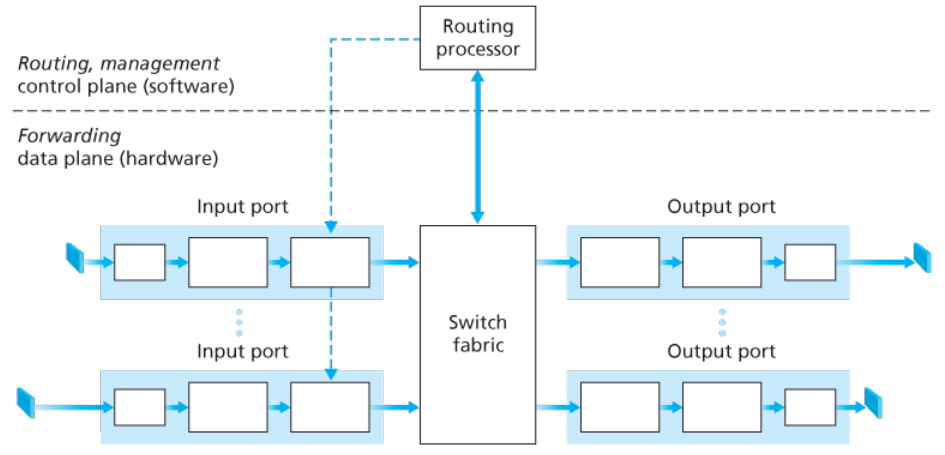
\includegraphics[width=\textwidth]{Router.png}
\caption{Architettura di un router}
\end{figure}
\begin{itemize}
\item Porte di input: una porta di input svolge la funzione di livello fisico di interrompere un link fisico entrante nel router, funzioni di livello di 
link necessarie per interoperare con il livello di link all'altro capo del link. Inoltre viene anche svolta una funzione di lookup dove viene consultata la 
tabella di forwarding per determinare a quale porta di output verr\`a forwarded il pacchetto attraverso la switching fabric. I pacchetti di controllo sono
forwarded da una porta di input al processore del router.
\item Switching fabric: questa componente connette le porte di input con le porte di output e costituisce essa stessa una rete. 
\item Porte di output: questa componenente salva i pacchetti ricevuti dalla switching fabric e li trasmette al link facendo le necessarie operazioni 
di livello di link e fisico. Quando il link \`e bidirezionale la porta corrispondente di input viene accoppiata a quella di output. 
\item Processore di routing: svolge funzioni di control plane: nei router tradizionali esegue il protocollo di routing , mantiene le tabelle di routing e 
relative informazioni di link state e computa la tabella di forwarding. Nei router SDN \`e responsabile per la comunicazione con il controller. Svolge oltre
funzioni di gestione della rete.
\end{itemize}
A causa della necessit\`a di operare a velocit\`a elevatissime tutte queste componenti sono implementate in hardware.
\subsection{Processi alle porte di input e forwarding basato sulla destinazione}
Le funzioni di line termination e di livello di link processing della porta di input implementano il livello di link e fisico per quel link di input. Il 
lookup svolto nella porta di input \`e centrale per le funzioni del router: qui viene utilizzata la tabella di forwarding per detrminare la porta di input
al quale il pacchetto dovr\`a essere inviato attraverso la switching fabric. La tabella di forwarding \`e computata dal processore di routing o ricevuta dal
controller. La tabella di routing \`e copiata dal processore alla porta di input attraverso un bus diverso in modo da evitare un bottleneck causato dalla
chiamata di un processo centrale. Si consideri ora il caso in cui la porta di output \`e determinata unicamente dall'indirizzo di destinazione: a causa
del gran numero di indirizzi possibili non \`e possibile utilizzare un algoritmo brute-force. Per migliorare le prestazioni si utilizza una regola di 
longest prefix matching: il router ritorna dalla tabella l'indirizzo tale per cui attraverso il lookup si \`e trovato il pi\`u lungo prefisso 
corrispondente. Vengono inoltre utilizzate tecniche pi\`u efficienti di una ricerca lineare come la memorizzazione delle tabelle in DRAM con SRAM come
cache o ternary content addressable memory (TCAM). Una volta che la destinazione del pacchetto \`e stata determinata entra nella switching fabric. In alcuni
casi un pacchetto potrebbe essere temporaneamente bloccato se pacchetti da altre porte la stanno utilizzando, venendo posto in una coda e programmato per
entrare nella switching fabric in un secondo momento. Oltre al lookup devono comunque essere svolte altre operazioni: processamento al livello fisico e di
link, i campi di numero di versione, checksum e time-to-live devono essere controllati e gli ultimi due riscritti e i contatori per la gestione di rete 
devono essere aggiornati.
\subsection{Switching}
Lo switching pu\`o essere ottenuto in vari modi:
\begin{itemize}
\item Switching attraverso la memoria: nei primi router, normali computer una porta di input notificava il processore di routing attraverso un interrupt 
dell'arrivo di un pacchetto che veniva copiato dalla porta nella memoria del processore che estraeva l'header, svolgeva l'operazione di lookup e lo copiava
nel buffer della porta di output. 
\item Switching attraverso un bus: in questo approccio la porta di input trasferisce il pacchetto direttamente verso la porta di output lungo un bus 
condiviso. Tutte le porte di output ricevono il pacchetto ma solo quella appropriata lo mantiene. Solo un pacchetto alla volta pu\`o trovarsi nel bus.
\item Switching attravreso una rete di interconnessione: si utilizza un crossbar switch che consiste di $2N$ bus che connettono $N$ porte di input ad 
altrettante porte di output. Ogni bus verticale si interseca con uno orizzontale ad un crosspoint che pu\`o essere aperto o chiuso. Un pacchetto da A a Y
trover\`a chiuso il crosspoint nell'intersezione dei bus di A e Y. Questo switch si dice non bloccante in quanto un pacchetto pu\`o attraversarlo a patto 
che non abbia lo stesso output di un altro.
\end{itemize}
\subsection{Processing delle porte di output}
Le porte di output prendono i pacchetti nei corrispettivi buffer, li selezionano, li rimuovono dal buffer, svolgono le funzioni di livello di link e fisico
e inviano il pacchetto al link.
\subsection{Queuing}
Le code di pacchetti possono accadere nei buffer delle porte di input o in quelli delle porte di output. La dimensione di queste code dipende dalla 
quantit\`a di traffico, dalla velocit\`a della switching fabric e dalla velocit\`a della linea. \`E quando queste code vengono riempite fino al massimo che
vengono persi dei pacchetti. Si supponga che le linee di input e output abbiano tutte la stessa velocit\`a $R_{line}$ e che ce ne sono $N$ per tipo. Si 
assuma che tutti i pacchetti abbiano una lunghezza fissa e arrivino alle porte in maniera sincrona. Si definisca $R_{switch}$ il tasso di trasmissione della
switching fabric. Se questo \`e uguale a $NR_{line}$ nessuna coda verr\`a creata alle porte di input. 
\subsubsection{Input queuing}
In caso che $R_{switch}$ sia minore di $NR_{line}$ pu\`o succedere che pacchetti debbano essere messi in coda nell'attesa che vengano inviati alle porte di
input. Si supponga una crossbar switching fabric con velocit\`a di link identiche e che un pacchetto possa essere trasferito ad una porta di output nello
stesso tempo in cui viene ricevuto dal link di input e i pacchetti sono mossi verso l'output in modo FCFS (first-come first-served), pacchetti multipli 
possono essere trasferiti simultaneamente a patto che abbiano output diversi. Pu\`o nascere un evento di head-of-the-line blocking (HOL) in quanto un 
pacchetto incodato deve aspettare per il trasferimento perch\`e quello prima di lui \`e bloccato da un altro. A causa di questo evento la coda potrebbe 
crescere illimitatamente e pertanto causare perdita di dati.
\subsubsection{Output queuing}
Si supponga $R_{switch}$ uguale  $NR_{line}$ e che gli $N$ pacchetti che arrivano da ognuna delle porte di input debbano essere inviati nella stessa porta 
di output. In questo caso durante la trasmissione di un pacchetto arrivano alla porta $N$ nuovi pacchetti e questi dovranno essere incodati. Eventualmente
questa coda si potrebbe riempire causando perdita di pacchetti. Quando non c'\`e pi\`u abbastanza memoria per salvare un pacchetto si deve scegliere se 
droppare il pacchetto appena arrivato (drop-tail) o uno in coda. Un'altra azione potrebbe essere quella di marcare un pacchetto prima che questo si 
verifichi in modo da inforamare dell'esistenza di congestione. Un numero di regole di packet dropping e marking \`e conosciuto come active queue management
(AQM). Uno dei pi\`u diffusi \`e il random early detection (RED). Una conseguenza di questo incodamento \`e che un packet scheduler alla porta di output 
deve decidere quale pacchetto trasmettere. Le dimensioni della coda variano e vengono scelte in base  a $RTT\cdot C\text{(link capacity)}$ o $\frac{RTI\cdot 
C}{N}$, dove $N$ il numero di TCP flows.
\subsection{Packet scheduling}
\subsubsection{First-in First-out (FIFO)}
Un pacchetto viene incodato se il link \`e occupato e quando il buffer \`e pieno entrano in gioco le discard policies. La politica FIFO invia pacchetti 
nello stesso ordine con cui arrivano alla porta di output. 
\subsubsection{Priority queuing}
In questa politica i pacchetti che arrivano al link sono separati in classi di priorit\`a . Ogni classe di priorit\`a ha tipicamente la sua coda. Quando 
deve scegliere che pacchetto trasmettere viene scelto dalla coda non vuota con la priorit\`a pi\`u alta. All'interno di ogni coda vige una politica FIFO.
\subsubsection{Round robin e weighted fair queuing (WFQ)}
Come nel priority queuing i pacchetti sono divisi in classi e un round robin scheduler alterna i servizi tra le classi. Una disciplina di work-conserving 
queuing non permetter\`a al link di rimanere idle fino a che ci sono pacchetti da trasmettere controllando immediatamente la classe successiva se quella
che considera \`e vuota. Una forma generalizzata di round robin \`e il weighted fair queuing, una disciplina work-conserving che si muove tra le classi
ciclicamente secondo un peso $w_i$ ed \`e garantita una frazione di servizio pari a $\frac{w_i}{\sum w_j}$ dove il denominatore \`e la somma dei pesi delle
classi con pacchetti. Ogni classe ottiene un throughput di almento $R\frac{w_i}{\sum w_j}$.
\section{Il protocollo di internet: IPv4, indirizzamento, IPv6}
\subsection{Formato del datagramma IPv4}
\begin{figure}[h]
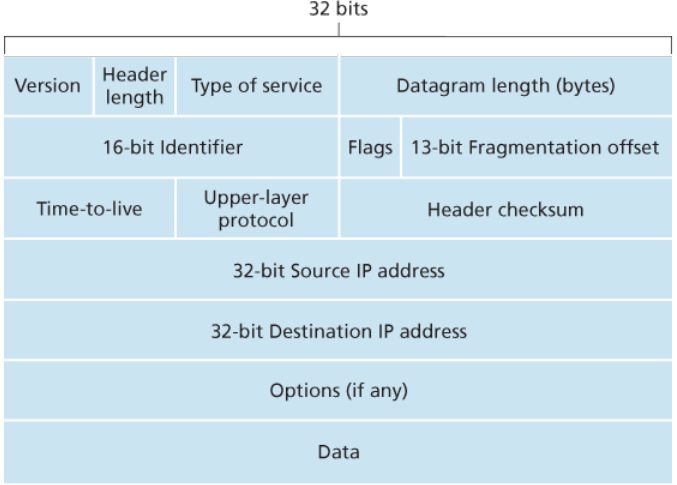
\includegraphics[width=\textwidth]{IPv4Datagram.png}
\caption{formato del datagramma IPv4}
\end{figure}
I campi nel datagramma IPv4 sono:
\begin{itemize}
\item Version number: questi 4 bit specificano la versione di IP utilizzata in modo che il router possa interpretare gli altri bit dell'header.
\item Header length: essendo che un header del datagramma pu\`o contenere informazioni di lunghezza variabile si deve notificare dove inizia il payload.
La lunghezza tipica \`e di 20 bytes.
\item Type of service: utilizzati per determinare degli utilizzi del datagramma come ECN o servizi real-time.
\item Datagram length: la lunghezza totale del datagramma misurata in bytes, \`e a 16 bit.
\item Identificatori, flags, segmentation offset.
\item Time-to-live: utilizzato per impedire che datagrammi circolino infinitamente. Questo campo \`e decrementato di $1$ ogni volta che un datagramma 
attraversa un router. Quando raggiunge zero deve essere droppato.
\item Protocol: tipicamente utilizzato quando il datagramma raggiunge la destinazione indica il tipo di protocollo di transport layer utilizzato. 6 per TCP
e 17 per UDP.
\item Header checksum: aiuta a individuare errori di bit in un ricevuto datagramma IP. Computato considerando 2 bytes nell'header come numeri e sommandoli 
tra di loro in complemento a 1. A causa del TLL viene ricomputato in ogni router. 
\item Source e destination IP addresses.
\item Options: opzionali causano differenze di processing per pacchetti diversi e segmenti di lunghezza diversa.
\item Data o payload: contiene il segmento del livello di trasporto. 
\end{itemize}
\subsection{IPv4 frammentazione del datagramma}
La massima quantit\`a di dati che un link pu\`o trasportare \`e detta maximum transmission unit (MTU) e determina un limite rigido per la dimensione massima
dei datagrammi. Essendo che da mittente e destinatario possono sussistere link con MTU diverse nascono dei problemi. Quando si deve inviare un datagramma
troppo grosso in un link con MTU troppo piccolo questo viene frammentato in due frame di livello di link pi\`u piccoli. Questi frammenti devono essere 
ricomposti prima di essere inviati al livello di trasporto. La deframmentazione avviene negli end-systems. Pertanto quando un host destinatario riceve dei
datagrammi deve determinare se questi sono frammenti di un datagramma originale. Deve anche determinare quando ha ricevuto l'ultimo frammento e come i 
frammenti debbano essere riuniti. Per far questo vengono utilizzate i campi di identification, flags e segmentation offset. Quando un datagramma \`e creato
il mittente lo marca con un identificatore  aumentato per ogni datagramma inviato. Quando tale datagramma viene frammentato ogni frammento possiede lo 
stesso identificatore. L'ultimo frammento ha un flag settato a 0 in modo da essere sicuri di aver ricevuto tutti i frammenti, il fragmentation offset \`e
utilizzato per ordinare e determinare se un frammento \`e mancante. 
\subsection{Indirizzamento IPv4}
Un host possiede tipicamente un unico link verso la rete e quando IP deve mandare un datagramma lo fa lungo quel link. Il limite tra l'host e il link fisico
viene chiamato interfaccia. Un router d'altra parte \`e connesso a numerosi link e pertanto possiede altrettante inferfacce. IP richiede che ogni 
interfaccia abbia il proprio indirizzo IP. Ogni indirizzo IP consiste di 32 bits scritti tipicamente nella dotted-decimal-notation, in cui ogni byte \`e 
scritto come decimale e separato dagli altri da un punto. Ogni interfaccia in ogni host e router deve possedere un IP univoco. Una porzione dell'indirizzo
viene scelta in base alla sottorete di appartenenza dell'interfaccia. Una rete che connette delle interfacce host con un interfaccia router \`e detta
sottorete (o rete IP). L'indirizzamento IP assegna un indirizzo alla sottorete $xxx.xxx.xxx.xxx/24$ dove $/24$ indica che i 24 bit pi\`u a sinistra detti
subnet mask definiscono l'indirizzo della sottorete e ogni host addizionale aggiunto alla sottorete avr\`a quei 24 bit uguali. Per determinare le subnets
si stacchi ogni interfaccia dal suo router o host creando delle reti isolate che vengono dette subnet. L'assegnazione di indirizzi IP dell'internet \`e
detta classless interdomain router (CIDR) che generalizza la cognizione di indirizzamento per le subnets. L'indirizzo IP a 32 bit \`e diviso in due 
parti e viene indicato con $a.b.c.d/x$ dove $x$ indica il numero di bit per la prima parte. Gli $x$ bit pi\`u significativi formano il prefisso o prefisso
di rete dell'indirizzo. Ad un'organizzazione vengono tipicamente assegnati IP contigui con lo stesso prefisso e sono gli unici bit considerati dai router
all'esterno dell'organizzazione. I rimanenti $32-x$ bits vengono utilizzati per fare forwarding sui pacchetti all'interno dell'organizzazione. Viene 
riservato l'indirizzo IP di broadcast 255.255.255.255 in cui il pacchetto viene duplicato in tutti gli host nella stessa sottorete. 
\subsubsection{Ottenere un blocco di indirizzi}
In ordine per ottenere un blocco di indirizzi IP per un'organizzazione si deve contattare un ISP che mette a disposizione indirizzi da un numero di 
indirizzi a sua disposizione ancora pi\`u grande. Lo fa aumentando la dimensione della subnet mask. L'interezza degli indirizzi IP \`e gestita dalla 
Internet corporationfor assigned names and numbers (ICANN) che si occupa di allocare gli indirizzi IP e di gestire i server DNS di root, assegna nomi di 
dominio e risolve dispute riguardo essi. Alloca indirizzi verso regristri locali che formano l'Address support organization dell'ICANN (ASO-ICANN) che 
gestiscono l'allocazione e la gestione di indirizzi all'interno della loro regione. 
\subsubsection{Ottenere un indirizzo IP per l'host: il Dynamic host configuration protocol}
Una volta che un'organizzazione ha ottenuto un blocco di indirizzi li pu\`o assegnare ad ogni interfaccia al suo interno. Gli indirizzi IP dei router sono
tipicamente configurati manualmente, mentre quelli degli host sono configurati attraverso il dinamic host configuration protocolo (DHCP) che permette ad un
host di ricevere un indirizzo IP automaticamente. L'host pu\`o ricevere lo stesso indirizzo IP ogni volta che si connette alla rete o ottenerne uno
temporaneo alla connessione. DHCP mette inoltre a disposizione all'host informazioni sul primo router (default gateway), la subnet mask e l'indirizzo del
server DNS locale. Questo protocollo \`e detto plug-and-play e zeroconf. DHCP \`e un protocollo client-server. Un client \`e tipicamente un nuovo host che
vuole ottenere informazioni per la configurazione di rete e un indirizzo IP per s\`e. Nel caso pi\`u semplice ogni subnet possiede un server DHCP. Se non 
\`e presente un DHCP relay agent che conosce la posizione del server DHCP per la rete \`e necessario. Per un nuovo host il protocollo DHCP \`e composto da
quattro fasi: 
\begin{itemize}
\item DHCP server discovery: il primo compito dell'host \`e quello di trovare il server DHCP ed \`e fatto attravreso un DHCP discover message che un client
invia attraverso un pacchetto UDP alla porta 67 con la broadcast definition dell'indirizzo IP e un questo host con indirizzo IP 0.0.0.0 l'host lo incapsula
in in frame di livello di link e fa un broadcast a tutti i nodi presenti nella sottorete.
\item DHCP server offer: il server che riceve il DHCP discovery message risponde al client con un DHCP offer message inviato attraverso il broadcast IP. 
Questo messaggio contiene il transacion ID del discover message, l'indirizzo IP proposto e l'IP lease time solitamente settato a ore o giorni. 
\item DHCP request: il client sceglie tra i server offer arrivatigli e risponde con un DHCP request message che fa echoing sui parametri di configurazione.
\item DHCP ACK: il server risponde al request message attraverso un DHCP ACK message che conferma i parametri richiesti. 
\end{itemize}
Una volta completati questi messaggi il client pu\`o utilizzare l'indirizzo IP consegnatogli. Se vuole continuare a utilizzarlo dopo la fine del lease time
DHCP mette a disposizione dei meccanismi per rinnovare l'indirizzo. Non si possono mantenere connessioni TCP se si sposta tra le sottoreti. 
\subsection{Network address translation (NAT)}
Il network addres translation viene utilizzato per facilitare la gestione di piccoli uffici o istallazioni casalinghe (SOHO) oltre a permettere di 
connettere pi\`u dispositivi all'internet. Un NAT-enabled router ha un'interfaccia parte della rete di casa. Tutte le interfacce in questa rete hanno la 
stessa subnet mask e lo spazio di indirizzo $/8$ \`e uno dei tre riservato per una rete privata o una realt\`a con reti private. Il NAT enable router non
sembra un router alla rete esterna ma viene considerato come come un singolo dispositivo con un singolo indirizzo IP, ovvero nasconde i dettagli della rete
casalinga al mondo esterno. Tutti questi indirizzi vengono ottenuti attraverso DHCP (dal server dell'ISP per il router e da quello del router per i 
dispositivi interni). Essendo che tutti i datagrammi che arrivano al router NAT hanno lo stesso indirizzo, per ottenere il destinatario corretto viene 
utilizzata una tabella di traduzione NAT e vengono inclusi i numeri di porta oltre agli indirizzi IP.
\subsection{IPv6}
I maggiori cambi nel formato del datagramma sono:
\begin{itemize}
\item Expanded addressing capabilities: la dimensione dell'inirizzo IP \`e aumentata da 32 a 128 bit. 
\item Un header di 40 byte fissi eliminando le opzioni in modo da permettere un router processing pi\`u veloce.
\item Flow labeling: in modo da marcare pacchetti per cui il mittente richiede una gestione speciale. 
\end{itemize}
\begin{figure}[h]
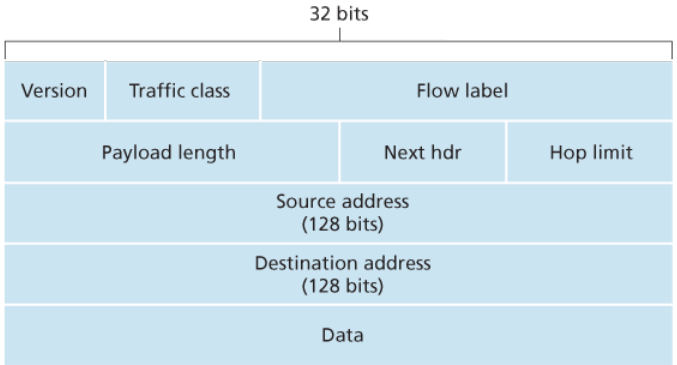
\includegraphics[width=\textwidth]{IPv6Datagram.png}
\caption{formato del datagramma IPv6}
\end{figure}
I seguenti campi sono definiti in IPv6:
\begin{itemize}
\item Version: il campo di 4 bit che indica la versione di IP utilizzata (con valore 6 per IPv6).
\item Traffic class: un campo a 8 bit come il TOS in IPv4.
\item Flow label: un campo a 20 bit che identifica datagrammi appartenenti ad un flow.
\item Lunghezza del payload: un unsigned integer che determina la lunghezza del payload del datagramma. 
\item Next header: identifica il protocollo del segmento contenuto.
\item Hop limit: questo valore \`e diminuito ogni volta che il datagramma attraversa un router e quando raggiunge zero il pacchetto viene eliminato.
\item Source and destination addresses: a 128 bit ognuno.
\item Data payload.
\end{itemize}
IPv6 a differenza di IPv4 non mette a disposizione un servizio di frammentazione: se un pacchetto \`e troppo grande lo droppa e invia al mittente un 
messaggio di ICMP che notifica che il pacchetto era troppo grande. Header checksum in quanto altri livelli lo compiono gi\`a e considerato ridondante. 
\subsubsection{Transizionare da IPv4 a IPv6}
Per effettuare la transizione da IPv4 a IPv6 viene utilizzato l'approccio del tunneling: quando un datagramma IPv6 trova un router ad IPv4 viene 
impacchettato in un nuovo datagramma IPv4 il nodo alla fine del tunneil IPv4 capisce che contiene un datagramma IPv6, lo estrae e lo forward. 
\section{Forwarding generalizzato e SDN}
Nel forwarding generalizzato una tabella match-plus-action generalizza la tabella di forwarding incontrata precedentemente. Questi dispositivi vengono 
riferiti come packet switch. La tabella in ogni packet switch \`e computata da un controller esterno. Ogni input in una tabella di match-plus-action 
chiamata flow table include:
\begin{itemize}
\item Un insieme di campi header ai quali un pacchetto in entrata sar\`a matchato utilizzando memoria TCAM, se non c'\`e nessun match il pacchetto pu\`o 
essere droppato o inviato al controller per ulteriore processing. 
\item Un insieme di contatori sono aggiornati mano a mano che i pacchetti sono matchati.
\item Un insieme di azioni da essere intraprese quando si trova un match. 
\end{itemize}
\subsection{Matching}
\begin{figure}[h]
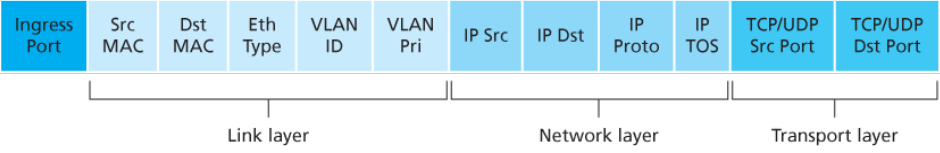
\includegraphics[width=\textwidth]{FlowTableEntry.png}
\caption{formato del datagramma IPv6}
\end{figure}
Si noti come l'astrazione fatta sul pacchetto perfette di accedere a dati provenienti da diversi livelli dello stack di rete. Le entries possono avere 
wildcards negli indirizzi IP e hanno una priorit\`a associata. 
\subsection{Action}
Dopo che avviene un match esiste una lista di zero o pi\`u azioni di processing da effettuare per quanto riguarda il pacchetto. Alcune delle pi\`u 
importanti sono:
\begin{itemize}
\item Forwarding: un pacchetto potrebbe essere inviato su una, alcune o tutte le porte di output o inviato al controller.
\item Dropping: il pacchetto viene droppato se non ci sono entries.
\item Modify-field: un campo del pacchetto viene modificato.
\end{itemize}
\chapter{Livello di rete: control plane}
\section{Introduzione}
Le tabelle di forwarding e di flow sono computate installate e mantenute secondo due approcci:
\begin{itemize}
\item Per-router control: un algoritmo di routing viene eseguito su ogni router della rete in cui sono contenute funzioni di routing e forwarding. Ogni 
router possiede una componente di routing che comunica con quella degli altri router per computare i valori della tabella di forwarding i protocolli di 
OSPF e BGP sono basati su questo approccio.
\item Logically centralized control: un controller centralizzato computa e distribuisce le tabelle di forwarding, permette di implementare numerose funzioni
attraverso una flow table. Il controller interagisce con ogni agente di controllo in ogni router attraverso un protocollo ben definito e non interagisce con
altri CA. 
\end{itemize}
\section{Algoritmi di routing}
Lo scopo di questi algoritmi \`e quello di determinare i cammini ottimi o routes da mittente e destinatario attraverso la rete di router. Un grafo \`e 
utilizzato per formulare questo problema in cui i nodi rappresentano router e gli archi i collegamenti tra di essi. Ogni arco ha un valore che rappresenta
il suo costo che riflette la lunghezza fisica del link, la sua velocit\`a di trasmissione e il costo economico. Per un arco $(x, y)$ si indica il costo 
attravreso $c(x, y)$, se il paio non appartiene al grafo $c(x, y)=+\infty$. L'obiettivo naturale per questo algoritmo \`e pertanto quello di trovare il 
cammino meno costoso tra due nodi. 
\begin{itemize}
\item Un algoritmo di routing centralizzato computa il cammino meno costoso utilizzando una conoscenza completa della rete, ovvero prende come input il 
grafo contenente tutti i nodi e tutti i link. Questi algoritmi sono detti algoritmi link-state (LS).
\item Un algoritmo di routing decentralizzato il calcolo del cammino meno costoso \`e effettuata in maniera distribuita dai router. Nessun nodo possiede 
conoscenza completa della rete, ma conosce unicamente i costi dei link a lui direttamente attaccati. Successivamente attraverso un processo iterativo di 
calcoli e di scambio di informazioni con altri nodi vicini il nodo calcola gradualmente il cammino meno costoso per un insieme di destinazioni. 
\end{itemize}
Gli algoritmi di routing si possono classificare anche in base al fatto che siano statici (dove routes cambiano raramente) o dinamici (dove routes cambiano
dinamicamente in maniera responsiva in base a cambi di topologia o di costo dei link: si ottenogno per esempio eseguendoli periodicamente. Un ulteriore 
metodo di classificazione si basa sul fatto se gli algoritmi sono load-sensitive o no in cui i costi dei link variano dinamicamente in base al livello di 
congestione della rete. 
\subsection{L'algoritmo di link state routing}
In modo da ottenere la topologia di rete e i costi dei link ogni nodo fa un broadcast link-state su tutti gli altri nodi della rete con ogni pacchetto 
contenente identit\`a e costo di ogni link del nodo. In questo modo tutti i nodi hanno una visione completa e globale della rete. L'algoritmo link-state di
routing \`e conosciuto come algoritmo di Dijkstra: questo algoritmo computa il cammino di costo minore da un nodo a tutti gli altri nodi nel pacchetto. 
Questo algoritmo ha la propriet\`a che alla fine della k-esima iterazione sono conosciuti i cammini minimi per k nodi, Si definisca $D(v)$ come il costo 
del cammino ottimo dal nodo di origine $u$ fino al nodo di destinazione $v$ di questa iterazione, $p(v)$ come il nodo genitore in questa esplorazione. $N'$
come il sottoinsieme dei nodi tali per cui il cammino ottimo \`e stato trovato. L'algoritmo consiste di una fase di inizializzazione e di un loop eseguito
per ogni nodo del grafo. 
\begin{figure}[h]
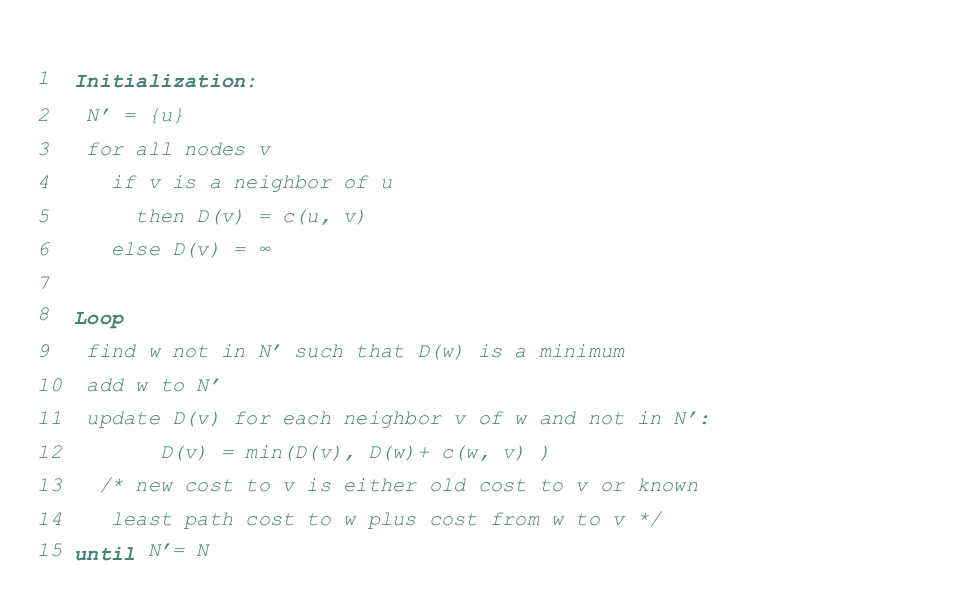
\includegraphics[width=\textwidth]{AlgoritmoDijkstra.png}
\caption{Algoritmo di Dijkstra}
\end{figure}
Quando l'algoritmo LS termina si ha per ogni nodo il suo predecessore e il cammino ottimo dal nodo di origine. La tabella di forwarding \`e costruita 
salvando per ogni destinazione il prossimo hop nel cammino ottimo. Questo algoritmo ha complessit\`a $O(n^2)$. 
\subsection{L'algoritmo di distance vector routing}
L'algoritmo di distance vector \`e iterativo, asincrono e distribuito. \`E distribuito nel senco che ogni nodo riceve informazioni da uno o pi\`u dei suoi
diretti vicini, svolge un calcolo e ritorna i dati ai vicini. \`E asincrono in quanto non richiede che i vicini operino in lockstep l'uno con l'altro ed \`e
self-terminating. Si consideri $d_x(y)$ il cammino ottimo da $x$ a $y$ e $v$ ogni vicino di $x$, allora secondo l'equazione di Bellman-Ford $d_x(y)=\min_v
\{c(x, v)+d_v(y)\}$. La soluzione a questa equazione d\`a le entries da mettere nella tabella di forwarding: si consideri $v*$ ogni nodo vicino che risolve
l'equazione allora la tabella deve indicarlo come prossimo hop per raggiungere infine $y$. Per trovare tali valori ogni nodo $x$ comincia con $D_x(y)$, una
stima del costo del cammino ottimo da s\`e stesso a qualsiasi nodo in $N$. Sia $D_x=\{D_x(y):y\in N\}$ il vettore delle distanze del nodo $x$, ovvero il
vettore della stima dei costi del cammino ottimo. Con l'algoritmo DV l'algoritmo di routing mantiene le seguenti informazioni:
\begin{itemize}
\item Per ogni vicino $v$, il costo $c(x, v)$.
\item Il vettore delle distanze di $x$, ovvero $D_x$.
\item Il vettore delle distanze di ogni suo vicino, ovvero $D_v$ per ogni vicino $v$.
\end{itemize}
Nell'algoritmo distribuito e asincrono ogni tanto ogni nodo manda una copia del suo vettore delle distanze ai suoi vicini che lo salvano e lo utilizzano
per aggiornare il proprio vettore delle distanze seguento l'equazione di Bellman-Ford: $D_x(y)=\min_v\{c(x, v)+D_v(y)\}$ per ogni nodo $y$ in $N$. Se il 
vettore delle distanze viene modificato nel passo di aggiornamento $x$ invia una copia ad ogni vicino. Se tutti i nodi contiunano a scambiarsi i vettori 
delle distanze in maniera asincrona ogni stima $D_x(y)$ converge a $d_x(y)$ il costo ottimo reale. 
\begin{figure}[h]
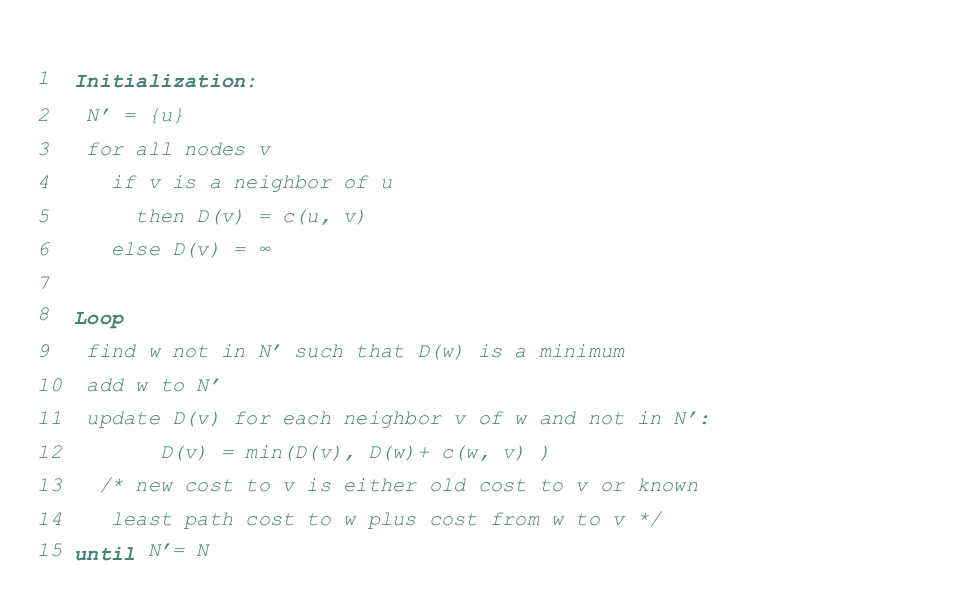
\includegraphics[width=\textwidth]{AlgoritmoDijkstra.png}
\caption{Algoritmo Distance Vector}
\end{figure}
Quello che interessa non \`e la lunghezza del cammino minimo, ma il vicino $v*$ obiettivo del prossimo hop, pertanto nelle righe 13-14 del codice si
prende il vicino che ha il valore minimo e lo si inserisce nella tabella. 
\subsubsection{Cambio di costo dei link e loro fallimento}
Quando un nodo che esegue l'algoritmo DV percepisce un cambio di costo in un link aggiorna il suo vettore delle distanze e se avviene un cambio nei percorsi
ottimi informa i suoi vicini. Questi aggiornamenti a causa della loro localit\`a possono causare dei routing loop che possono essere molto difficili da
risolvere, anche se poi verranno risolti. Questi problemi sono chiamati count-to-infinity problem. 
\subsubsection{Aggiungere poisoned revers}
Lo scenario appena descritto pu\`o essere evitato aggiungendo una poisoned reverse: se un nodo routa il pacchetto verso quello che gliel'ha inviato gli 
mente inviandogli che la sua distanza dalla destinazione finale \`e $\infty$ fino a che $z$ continuer\`a a fare routing verso la destinazione da tale nodo.
Credendo che non ci sia cammino il primo mittente cambier\`a cammino. Questa tecnica risolve il count-to-infinity problem unicamente se il loop accade su 
nodi vicini. 
\subsection{Confronto tra LS e DV}
Si indichi con $N$ il numero di nodi e con $E$ il numero di archi:
\begin{itemize}
\item Complessit\`a dei messaggi: essendo che LS richiede che ogni nodo conosca il costo di ogni link nella rete vengono richiesti $O(|V|+|E|)$ messaggi e 
il cambio di costo di un link deve essere comunicato a tutti i nodi. DV richiede uno scambio di messaggi unicamente tra vicini ad ogni iterazione il costo
di convergenza dipende da molti cammini. Il cambio di costo di un link causa una propagazione di messaggi unicamente se cambia un cammino ottimo.
\item Velocit\`a di convergenza: LS \`e un algoritmo in $O(|N|^2)$ messaggi che richiede $O(|V|+|E|)$ messaggi. L'algoritmo DV pu\`o convergere lentamente
e incontrare routing loop e il count-to-infinity problem.
\item Robustezza: i calcoli dei cammini sono separati in LS offrendo della robustezza mentre in DV dipendono dai calcoli dei vicini e pertanto se c'\`e un
malfunzionamento questo pu\`o diffondersi in tutta la rete.
\end{itemize}
\section{Intra-AS routing nell'internet: OSPF}
Il modello che considera l'internet come un omogeneo insieme di router che eseguono tutti lo stesso algoritmo \`e semplicistico per due ragioni:
\begin{itemize}
\item Scala: con la crescita del numero di router l'overhead necessaria a calcolare, comunicare e salvare le informazioni di routing diventa proibitiva. 
\item Autonomia amministrativa: l'internet \`e una rete di ISPs che possiedono la propria rete di routers. Queste ISP desiderano di operare in maniera pi\`u
autonoma possibile e amministrare la propria rete secondo il loro desiderio ma essere capaci di connettere la loro rete con le altre.
\end{itemize}
Entrambi questi problemi possono essere risolti organizzando i router in sistemi autonomi (ASs) consistenti di insiemi di router sotto lo stesso controllo
amministrativo, identificato globalmente dal suo autonomous system number (ASN), assegnati anche loro da ICANN. Router nello stesso AS eseguono lo stesso 
algoritmo di routing e possiedono informazioni gli uni degli altri. Questo algoritmo di routing \`e detto intra-autonomous system routing protocol. 
\subsection{Opend shortest path first (OSPF)}
Il routing OSPF e il suo simile IS-IS sono largamente utilizzati per le operazioni di routing per le intra-AS dell'internet. La parola Open indica che il 
protocollo \`e pubblicamente disponibile. Questo protocollo \`e un protocollo che usa flooding di informazioni di link-state e un algoritmo di cammino 
ottimo di Dijkstra. Ogni router costruisce una mappa topologica completa dell'intero sistema autonomo, ogni router successivamente esegue Dijkstra per 
determinare l'albero di cammino minimo per ogni sottorete con s\`e stesso come radice i costi di link sono configurati dal'amministratore di rete. Un router
fa un broadcast delle sue informazioni di link-state a tutti gli altri router ogni volta c'\`e un cambio in un link-state e periodicamente (almeno ogni 30
minuti). Questi messaggi sono trasportati direttamente da IP con un protocollo di livello pi\`u alto per OSPF che controlla se i link sono funzionali. 
Alcuni dei vantaggi di OSPF sono:
\begin{itemize}
\item Sicurezza: scambi tra router OSPF possono essere autenticati: solo trusted router possono partecipare nelle tabelle. Si pu\`o utilizzare una password
in plaintext o MD5.
\item Cammini ottimi multipli: quando esistono multipli cammini ottimi tutti possono essere utilizzati. 
\item Supporto integrato per unicast e multicast broadcasting: MOSPF usa il link database OSPF e aggiunge un nuovo tipo di avvertimento link state al 
meccanismo di broadcast.
\item Supporto per gerarchie all'interno di un singolo AS: L'AS viene separate in aree comunicanti attraverso area border router. Un'area \`e designata come
backbone per fare routing tra le vaire aree contiene tutti i router area border e anche altri. 
\end{itemize}
\section{Rounting tra ISPs: BGP}
Per fare routing tra host in diverse AS si rende necessario un protocollo di inter-autonomous system routing. Tutte le AS comunicanti devono eseguire lo 
stesso protocollo chiamato il Border Gateway protocol BGP. \`E un protocollo asincrono e decentralizzato con un algoritmo di routing DV. 
\subsection{Il roulo di BGP}
Se la destinazione di un pacchetto \`e esterna all'AS il pacchetto viene instradato verso prefissi CIDRized, con ognuno di essi rappresentanti una subnet o
un insieme di subnet. Pertanto un entry della tabella di forwarding avr\`a la forma $(x, I)$, con $x$ il prefisso e $I$ il numero di interfaccia di una 
delle interfacce del router. BGP mette a disposizione ad ogni router modi per:
\begin{itemize}
\item Ottenere informazioni di raggiungibilit\`a di prefissi da altri AS: permette ad ogni subnet di pubblicizzare la propria esistenza all'intero internet.
\item Determinare il cammino migliore per i prefissi.
\end{itemize}
\subsection{Pubblicizzare le informazioni di BGP route}
In un AS si distingue tra gateway router e router interni: i primi sono i router dell'AS che si connettono direttamente con router di altre AS. Per 
pubblicizzare la raggiungibilit\`a di un prefisso ogni AS manda un messaggio BGP agli AS vicini, che lo mandano a loro volta ai loro AS vicini indicando 
s\`e stessi come cammino intermedio. In BGP paia di router si scambiano informazioni attraverso una connessione TCP semi-permanente sulla porta 179. Ognuna
di queste in combinazione con il messaggi inviati \`e chiamata una connessione BGP. Una connessione BGP che attraversa pi\`u AS \`e detta esterna, 
altrimenti interna. Tipicamente si trova un eBGP per ogni link che connette due AS e un iBGP per ogni coppia di router all'interno dell'AS. I messaggi di 
raggiungibilit\`a sono pertanto propagati da una eBGP, successivamente distribuiti in tutta l'AS attraverso iBGP e poi ancora ad altre AS attraverso eBGP.
\subsection{Determinare il cammino ottimo}
Quando una connessione BGP pubblicizza un prefisso include ad esso vari attributi BGP formando una route. Due di questi attributi sono AS-PATH e NEXT-HOP.
Il primo contiene la lista di AS attraverso cui il messaggio di pubblicizzazione \`e passato, affinch\`e venga generato quando un prefisso \`e passato
ad un AS questo aggiunge ad esso il proprio ASN nella lista esistente in AS-PATH. Viene utilizzato anche per evitare loop di pubblicizzazione. L'attributo 
NEXT-HOP mette a disposizione il link tra i protocolli intra e inter AS e contiene l'indirizzo IP dell'interfaccia router che comincia l'AS-PATH.
\subsubsection{Hot potato routing}
In questo tipo di routing il cammino scelto \`e il cammino ottimo al router NEXT-HOP che comincia tale cammino. L'algoritmo pertanto opera in questa 
maniera:
\begin{itemize}
\item Apprende dal protocollo AS che una sottorete \`e raggiungibile da diversi gateways.
\item Usa il protocollo intra-AS per determinare il costo minimo a ciascuno di questi gateways.
\item Sceglie il gateway con il costo minore.
\item Determina dalla tabella di forwarding l'interfaccia che porta al gateway, inserisce $(prefisso, I)$ nella tabella. 
\end{itemize}
\subsubsection{Algoritmo di route-selection}
Per ogni dato prefisso di destinazione l'input di questo algoritmo \`e l'insieme di tutti i cammini verso quel prefisso che sono conosciute e accettate, se 
sono pi\`u di una invoca le seguenti regole di eliminazione fino a che ne rimane una sola:
\begin{itemize}
\item Un route \`e assegnato un valore di local preference come attributo. Le routes con il maggior valore di local preference sono selezionate.
\item Dalle routes rimanenti sono selezionate quelle con l'AS-PATH minore. 
\item Si seleziona dalle routes rimanenti utilizzando hot potato.
\item Se rimangono ancora pi\`u routes vengono utilizzati i BGP identifiers. 
\end{itemize}
\subsection{IP anycast}
BGP \`e utilizzato per implementare il servizio di IP anycast usato comunamente dai DNS. Viene utilizzato in quanto si \`e interessati a duplicare contenuti
in diversi server dispersi geograficamente e far accedere ogni utente al server pi\`u vicino. Durante la fase di configurazione dell'anycast una compagnia
assegna lo stesso indirizzo IP ai suoi server e usa BGP per pubblicizzare ognuno di questi. Quando un router riceve questi multipli li tratta come se 
mettessero a disposizione diverse routes per la stessa destinazione. 
\subsection{Politica di routing}
Il campdio della local preference \`e utilizzato per determinare delle zone protette dove non si devono svolgere operazioni di routing o per scegliere altri
cammini in modo da rispettare politiche dell'ISP. 
\section{The SDN control plane}
Si possono identificare quattro caratteristiche fondamentali di un'architettura SDN:
\begin{itemize}
\item Flow-based forwarding.
\item Separazione tra il data plane e il control plane con il primo hardware e il secondo software.
\item Funzioni di controllo di rete esterne agli switch data plane.
\item Rete programmabile. 
\end{itemize}
\subsection{Il control plane dell'SDN, controller e applicazioni di controllo di rete}
Il control plane dell'SDN si divide in due componenti principali: un controller SDN e le applicazioni di controllo di rete. Le funzionalit\`a di un 
controller di possono dividere in tre categorie:
\begin{itemize}
\item Un livello di comunicazione tra il controller e i dispositivi connessi alla rete attraverso un protocollo conosciuto come l'interfaccia "southbound"
del controller.
\item Un livello di gestione dello stato per tutta la rete in quanto decisioni prese dal controller richiedono informazioni riguardo tutta la rete. 
\item Un interfaccia verso le applcazioni di controllo di rete detta anche interfaccia "northbound" in modo di permettere a funzioni di leggere e scrivere
all'interno del livello di gestione di stato della rete. 
\end{itemize}
Il controller \`e logicamente centralizzato ma in realt\`a \`e costituito da diversi server con database e algoritmi distribuiti. 
\subsection{Il protocollo OpenFlow}
Il protocollo OpenFlow opera tra il controller e unp switch controllato da SDN, opera attraverso TCP con porta 6653. Tra i messaggi inviati dal controller
allo switch figurano:
\begin{itemize}
\item Configurazione: per fare query e settare i parametri di configurazione di uno switch.
\item Modifica di stato: per aggiungere o eliminare entries nelle tabelle di flow o per cambiare propriet\`a di porte.
\item Lettura di stato: utilizzato per collezionare statistiche e contatori dalle porte e tabelle dello switch. 
\item Invio di pacchetto: utilizzato per mandare uno specifico pacchetto ad una porta specifica allo switch il messaggio contiene il pacchetto che deve 
essere mandato come suo payload.
\end{itemize}
Tra i messaggi inviati dallo switch al controller figurano:
\begin{itemize}
\item Flow rimosso: informa il controller che un entry nella tabella di flow \`e stata rimossa. 
\item Status di porta: informa il controller in un cambio di status in una porta.
\item Packet-in: manda al controller il pacchetto senza entry nella tabella di flow. 
\end{itemize}
\section{ICMP il protocollo di internet control message}
Il protocollo di internet control message \`e utilizzato da host e router per comunicare informazioni di livello di rete tra di loro. L'utilizzo pi\`u comune \`e il report degli errori.  Architetturalmente si trova appena
sopra IP in quanto messaggi ICMP sono spostati come payload di IP. Quando un host riceve un datagramma IP con ICMP specificato come il protocollo di livello superiore (con numero 1) fa demultiplexing a 
ICMP. I messaggi ICMP hanno un tipo e in campo di codice e congengono l'header e i primi 8 bytes del datagramma IP che ha causato la generazione del messaggio in modo che il mittente pu\`o determinare
quale datagramma ha generato l'errore.  
\begin{figure}[h]
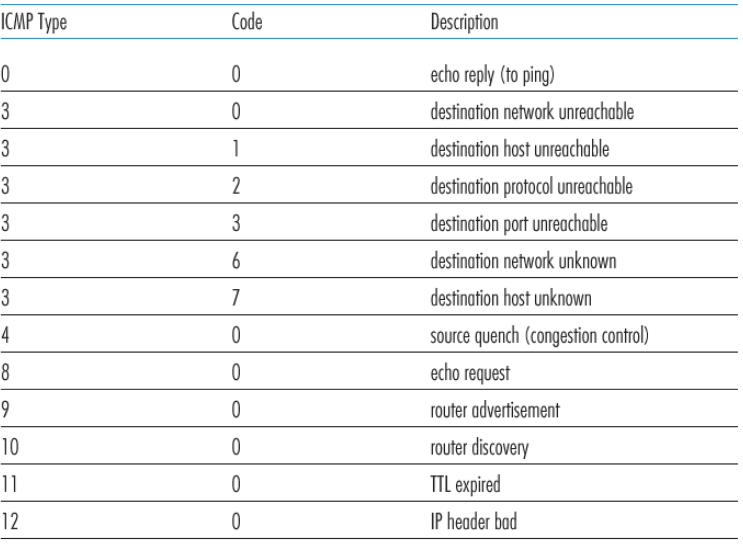
\includegraphics[width=\textwidth]{ICMPValues.png}
\caption{Tipi di messaggio ICMP}
\end{figure}
Traceroute utilizza questi messaggi generando pacchetti UDP con TLL incrementale su una porta strana fino a che arriva a ricevere un messaggio ICMP di tipo 3 con codice 3.
\section{Gestione della rete e SNMP}
La gestione della rete include distribuzione, integrazione e coordinazione dell'hardware, software e elementi umani per monitorare, testare, sondare, configurare, analizzare, valutare e controllare la rete e le
risorse elementari in tempo reale, con prestazioni operazionali e servizio di qualit\`a ad un costo ragionevole. 
\subsection{Il framework per la gestione della rete}
Le componenti chiave della gestione di rete sono:
\begin{itemize}
\item Il managing server, un'applicazione con un umano nel ciclo che viene eseguita nel centro delle operazioni di rete (NOC) che controlla la collezione, processing, analisi e visione di attivit\`a della gestione di 
rete. \`E qui che le azioni sono iniziate per controllare il comportamento della rete.
\item Un managing device, un equipaggiamento di rete che si trova sulla rete gestita che gestisce dei managed objects che sono strumenti hardware e la configurazione dei loro parametri.
\item Un management information base (MIB) che raccoglie le informazioni di ogni managed object e le mette a disposizione del managing server. Questi parametri sono specificati in SMI (structure of 
management information). 
\item Il network management agent \`e il processo che comunica con il managing server.
\item Il network management protocol che viene eseguito tra il managing server e i managed device in modo da permettere la comunicazione e le query tra i due. 
\end{itemize}
\subsection{Il simple network management protocol (SNMP)}
SNMP \`e un protocollo di livello applicativo utilizzato per trasportare controllo di gestione della rete e informazioni  tra un managing server e un agente che esegue al suo posto. L'utilizzo pi\`u comune \`e in
modalit\`a request-response in cui un managing server SNMP invia una richiesta ad un agente SNMP che la riceve, svolge qualche azione e invia una risposta alla richiesta. Le richieste sono utilizzate per query o 
per modificare oggetti MIB. Viene anche utilizzato per mandare trap message al managing server per notificarlo di situazioni eccezionali. Vengono definiti sette tipi di messaggi detti protocol data units (PDUs).
\begin{itemize}
\item I messaggi \emph{GetRequest, GetNextRequest} e \emph{GetBulkRequest} sono inviate dal managing server per richiedere valori di uno o pi\`u oggetti MIB al managed device dell'agente. Gli oggetti 
richiesti sono specificati nella porzione di variable binding. L'agente risponde con una PDU di risposta che contiene gli identificatori degli oggetti e i valori associati.
\item Il PDU \emph{SetRequest} \`e utilizzato dal managing server per settare i valori di uno o pi\`u oggetti MIB in un managed device. UN agente risponde con un PDU di risposta con lo status di errore
noError per confermare che il valore \`e stato settato. 
\item Il PDU \emph{InformationRequest} \`e utilizzato dal managing server per notificare un altro managing server di informaizoni MIB che sono remote al server destinatario.
\item Il PDI \emph{Response} \`e tipicamente mandato da un managed defivse in risposta ad un request message ritornando le informazioni richieste.
\item Il tipo finale \`e il trap message, sono generati asincronamente, ovvero non sono generati in risposta a richieste ma in risposta a eventi per i quali il server richiede notifica. 
\end{itemize}
Sono tipicamente trasmessi attraverso UDP.
\begin{figure}[h]
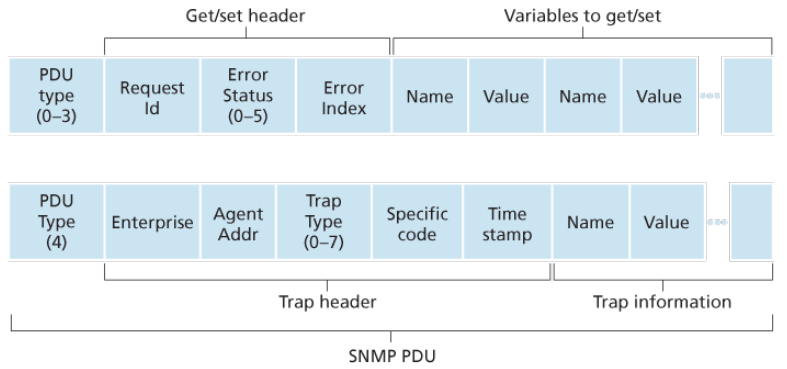
\includegraphics[width=\textwidth]{SNMPPDUFormato.png}
\caption{Formato di un PDU SNMP}
\end{figure}
\chapter{Il livello di link e LANs}
Esistono due tipi di canali a livello di link: il primo tipo sono i canali broadcast che connettono multipli host e rendono necessario un access medium protocol; il secondo tipo \`e il link di comunicazione punto a 
punto.
\section{Introduzione}
Si indica un oggetto che esegue un protocollo di livello di link come ad un nodo che includono host, router, switches e WIFI access point. Ci si riferisce ai canali di comunicazione che connettono i nodi adiacenti 
come links. In modo che un datagramma sia trasferito da un host source a uno di destinazione si deve muovere lungo ognuno dei link individuali nel cammino. Su un dato link un modo trasmettitore incapsula
il datagramma in un frame di livello di link e lo trasmette nel link. 
\subsection{Servizi messi a disposizione}
Nonostante il servizio base di ogni livello di link \`e di spostare un datagramma da un nodo all'adiacente lungo un singolo link di comunicazione ci sono altre funzionalit\`a che dipendono dal protocollo:
\begin{itemize}
\item Framing: quasi tutti i protocolli di livello di link incapsulano ogni datagramma di livello di rete in un frame prima di trasmetterlo lungo il link. Un frame consiste in un campo di dati dove si trova il payload e 
un numero di campi di header. 
\item Link access: un protocollo di medium access control (MAC) specifica le regole secondo cui un frame \`e trasmesso lungo il link. Il protocollo diventa naturalmente pi\`u complesso per i canali broadcast in 
quanto coordina la trasmissione dei frame ai vari nodi.
\item Reliable deliver: quando il protocollo la mette a disposizione garantisce di muovere ogni datagramma lungo il link senza errori.  Similarmente  a TCP pu\`o essere ottenuto con ACK e ritrasmissioni. Questo
si fa nel tentativo di correggere l'errore localmente. Maggiormente diffuso per i link wireless.
\item Error detection and correction: l'hardware del livello di link in un nodo ricevente potrebbe flippare erroneamente un bit. In quanto sarebbe inutile continuare l'invio del pacchetto molti protocolli mettono
a disposizioni metodi per individuare tali errori. \`E ottenuto attraverso l'aggiunta di bit per questo scopo attraverso tecniche pi\`u sofisticate dei livelli superiori e implementazione hardware. Per la correzione di
tali errori si rende necessario capire in quali bit \`e avvenuto l'errore.  
\end{itemize}
\subsection{Implementazione del livello di link}
Nei router \`e implementato nelle line cards. Per la maggior parte il livello di link \`e implementato in un network adapter (network interface card o NIC), nel cui cuore si trova il controller del livello di link, un chip
special purpose che implementa molti dei servizi. Dal lato mittente il controller prende un datagramma che \`e stato creato e salvato nella memoria dell'host dai livelli superiori, lo incapsula in un frame 
riempiendo i campi dell'header e lo trasmette nel link di comunicazione attraverso il protocollo di link-access. Dal lato del ricevente un controller riceve un frame ed estrae il datagramma del livello di rete. Se 
esegue error detection il mittente setta i bits necessari nell'header e il ricevente esegue l'error detection. Le parti implementate in software mettono a disposizioni funzionalit\`a di alto livello come assemblare
indirizzamento di livello di link e attivare il controller hardware. Dal lato del ricevente il software risponde ad un controller interrupt gestisce le condizioni di errore i passa il datagramma ai livelli successivi. 
\section{Tecniche di individuazione e correzione errori}
Al nodo inviante i dati D che devono essere protetti da errori sono aumentati con bit di individuazione e correzione errori (EDC), tali dati sono composti dal datagramma, informazioni di indirizzamento di livello 
di link, numeri di sequenza e altri campi nel frame header. Sia D che EDC sono inviati al nodo ricevente in un frame. Al nodo ricevente una sequenza di bit D' e EDC' sono ricevuti. A causa di errori i primi e i 
secondi potrebbero variare. Il ricevente deve essere in grado di determinare se sono diversi. Queste tecniche non sono perfette. Tecniche pi\`u sofisticate richiedono overhead maggiori.
\subsection{Parity checks}
Questo metodo di individuazione errori consiste nell'utilizzo di un singolo parity bit. Si supponga che l'informazione da inviare D ha $d$ bit. In un even parity scheme il mittente include un bit aggiuntivo e 
sceglie il suo valore tale che il numero totale di uni nei bit $d+1$ \`e pari. Il ricevente deve solo contare i numeri di uni nei $d+1$ bit. Se \`e dispari c'\`e un errore, altrimenti no. Se succede un numero pari di bit 
errors l'errore non viene individuato. Si pu\`o fare una generalizzazione bidimensionale in cui i $d$ bit sono divisi in $i$ righe e $j$ colonne. Un valore di parity \`e computato per ogni riga e per ogni colonna. I 
risultanti $i+j+1$ parity bit sono inclusi nel campo appropriato. Con questo schema bidimensionale quando accade un errore la parity sia della colonna che della riga sono sbagliate e pertanto si pu\`o 
identificare il bit singolo sbagliato e correggerlo (se c'\`e un singolo errore). L'abilit\`a per un ricevente di individuare e correggere errori \`e conosciuta come forward error correction (FEC). 
\subsection{Checksumming methods}
Questo metodo di individuazione consiste nel trattare i $d$ bit di dati come una sequenza di $k$-bit integer. Un semplice metodo consiste nel sommare questi interi e utilizzare tale somma come i bit per l'error
detection. L'internet checksum \`e basato su questo approccio. 
\subsection{Cyclic redundancy check (CRC)}
Questa tecnica utilizzata in larga scala \`e basata sui codici di cyclic redundancy check. Sono conosciuti come codici polinomiali in quanto \`e possibile considerare la stringa di bit come un polinomio i cui 
coefficienti sono i valori 0 e 1 con operazioni sulla stringa di bit interpretate come aritmetica polinomiale. Si consideri il dato D di $d$ bit che il mittente vuole inviare. Il mittente e il ricevente devono prima 
mettersi d'accordo su un pattern a $r+1$ bit conosciuto come un generatore che si denota con G. Si impone che il bit pi\`u significativo di G sia 1. Per un dato il mittente sceglie $r$ bit addizionali $R$ e li 
aggiunge a D in modo che il pattern $d+r$ interpretato come un numero binario sia esattamente divisibile da G utilizzando l'aritmetica modulo 2. Il processo di controllo errori consiste nella divisione da parte 
del ricevente dei $d+r$ bit ricevuti con G. Se il rimanente \`e non zero il ricevente sa che c'\`e stato un errore, altrimenti i dati sono accettati come corretti. Utilizzando l'aritmetica modulo due senza riporti
sottrazione e addizione si computano attraverso XOR, mentre moltiplicazione e divisione attraverso shift. Pertanto dati D e R la quantit\`a $D\cdot 2r XOR R$ contiene i $d+R$ bit. Si deve pertanto capire come
il mittente computa $R$. Considerando l'equazione precedente si pu\`o calcolare $R=D2r\mod G$. Gli standard CRC possono individuare burst errors di meno di $r+1$ bit. Sotto certe assunzioni possono 
individuare i burst error maggiori con probabilit\`a $1-0.5r$, possono individuare ogni numero dispari di errori. 
\section{Access links multipli e protocolli}
Un link point-to-point consiste di un singolo mittente a un capo e in singolo ricevente all'altro. Molti protocolli di livello di link sono stati costruiti per questo scopo. Un altro tipo di link \`e un link broadcast che 
pu\`o avere multipli mittenti e riceventi tutti connessi allo stesso condiviso canale broadcast. Quando un nodo trasmette un frame tutti i nodi connessi al link ne ricevono una copia. Ne sono un esempio 
ethernet e wireless LAN. Si vedr\`a come gestire il problema del multiplo accesso. Vengono pertanto creati protocolli di accesso multiplo secondo i quali i nodi regolano la loro trasmissione sul canale condiviso.
Essendo che tutti i nodi sono capaci di trasmettere frame possono inviarli allo stesso momento e i frame collidono a tutti i riceventi. Quando c'\`e una collisione i segnali dei frames si ingarbugliano tra di loro. 
Diventa pertanto necessario coordinare la trasmissione dei nodi attivi, lavoro svolto dal protocollo di accesso multiplo. Questi protocolli si possono dividere in channel partitioning, random access e taking-
turns. Questi protocolli per un canale con tasso di trasmissione di $R\frac{bits}{second}$ dovrebbero:
\begin{itemize}
\item Quando solo un nodo deve trasmettere dei dati il suo throughput deve essere $R$.
\item Quando $M$ nodi devono trasmettere ognuno di essi deve avere un throughput di $\frac{R}{M}$ come tasso di trasmissione medio.
\item Il protocollo \`e decentralizzato.
\item Il protocollo \`e semplice e poco costoso da implementare.
\end{itemize}
\subsection{Protocolli di channel partitioning}
Time division-multiplexing (TDM) e frequency-division multiplexing (FDM) sono due tecniche utilizzate per partizionare la bandwidth di un canale broadcast tra tutti i nodi che condividono il canale. TDM divide
il tempo in time frames e divide ogni time frame in time slots pari al numero di nodi nel canale. Ogni time slot \`e assegnato ad uno dei nodi. Ogniqualvolta un nodo deve trasmettere un pacchetto lo trasmette
durante il suo assegnato time slot nel corrente TDM frame. Le dimensioni degli slot sono decise in modo che un singolo pacchetto possa essere trasmesso durante uno slot time.   FDM divide il canale in 
frequenze diverse invece di time slots e assegna una frequenza ad ogni nodo. Entrambi eliminano le collisioni e sono perfettamente fair, ma un nodo deve aspettare sempre il suo momento anche se \`e l'unico 
che deve inviare un pacchetto. Un terzo protocollo di questo tipo \`e il code division multiple access (CDMA) che assegna un codice diverso ad ogni nodo che lo utilizza per codificare i dati che invia. Se i codici
sono scelti accuratamente i nodi diversi possono trasmettere simultaneamente e avere i destinatari ricevere correttamente i dati codificati se conosce il codice del mittente. 
\subsection{Random access protocols}
In questi protocolli un nodo trasmette al tasso pieno. Quando c'\`e una collisione tutti i nodi coinvolti aspettano un tempo randomico prima di ritrasmettere il pacchetto. 
\subsubsection{Slotted ALOHA}
Si assuma che tutti i frame consistano di $L$ bit, il tempo \`e diviso in slot di dimensione $\frac{L}{R}$, i nodi cominciano a trasmettere frames solo all'inizio degli slot, sono sincronizzati in modo che ogni nodo
sa quando lo slot comincia, se due o pi\`u frame collidono in uno slot tutti i nodi individuano la collisione prima che lo slot finisce. Sia $p$ una probabilit\`a, le operazioni dello slotted ALOHA in ogni nodo sono:
\begin{itemize}
\item Quando un nodo ha un nuovo frame da inviare aspetta fino all'inizio del prossimo e trasmette l'intero frame nello slot.
\item Se non c'\`e collisione il nodo \`e stato trasmesso con successo.
\item Se c'\`e collisione il nodo la individua prima della fine dello slot e ritrasmette il frame in ogni slot seguente con probabilit\`a $p$ fino a che il frame \`e trasmesso senza collisione. La propriet\`a di un nodo
\`e indipendente da quella negli altri.
\end{itemize}
A differenza del channel partitioning permette ad un nodo di trasmettere continuamente al tasso pieno ed \`e altamente decentralizzato, anche se richiede una sincronizzazione degli slot. Quando c'\`e una 
collisione \`e possibile perdere uno slot, alcuni slot possono rimanere vuoti. Uno slot non sprecato si dice successful. L'efficienza di uno slotted multiple accesso protocol \`e definita come la frazione di slots
successful nella long-run, Supponendo che ogni nodo provi a trasmettere un frame in ogni slot con probabilit\`a $p$ e che ci siano $N$ nodi.  La probabilit\`a che un dato slot sia successful \`e la probabilit\`a che
un nodo trasmetta: $p\frac{1-p}{N-1}$. La probabilit\`a che un nodo abbia un successo \`e $Np\frac{1-p}{N-1}$ che \`e l'efficienza del protocollo slotted ALOHA. Per ottimizzare l'efficienza si deve trovare la
probabilit\`a $p*$ per cui quel valore \`e massimo e per un grande numero di nodi si prende il limite a infinito di $Np*\frac{1-p*}{N-1}$. La massima efficienza \`e  $\frac{1}{e}$, ovvero al meglio solo il $37\%$ 
degli slot fa del lavoro utile, lo stesso numero di slot rimangono vuoti e nel $26\%$ ci sono collisioni. 
\subsubsection{ALOHA}
In ALOHA puro non esistono gli slot: quando arriva un frame il mittente lo trasmette immediatamente. Se c'\`e una collisione il nodo lo ritrasmette immediatamente con probabilit\`a $p$ o aspetta per un 
frame transmission time e ripete. Per determinare la massima efficienza ci si concentri su un nodo individuale e il frame transmission time un unit\`a di tempo. Ad ogni momento la probabilit\`a che un nodo 
stia trasmettendo un frame \`e $p$. Si supponga che inizi la trasmissione a tempo $t_0$, pertanto nessun altro nodo pu\`o iniziare a  trasmettere nell'intervallo $[t_0-1, t_0]$ in quanto le trasmissioni si 
sovrapporrebbero. La probabilit\`a di una trasmissione con successo \`e $p\frac{1-p}{2(N-1)}$. Si trova che la massima efficienza \`e $\frac{1}{2e}$, la met\`a dello slotted ALOHA, il prezzo per un protocollo
completamente decentralizzato. 
\subsubsection{Carrier Sense Multiple Access (CSMA)}
Si dice carrier sensing il fatto che un nodo ascolta il canale prima di trasmettere. Se un frame sta venendo trasmesso aspetta fino a che non individua nessuna trasmissione per un breve periodo prima di 
cominciare la trasmissione. Si dice collision detection il fatto che un nodo trasmettente ascolta il canale mentre trasmette e se individua che un altro nodo sta trasmettendo blocca la sua trasmissione e aspetta
un randomico tempo prima di ripetere il processo di sense-and-transmit-when-idle. Queste regole sono caratteristiche della famiglia dei carrier sense multiple access (CSMA) e CSMA con collision detection
(CSMA/CD). Questi protocolli non evitano completamente collisioni a causa del channel propagation delay. La probabilit\`a di collisioni \`e direttamente proporzionale a questo ritardo.
\subsubsection{Carrier sense multiple access con collision detection (CSMA/CD)}
Quando un nodo svolge la collision detection smette la trasmissione appena individua una collisione. Aumenta le prestazioni in quanto riduce i frame inutili trasmessi. Le operazioni di questo protocollo sono:
\begin{itemize}
\item L'adattatore riceve un datagramma dal livello di rete, prepara il frame e lo mette nel buffer.
\item Se l'adattatore percepisce che il canale \`e in quiete comincia la trasmissione del frame. Se percepisce che \`e occupato aspetta fino a che entra in quiete.
\item Mentre trasmette l'adattatore monitora per la presenza di segnali che arrivano da altri adattatori nel canale.
\item Se l'adattatore trasmette l'intero frame senza percepire nessun'altra trasmissione termina il frame, altrimenti fa abort della trasmissione.
\item Dopo l'abort l'adattatore aspetta un tempo randomico e ritorna al secondo passo.
\end{itemize}
La necessit\`a di aspettare un tempo randomico \`e per impedire collisioni infinite. La dimensione dell'intervallo \`e determinata dall'algoritmo di binary exponential backoff. Quando si trasmette un frame che ha
gi\`a avuto $n$ collisioni un nodo sceglie un valore di $K$ a caso tra $[0,2n-1]$, che pertanto aumenta con le collisioni. Pertanto la dimensione dell'insieme in cui $K$ \`e scelto cresce esponenzialmente con il 
numero di collisioni. Non c'\`e alcuna assicurazione sul mantenimento dell'ordine dei frame. 
\paragraph{Efficienza CSMA/CD}
Quando c'\`e un unico frame da inviare utilizza il pieno tasso di trasmissione del canale. Si definisce l'efficienza di questo protocollo come la frazione di tempo durante i quali i frame sono trasmessi sul canale
senza collisioni quando c'\`e un gran numero di nodi presenti. Sia $d_{prop}$ il tempo massimo che impiega il segnale a propagarsi tra due adattatori e $d_{trans}$ il tempo per trasmettere un frame di 
dimensione massima. $Efficiency = 11 + 5\frac{d_{prop}}{d_{trans}}$. 
\subsection{Protocolli taking-turn}
Esistono diverse variet\`a di questi protocolli, uno dei quali \`e il protocollo polling: in questo protocollo richiede che uno dei nodi sia un master node che abilita la comunicazione di ogni nodo in round-robin. In particolare manda un 
messaggio ad un nodo dicendo che pu\`o trasmettere fino ad un massimo numero di frame un nodo alla volta per ogni nodo. Elimina le collisioni ed empty slots ma introduce un ritardo di polling (il tempo
richiesto per notificare un nodo) e se il master node diventa inoperativo l'intero canale fallisce. Un secondo di questo tipo di protocolli \`e il token passing protocollo: un piccolo frame special purpose noto come
token \`e scambiato tra i nodi in un ordine prefissato. Quando un nodo lo riceve lo trasmette se ha dei frame da trasmettere, altrimenti lo passa al prossimo. Il numero di frame che si possono mandare in una 
sessione \`e limitato. 
\subsection{DOCSIS: il protocollo di livello di link per cable internet access}
Un cable network tipicamente connette diverse migliaia di cable modems residenziali ad un cable modem termination system. Il data over cable service interface specification (DOCSIS) specifica l'architettura
del cable data network e il suo protocollo. Utilizza FDM per dividere segmenti di rete  in downstream e upstream in frequenze multiple. Ogni canale downstream \`e largo $6MHz$ con un massimo throughput 
di $40Mbps$ per canale e $30$ per l'upstream con una larghezza di $6.4MHz$.  Ognuno di questi canali \`e un canale broadcast.  I frame trasmessi sul canale downstream sono ricevuti da tutti i cable modems
che ricevono quel canale ed essendoci un unico CMTS non c'\`e il problema del multiple access che si trova nella direzione dell'upstream. Ogni canale upstream \`e diviso in intervalli di tempo che contengono 
una sequenza di mini slot durante i quali i cable modems possono trasmettere al CMTS che esplicitamente garantisce il permesso a individui di trasmettere durante specifici mini-slots. Questo avviene grazie un 
messaggio di controllo MAP sul canale di downstream per specificare quale cable modem pu\`o trasmettere durante quale mini-slot. Il CMTS sa quali modem hanno dati da inviare grazie al fatto che questi 
ultimi inviano mini-slot-request durante uno speciale insieme di intervalli mini-slot dedicati per questo scopo. Questi messaggi sono trasmessi in maniera random access. I modem inferiscono le collisioni se 
non ricevono risposta e utilizzano exponential backoff per differire la ritrasmissione. 
\section{Switched local area networks}
In switched local area networks ci sono degli switches che operano al livello di link e switchano frames e non riconoscono indirizzi a livello di rete. 
\subsection{Indirizzamento livello di rete e ARP}
Host e router possiedono indirizzi a livello di link. 
\subsubsection{Indirizzi MAC}
Non sono host e router a possedere questi indirizzi ma i loro adattatori. Gli switch di livello di link non hanno indirizzi associati con le loro interfacce in quanto il loro lavoro \`e di trasportare datagrammi tra 
host e router. Un indirizzo di livello di link \`e chiamato indirizzo MAC. Per la maggior parte delle LAN \`e lungo 6 bytes tipicamente  espressi utilizzano la notazione esadecimale con ogni byte espresso come una 
coppia di numeri esadecimali. \`E possibile cambiare un indirizzo MAC via software. L'indirizzo MAC \`e univoco grazie alla gestione di IEEE: quando una compagna vuole creare adattatori compra un insieme di
indirizzi consistente di $2^{24}$ per una tassa nominale. IEEE alloca l'insieme fissando i primi 24 bit dell'indirizzo MAC e lasciando che la compagnia crei le combinazioni univoche per ogni adattatore. Non ha
una struttura gerarchica e non \`e dipendente dalla locazione geografica. Quando un adattatore vuole mandare un frame ad un destinatario inserisce l'indirizzo MAC del secondo nel frame e invia il frame nella 
LAN. Uno switch occasionalmente potrebbe inoltrare un pacchetto di tipo broadcast, pertanto un adattatore potrebbe ricevere un frame non per lui e deve controllare se l'indirizzo MAC di destinazione coincide con il suo. Se cos\`i non \`e scarta il frame, altrimenti estrae il datagramma e invia il pacchetto al livello di rete. Se si vuole inviare un messaggio a tutti gli altri adattatori nella LAN si utilizza l'indirizzo MAC broadcast  che consiste di una stringa di 48 uni consecutivi. 
\subsubsection{Address resolution protocol (ARP)}
Siccome ci sono sia indirizzi di livello di rete e indirizzi di livello di link si rende necessario tradurre da uno all'altro. Nell'internet questo lavoro \`e svolto da ARP. Un modulo ARP nell'host mittente prende ogni 
indirizzo IP nella stessa LAN come input e ritorna il corrispondente indirizzo MAC. Ogni host e router possiede una tabella ARP in memoria che contiene la mappatura tra IP e MAC e un valore di time-to-live che
indica quando ogni mappatura sar\`a eliminata dalla tabella, tipicamente 20 minuti. Se la tabella non possiede l'entry per la destinazione il mittente utilizza il protocollo ARP: costruisce un pacchetto speciale
chiamato pacchetto ARP che ha vari campi tra cui mittente e destinatario indirizzi IP e MAC. Sia richiesta che risposta hanno lo stesso formato. Lo scopo di un pacchetto ARP di query \`e di fare query su tutti gli 
altri host e router nella sottorete per determinare l'indirizzo MAC corrispondete all'indirizzo IP che sta venendo risolto e utilizzer\`a il broadcast MAC address. Ognuno dei moduli ARP che lo ricevono fa un 
controllo per verificare se l'indirizzo IP corrisponde e quello con il match risponde con un pacchetto ARP di risposta con la mappatura desiderata. Il mittente pu\`o aggiornare la sua tabella e inviare il frame. 
\subsubsection{Inviare un datagramma fuori dalla sottorete}
Quando si vogliono inviare datagrammi in un'altra sottorete si indica come indirizzo MAC quello del first hop router che lo porta fuori dalla rete che lo porta nel suo livello di trasporto, attraverso l'IP e ARP
determina l'indirizzo MAC del destinatario e lo inserisce nel nuovo frame creato. 
\subsection{Ethernet}
Una rete che utilizza ethernet consiste di host e router connessi con una topologia a stella ad uno switch. 
\subsubsection{Struttura di un frame ethernet}
\begin{figure}[h]
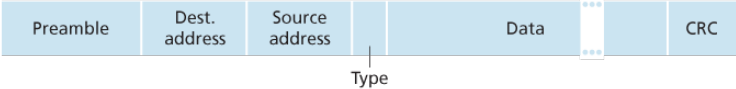
\includegraphics[width=\textwidth]{Pictures/EthernetFrame.png}
\caption{Struttura di un frame ethernet}
\end{figure}
I campi di un frame ethernet sono:
\begin{itemize}
\item Data field (46 - 1500 bytes): trasporta il datagramma IP, ethernet ha una MTU (maximum transmission unit) di 1500 bytes. Se il datagramma supera questa dimensione deve essere frammentato e se ha
una dimensione minore di 46 bytes deve essere riempito per raggiungere quel valori.
\item Destination address (6 bytes): contiene l'indirizzo MAC dell'adattatore di destinazione che scarter\`a tutti i frame con un MAC diverso dal proprio.
\item Source address (6 bytes): contiene l'indirizzo MAC dell'origine del frame.
\item Type field (2 bytes): permette a ethernet di fare multiplex al protocollo del livello di rete (in modo da riconoscere quello utilizzato).
\item Cyclic redundancy check (4 bytes): utilizzato per controllare errori.
\item Preamble (8 bytes): i primi 7 bytes hanno un valore di $10101010$, l'ultimo di $10101011$. I primi byte servono a svegliare l'adattatore ricevente e per sincronizzare gli orologi. L'ultimo bit serve a 
segnalare la fine del preambolo.
\end{itemize}
Tutte le tecnologie ethernet mettono a disposizione un servizio senza connessione al livello di rete e non affidabile: non ci sono acknowledgments, un frame sbagliato viene eliminato. Utilizza il protocollo 
CSMA/CD.
\subsection{Switches di livello di link}
Il ruolo di uno switch \`e di ricevere frames e fare forwarding verso link in uscita. \`E trasparente agli host e ai router. Possiedono output buffer.
\subsubsection{Forwarding e filtering}
Filtering \`e la funzione che determina se un frame deve essere inoltrato a un'interfaccia o dovrebbe essere droppato. Forwarding \`e la funzione che determina l'interfaccia verso la quale un frame dovrebbe
essere diretto e lo muove in quella posizione. Entrambe le funzioni sono fatte attraverso una switch table che contiene entries per host e router nella LAN. Un entry contiene un indirizzo MAC, l'interfaccia dello
switch che conduce verso quell'indirizzo e il tempo in cui l'entry \`e stata messa nella tabella. Quando un frame entra in uno switch ci sono tre possibilit\`a:
\begin{itemize}
\item Se non c'\`e un entry per il MAC del destinatario lo invia a tutte le interfacce tranne quella di arrivo.
\item Se c'\`e un entry che associa il MAC con l'interfaccia di arrivo il pacco viene scartato. 
\item Se c'\`e un entry con interfaccia diversa viene inoltrato verso quell'interfaccia.
\end{itemize}
\subsubsection{Costruzione della tabella dello switch}
La tabella \`e costruita automaticamente, dinamicamente e autonomamente:
\begin{itemize}
\item La tabella \`e inizialmente vuota.
\item Per ogni frame in arrivo su un'interfaccia lo switch salva nella sua tabella l'indirizzo MAC, l'interfaccia da cui \`e arrivato e il tempo corrente in modo da avere la corrispondenza interfaccia-mittente.
\item Lo switch elimina un indirizzo se nessun frame \`e ricevuto con quell'indirizzo per un certo periodo di tempo. 
\end{itemize}
\subsubsection{Propriet\`a dello switching del livello di link}
\begin{itemize}
\item In una LAN costruita con switches non avvengono collisioni in quanto i  buffer frames non trasmettono mai pi\`u di un frame su un segmento.
\item Link eterogenei: essendo che uno switch isola un link dagli altri i link diversi in una LAN possono utilizzare tecnologie e velocit\`a diverse.
\item Aiutano la gestione bloccando link malfunzionanti e raccogliendo dati. 
\end{itemize}
\subsubsection{Router vs switch}
Gli switches sono plug-and-play, hanno tassi di flitering e forwarding alti, ma la topologia deve limitarsi ad uno spanning tree e sono suscettibili a broadcast storm. I router invece possono permettersi topologie
cicliche, mettono a disposizione protezione verso le broadcast storm, ma devono essere configurati e hanno un process time per pacchetto pi\`u elevato.
\subsection{Virtual Local Area Networks (VLANs)}
Una switched LAN organizzata gerarchicamente ha tre difetti:
\begin{itemize}
\item Mancanza di isolamento del traffico: i messaggi di broadcast vengono mandati a tutta la rete. 
\item Uso inefficiente degli switches. 
\item Gestire utenti: lo spostamento di utenti deve portare un utente a cambiare switch.
\end{itemize}
Queste difficolt\`a possono essere superate da uno switch che supporta una virtual local area network che permette multiple LAN virtuali di essere definiti lungo una singola fisica infrastruttura LAN.  Host in
una VLAN comunicano come se fossero connesso allo stesso switch. In una VLAN basata sulle porte le interfacce dello switch sono separate in gruppi che individuano le VLAN e formano un dominio di 
broadcasting. Per passare informazioni tra VLAN si dedica una porta ad un router e si dichiara quella porta come appartenente a tutte le VLAN dello switch. Un modo per scalare l'interconnessione di switches
VLAN \`e detto VLAN trunking in cui una porta speciale su ogni switch \`e configurata come una trunk port per interconnettere i due switches VLAN. La porta di trunk appartiene a tutte le VLAN e i frame inviati
in ogni VLAN sono forwarded lungo il trunk link. Per identificare l'appartenenza di un frame ad una particolare VLAN quando passa una trunk port viene esteso il protocollo ethernet con una VLAN tag di 
quattro byte che identifica la VLAN di appartenenza. 
\section{Virtualizzazione dei link: una rete come un link layer}
Reti Multiprotocol Label Switching (MPLS) sono reti packet-switched con circuiti virtuali. Ha il proprio formato di pacchetti e comportamenti di forwarding. Da un punto di vista dell'internet si possono
considerare come tecnologia di livello di link che server per interconnettere dispositivi IP. 
\subsection{Multiprotocol Label Switching}
MPLS hanno lo scopo di aumentare l'infrastruttura IP per etichettare selettivamente datagrammi e permettere ai router di fare forwarding basato su etichette di lunghezza fissa dove possibile. Un frame di 
livello di link gestito da un router capace di MPLS possiede un header MPLS tra l'header di livello link e rete. Tra i campi dell'header MPLS si trova l'etichetta, 3 bit per uso sperimentale, un bit singolo S utilizzato
per indicare la fine di MPLS header staccati e un campo time-to-live. Tale frame pu\`o essere inviato solo tra router capaci di MPLS denominati come label-switched router in quanto fanno forwarding attraverso
il lookup attraverso l'etichetta MPLS nella sua tabella di forwarding. Questo router pertanto non deve estrarre l'indirizzo IP di destinazione. MPLS permette di sovrascrivere routing IP e forzare del traffico lungo 
cammini diversi. Pu\`o essere utilizzato per rigenerare cammini di forwarding, facendo rerouting del traffico lungo in precomputato cammino in risposta al fallimento di link. Viene utilizzato nelle VPNs per isolare
le risorse e indirizzamento utilizzato dall'utente dagli altri. 
\section{Data center networking}
Ogni data center possiede la propria rete che interconnette i suoi host e interconnette il data center con l'internet. Gli host in un data server mettono a disposizione contenuti, salvano file e eseguono 
computazioni distribuite. Questi host sono chiamati blades e sono messi in rack al sopra del quale si trova un Top of Rack (TOR) switch che interconnette gli host nel rack tra di loro e con gli altri switches nel
data center: ogni host possiede un'interfaccia di rete che connette allo switch TOR e ogni switch TOR ha porte addizionali che possono essere connesse agli altri switches. Questo tipo di rete supporta due tipi
di traffico: quello tra host interni ed esterni e quello tra host interni. Per gestire il flusso con l'esterno si trovano dei border routers che connettono il data center all'internet. 
\subsection{Load balancing}
Un data center mette a disposizione molte applicazioni contemporaneamente e per gestire le richieste ogni applicazione possiede un indirizzo IP pubblico al quale clients inviano le loro richieste e dal quale 
ricevono risposte. All'interno del data center le richieste sono direzionate ad un load balancer il cui scopo \`e distribuire le richieste agli host in modo da equilibrare il carico tra gli host. Quando riceve una 
richiesta per un'applicazione particolare il load balancer la forward ad un host che gestisce l'applicazione. Quando l'host termina invia la risposta al load balancer che la ripassa al client esterno.  Oltre ad 
equilibrare la carica mette a disposizione una funzione simile al NAT traducendo l'indirizzo IP pubblico in quello interno.
\subsection{Struttura gerarchica}
Per scalare un data center di grande dimensioni viene utilizzata una gerarchia di router e switches. Alla cima della gerarchia il border router si connette all'access router, sotto di questi ci sono tre livelli di 
switches: ogni access router si connette ad uno switch top tier che si connettono a loro volta a multipli switches second tier e ad un load balancer. Ogni second tier switch si connette a multipli switch TOR. 
Quando il flusso di dati diventa importante si deve prestare attenzione a supportare comunicazione host-to-host con grande bandwidth. 
\section{Una Web Page request}
\subsection{DHCP, UDP, IP e ethernet}
Quando ci si connette ad una rete, prima di poter fare qualsiasi cosa si deve ottenere un indirizzo IP, il client pertanto deve eseguire il protocollo DHCP per ottenerlo.
\begin{itemize}
\item Il sistema operativo del client crea un DHCP request message in un segmento UDP con porta di destinazione 67 e di origine 68 che viene piazzato in un datagramma IP per il broadcast con indirizzo 
255.255.255.255 e uno di origine 0.0.0.0 in quanto non possiede ancora un indirizzo IP.
\item Il datagramma IP contenente il DHCP request message \`e piazzato in ethernet frame con un MAC FF:FF:FF:FF:FF:FF per il broadcast e il MAC di origine. 
\item Il frame \`e inviato allo switch che fa il broadcast verso tutte le porte di uscita. 
\item Il router riceve il broadcast ethernet frame ed estrae il datagramma IP il cui broadcast IP indica che dovrebbe essere processato dai protocolli di pi\`u alto livello in questo nodo, pertanto il segmento UDP
\`e demultiuplexes a UDP e il messaggio viene estratto dal segmento. Il server DHCP ha ora il DHCP request message.
\item Il server alloca un nuovo indirizzo IP e crea un DHCP ACK message che lo contiene con quello del server DNS, per il default gateway router e la network mask. Il messaggio viene messo in un segmento 
UDP, in un datagramma IP e in un frame ethernet. 
\item Questo frame viene inviato dal router allo switch che conosce l'indirizzo del destinatario indicato nel frame e lo invia al client.
\item Il client riceve il frame, estrae il datagramma, il segmento e il DHCP ACK message e il DHCP client registra l'indirizzo IP proprio, del server DNS del default gateway nella sua tabella di forwarding. 
\end{itemize}
\subsection{DNS e ARP}
Quando il client richiede una web page crea un socket TCP per inviare la richiesta HTTP. Per creare il socket il client deve conoscere l'indirizzo IP del destinatario.
\begin{itemize}
\item Il sistema operativo del client crea un DNS 	query message con il nome del destinatario che \`e piazzato in un segmento UDP con porta di destinazione 53, messo in un datagramma IP con indirizzo di 
destinazione del server DNS ritornato da DHCP. 
\item Il datagramma viene messo in un frame ethernet che viene inviato al gateway router di cui deve conoscere l'indirizzo MAC attraverso il protocollo ARP.
\item Il client crea un ARP query message con indirizzo IP del default gateway e lo piazza in un ethernet frame con una definizione di broadcast e lo invia nello switch che lo invia  a tutti i dispositivi connessi.
\item Il gateway router riceve il frame che contiene il messaggio ARP e prepara un ARP reply indicando il suo indirizzo MAC e lo piazza in un frame ethernet con indirizzo di destinazione del MAC del client.
\item Il client riceve il frame e estrae l'indirizzo MAC del gateway router.
\item Il client pu\`o ora indirizzare il frame ethernet contenente la query DNS verso il gateway router che riceve il frame contenente il datagramma IP con la DNS query.
\end{itemize}
\subsection{Intra-domain routing al server DNS}
\begin{itemize}
\item Il gateway router riceve il frame e estrae il datagramma IP contenente la DNS query. Fa un lookup per l'indirizzo di destinazione del datagamma e determina che la destinazione. Il datagramma viene 
messo in un frame e viene inviato lungo questo link.
\item Questo nuovo router riceve il frame, estrae il datagramma IP esamina l'indirizzo di destinazione e determina l'interfaccia di output verso il server DNS dalla tabella di forwarding riempita attraverso un
intra-domain protocol e BGP.
\item Alla fine il datagramma IP arriva al server DNS che estrae il DNS query message fa il lookup del nome  e trova il resource record che lo contiene e forma un DNS reply message che contiene la mappatura
hostname-to-IP, lo piazza in un segmento UDP e in datagramma IP e lo ritorna al client come nei passi precedenti.
\item Il client estrae l'indirizzo IP del server dal messaggio DNS ed \`e pronto a contattarlo.
\end{itemize}
\subsection{TCP e HTTP}
\begin{itemize}
\item Adesso che il client possiede l'indirizzo IP del server pu\`o creare il socket TCP che verr\`a utilizzato per mandare il messaggio HTTP GET. Quando il client crea il socket TCP viene eseguito il three-way
handshake con il TCP nel server. Pertanto crea un segmento TCP SYN con porta di destinazione 80 e lo mette in un datagramma IP con destinazione l'indirizzo IP del server, lo mette in un frame con indirizzo 
MAC del gateway router e lo invia allo switch.
\item I router nel cammino fanno forwarding verso il server utilizzando le loro tabelle di forwarding determinate dal protocollo DGP.
\item Il datagramma arriva al server che estrae il messaggio TCP SYN e fa demultiplexing verso il socket associato alla porta 80. Un socket di connessione \`e creato per la connessione tra il server HTTP e il 
client. Viene generato un segmento TCP SYNACK che \`e piazzato in un datagramma indirizzato al client e ad un frame appropriato.
\item Tale segmento viene inviato al client che fa demultiplexing verso il socket TCP creato precedente che entra nello stato di connessione.
\item Con il socket pronto per inviare bytes al server viene creato un messaggio HTTP GET che contiene l'URL che deve essere recuperato. Viene scritto nel socket e incapsulato in un segmento TCP.
\item Il server HTTP legge il messaggio HTTP GET e crea un messaggio di HTTP response in cui piazza il contenuto della web page richiesta nel corpo del messaggio e lo invia al socket TCP.
\item Il datagramma arriva al client e il programma legge l'HTTP response, estrae l'html dal corpo e mostra la web page. 
\end{itemize}

\chapter{Reti mobili e wireless}
\section{Introduzione}
In  una rete wireless si possono identificare:
\begin{itemize}
\item Host wireless: sono i dispositivi end system che eseguono applicazioni.
\item Link wireless: un host si connette ad una base station attraverso un wireless communication link.
\item Base station: \`e la componente fondamentale per inviare e ricevere dati da e per un host wireless che \`e associato con essa. \`E responsabile per la coordinazione della trasmissione di host multipli con la
quale \`e associata. L'associazione avviene quando l'host \`e a distanza comunicativa dalla base station e la utilizza per trasferire data tra essa e la rete. Host associati con una base station si definiscono come 
operanti in infrastructure mode.  
\item Network infrastructure: la rete con la quale un host vuole comunicare.
\end{itemize}
Queste componenti possono essere combinate in maniera diversa.
\begin{itemize}
\item Single-hop infrastructure-based: queste reti hanno una base station che \`e connessa ad una rete cablata e la comunicazione tra questa base station e l'host wireless avviene lungo un singolo wireless hop.
\item Single-hop infrastructure-less: non esiste una base station ma uno dei nodi pu\`o svolgere il ruolo di coordinare la trasmissione degli altri.
\item Multi-hop, infrastructure-based: \`e presente una base station che \`e cablata alla rete ma alcuni nodi wirless potrebbero dover relay la loro comunicazione attraverso altri nodi wireless in modo da 
comunicare con la base station.
\item Multi-hop, infrastructure-less: non c'\`e una base station  e i nodi potrebbero dover relay messaggi attraverso moli altri nodi per raggiungere la destinazione. 
\end{itemize}
\section{Link wireless e caratteristiche della rete}
Le maggiori differenze tra una rete cablata e wireless sono:
\begin{itemize}
\item Decreasing signal strength: radiazioni elettromagnetiche si attenuano mentre passano attraverso la materia causando attenuazione del segnale mentre i due dispositivi si allontanano.
\item Interference da altre sorgenti: sorgenti che trasmettono alla stessa frequenza interferiscono tra di loro. 
\item Multipath propagation: questo fenomeno accade quando porzioni dell'onda elettromagnetica vengono riflesse prendendo cammini di lunghezza diversa tra un mittente ed un destinatario.
\end{itemize}
Gli errori bit accadono molto frequentemente, vengono pertanto impiegati codici di individuazione errori CRC potenti e protocolli di data transfer affidabili a livello di link. L'host riceve un segnale 
elettromagnetico che \`e una combinazione di una forma degradata del segnale trasmesso. Il signal-to-noise ration (SNR) \`e una misura relativa della forza del segnale ricevuto e il rumore. \`E misurata 
tipicamente in decibel maggiore \`e questo valore pi\`u \`e facile per il ricevente estrarre il segnale trasmesso dal rumore di fondo. Si dice la probabilit\`a che un bit trasmesso sia ricevuto in errore al ricevente
come bit error rate.
\begin{itemize}
\item Per uno schema di modulazione pi\`u \`e alto l'SNR pi\`u basso il BER essendo che un mittente pu\`o aumentare l'SNR aumentando il potere di trasmissione si pu\`o pertanto diminuire il BER. 
\item Per un dato SNR una tecnica di modulazione con un tasso di trasmissione maggiore pi\`u alto avr\`a un maggiore BER. 
\item Selezione dinamica della tecnica di modulazione del livello fisico pu\`o essere utilizzata per adattare la tecnica di modulazione alle condizioni del canale. 
\end{itemize}
Nel caso di un link wireless pu\`o essere difficile fare broadcast a causa di interferenza e collisioni invisibili causate dal fading della forza di un segnale. 
\subsection{CDMA}
Quando un host comunica su un mezzo condiviso \`e necessario un protocollo \`e necessario in modo che i segnali inviati da mittenti multipli non interferiscano al ricevente. CDMA appartiene alla famiglia dei
protocolli di channel partitioning \`e prevalente nelle LAN wireless. In un protocollo CDMA ogni bit inviato \`e codificato moltiplicando il bit da un segnale che che cambia ad un tasso maggiore della sequenza 
originale. Si supponga che il tasso in cui bit di dati entrano nel codificatore CDMA definiscano l'unit\`a di tempo, nel senso che ogni bit da essere trasmesso richiede un one bit slot time. Sia $d_i$ il valore del
data dit all'iesimo bit slot. Ogni bit slot \`e sottodiviso in $M$ mini-slots. Il codice CDMA utilizzato dal mittente consiste di una sequenza di $M$ valori $c_m$ ognuno dei quali prende valore $1$ o $-1$. Per
ogni m-esimo mini slot del tempo di trasmissione di $d_i$ l'output del codificatore CDMA $>_{i,m}$ \`e il valore di $d_i$ moltiplicato dall'm-esimo bit del codice CDMA. Se non ci fossero mittenti che
interferiscono i dati originali sono ricomposti computando $d_i=1M\sum m 01MZ_imc_m$. Per recuperare i dati in presenza di interferenza si assume che i segnali di interferenza sono additivi. Nella presenza 
di mittenti multipli il mittente $s$ computa la trasmissione e il valore ricevuto al ricevente all'm-esimo mini slot dell'i-esimo bit slot \`e la somma dei bit trasmessi da tutti gli $N$ invianti durante quel mini slot.
Se i codici dei mittenti ogni ricevente pu\`o recuperare i dati inviati da un dato mittente dal segnale aggregato utilizzando il codice del mittente nella stessa maniera utilizzata per codificarlo. 
\section{LANs wireless 802.11: WiFi}
La tecnologia prevalente per le LAN wireless \`e la IEEE 802.11 wireless LAN o WiFi. Il protocollo di accesso \`e CSMA/CA. Ha l'abilit\`a di ridurre il tasso di trasmissione in modo da raggiungere distanza 
maggiori. Sono anche compatibili con le fersioni precedenti. Le versioni sono diverse sul livello fisico. 
\subsection{L'architettura 802.11}
Le componenti fondamentali dell'architettura 802.11 sono il basic service set (BSS) che contiene delle stazioni wireless e una base station centrale conosciuta come access point (AP) e un router che connette la
BSS all'internet. Come i servizi ethernet ogni stazione wireless ha un indirizzo MAC a 6 byte slavata nel firmware del suo adattatore e ogni AP ne ha uno per la sua interfaccia wireless. Sono chiamate 
infrastracture wireless LANs con l'infrastruttura il AP con la connessione ethernet che la connette al router. 
\subsubsection{Canali e associazione}
In 802.11 ogni stazione wireless deve associarsi con un AP prima che possa inviare o ricevere datagrammi. Quando un amministratore di rete installa un AP assigna un Service Set Identifier (SSID) all'access 
point e un numero di canale. Questo standard opera nel range di frequenza 2.4 GHz e 2.4835 GHz. Attraverso questa banda di 85 MHz vengono definiti 11 canali parialmente sovrapposti. Si indica con
WiFi jungle una locazione fisica dove una stazione riceve segnale forte da due o pi\`u APs vicine. Per accedere all'Internet il dispositivo deve entrare una delle sottoreti e associarsi con una delle APs. Associarsi
vuol dire che il dispositivo crea un cavo virtuale tra s\`e stesso e l'AP. Solo l'AP invier\`a data frames al dispositivo wireless e viceversa. Lo standard richiede che un AP invii periodicamente beacon frames ognuno 
di quali include l'SSID dell'AP e l'indirizzo MAC. Il dispositivo wireless scansiona gli 11 canali cercando beacon frames da qualsiasi AP che ci potrebbe essere. Una volta appresi gli AP disponibili il dispositivo ne
seleziona uno per l'associazione. Tipicamente il dispositivo sceglie l'AP il cui beacon frame \`e ricevuto con la potenza massima del segnale. Il processo della scansione dei canali e l'ascolto per beacon frames \`e
conosciuta come passive scanning. Un dispositivo wireless pu\`o anche svolgere active scanning broadcasting un probe frame che sar\`a ricevuto da tutte le AP nel raggio. Un AP risponde al probe request frame
con un probe request frame. Il dispositivo wireless pu\`o scegliere l'AP con la quale associarsi tra quelle rispondenti. Dopo aver selezionato un AP con cui associarsi il dispositivo wireless invia un association 
request frame all'AP e l'AP risponde con un association response frame. Questo secondo handshak e\`e necessario in active scanning. Una volta associato il dispositivo vorr\`a unirsi alla sottorete e invier\`a
un DHCP discovery message nella sottorete attraverso l'AP in modo da ottenere un indirizzo IP. In modo per creare un associazione il dispositivo potrebbe dover autentificarsi con l'AP. Un approccio tra quelli
messi a disposizione con lo standard \`e quello di permettere accesso basata sull'indirizzo MAC. Un secondo approccio utilizza username e passwords. In entrambi i casi AP comunica con un server di 
autentificazione trasportando informazioni tra i dispositivi wireless e il server di autentificazione utilizzando un protocollo come RADIUS o DIAMETER.
\subsection{Il protocollo MAC 802.11}
Una volta che un dispositivo wireless \`e associato con un AP pu\`o cominciare a inviare e ricevere data frames con l'accesso point. Essendoci pi\`u dispositivi connessi si rende necessario un protocollo di 
multiple access per coordinare le trasmissioni. Viene utilizzato un random access protocol: il CSMA con collision avoidance (CSMA/CA). Ogni stazione sense il canale prima di trasmettere e si ferma dal 
trasmettere quando il canale \`e sensed impegnato. Utilizza tecniche di collision-avoidance e a causa dell'alto tasso di errore utilizza un metodo link-layer di acknowledgement/retransmission (ARQ) scheme.
Il protocollo MAC on implementa collision avoidance in quanto l'abilit\`a di individuare collisione richiede l'abilit\`a di inviare e ricevere allo stesso tempo e anche se ne fosse capace alcune collisioni non 
sarebbero identificati. Una volta che una stazione inizia a trasmettere un frame lo trasmette interamente. Si consideri prima il link-layer acknowledgement- Quando una stazione destinataria riceve un frame che
passa il CRC aspetta un periodo conosciuto come Short inter-frame Spacing (SIFS) e poi  ritorna un frame di acknowledgement. Se la stazione non riceve un acknowledgement in un periodo dato assume che un
errore \`e accaduto e ritramsette il frame utilizzando il protocollo CSMA/CA per accedere al canale. Se un acknowledgement non \`e ricevuto dopo un numero di ritrasmissioni elimina il frame. Si supponga che
una stazione abbia un frame da inviare:
\begin{itemize}
\item Se la stazione sense il canale idle trasmette il frame dopo un intervallo di Distributed inter-frame Space (DIFS).
\item Altrimenti la stazione sceglie un valore di random backoff utilizzando binary exponential backoff e conta questo valore dopo DIFS quando il valore \`e sensed idle. Quando il canale \`e occupato il contatore
rimane fermo.
\item Quando il contatore arriva a zero la stazione trasmette l'intero frame e aspetta per un acknowledgement.
\item Se un acknowledgement \`e ricevuto la stazione sa che il frame \`e stato trasmesso correttamente, se ha un altro frame inizia il protocollo al punto due, se non \`e ricevuto rientra la fase di backoff con un
valore randomico scelto con un intervallo pi\`u larog.
\end{itemize}
\subsubsection{Gestire terminali nascosti: RTS e CTS}
Il protocollo 802.11 MAC include un meccanismo di reservation che aiuta evitare collisioni nella presenza di terminali nascosti. Si supponga che ci siano due stazioni wireless e un access point. Entrambe le
stazioni sono in range dell'AP e sono associate con essa ma le stazioni sono nascoste l'una dall'altra. In modo da evitare le collisioni si pu\`o utilizzare frame di controllo request to send (RTS) e clear to send 
(CTS) per riservare accesso al canale. Quando un mittente vuole inviare data frame pu\`o prima invare un RTS all'AP indicando il tempo totale richiesto per trasmettere essi e l'ACK. Quando un AP riceve un RTS
risponde broadcasting un CTS frame che d\`a al mittente permesso esplicito di inviare e istruisce le altre stazioni di non inviare per la durata riservata. Questo meccanismo migliora le prestazioni mitigando il 
problema delle stazioni nascoste e creando poche collisioni tra TRS e CTS, ma introduce ritardi e consuma risorse di canale, viene pertanto utilizzato solo per lunghi data frames. 
\subsection{Il frame IEEE 802.11}
Il frame IEEE 802.11 condivide molte similitudini con un frame ethernet contiene un numero di campi specifici per il suo utilizzo wireless.
\begin{figure}[h]
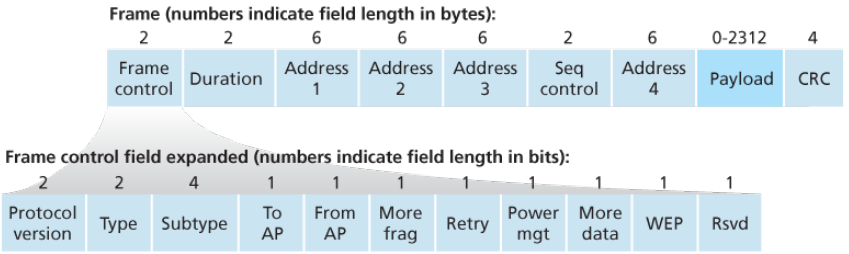
\includegraphics[width=\textwidth]{Frame80211.png}
\caption{Struttura di un frame 802.11}
\end{figure}
\subsubsection{Campi payload e CRC}
Tipicamente il payload consiste di un datagramma IP o di un pacchetto ARP, tipicamente limitato a 1500 bytes. Viene incluso un 32-bit cyclic redundancy check in modo da poter individuare errori. 
\subsubsection{Campi di indirizzo}
Il frame possiede quattro campi di indirizzo ognuno dei quali contiene un indirizzo MAC a 6 bytes. Tre campi sono necessari per scopi di internetworking: per muovere il datagframma dalla stazione all'AP al
router. Il quarto indirizzo \`e utilizzato quando un AP forward pacchetti in modalit\`a ad-hoc. 
\begin{itemize}
\item L'indirizzo 2 \`e l'indirizzo MAC della stazione che trasmette il frame. 
\item L'indirizzo 1 \`e l'indirizzo MAC della stazione wireless che deve ricevere il frame. 
\item L'indirizzo 3 contiene l'indirizzo MAC dell'interfaccia router della sottorete in cui si trova la stazione wireless, svolge un ruolo fondamentale di comunicazione tra la rete wireless e cablata.
\end{itemize}
\subsubsection{Sequence number, durata  e campi di frame control}
Il sequence number viene utilizzato per mappare l'acknowledgement al pacchetto su cui agisce. Il campo di durata include il periodo in cui una stazione riserva la connessione per inviare un frame e 
l'acknowledgement, incluso in RTS e CTS. Il campo frame control possiede molti sottocampi: il tipo e il sottotipo sono utilizzati per distinguere tra frame di associazione, di dati, RTS, CTS e ACK. I campi to e 
from definiscono i significati dei diversi campi di indirizzo. Il campo WEP indica se \`e utilizzata criptazione.
\subsection{Mobilit\`a nella stessa sottorete IP}
In modo da aumentare il raggio fisico di una LAN wireless vengono utilizzate multiple BSS con lo stessa sottorete IP. Si crea il problema di mantenere connesioni TCP spostandosi da una BSS all'altra. Quando
un dispositivo si sposta tra BSS mantiene l'indirizzo IP. Mentre il dispositivo si allontana individua un segnale che si indebolisce dall'Ap e comincia la scansione per un segnale pi\`u forte. Quando riceve un 
beacon frame si disassocia da quella corrente e si associa con l'altra mantenendo l'indirizzo IP e le connessioni TCP. Per aggiornare le tabelle di forwarding degli switch l'AP corrente invia un frame ethernet 
broadcast con l'indirizzo del dispositivo che si \`e appena connesso. 
\end{document}